\documentclass[a4paper,12pt,oneside]{book}%extreport
\usepackage{times} 
% \usepackage{multibib}
\usepackage{lipsum}
\usepackage{appendix}
\usepackage[shortlabels]{enumitem}
\usepackage{booktabs}
\usepackage{rotating} % Rotating table
\usepackage{hhline}
\usepackage{colortbl}
\usepackage{afterpage}
\usepackage{mathtools} %Fixes/improves amsmath
\usepackage{setspace}
\usepackage[utf8]{vietnam} 
\usepackage{amstext, amsmath,latexsym,amsbsy,amssymb, amssymb,amsthm,amsfonts,multicol, nccmath}
\usepackage[left=3cm,right=2cm,top=2.5cm,bottom=3cm,footskip=40pt]{geometry}
\usepackage{pdflscape}
\usepackage{apacite}
\usepackage{tikz}
\usepackage{array}
\newcolumntype{C}[1]{>{\centering\let\newline\\\arraybackslash\hspace{0pt}}m{#1}}
\usetikzlibrary{calc}
\usepackage{tabularx}
\usepackage{multicol}
\usepackage{array,color,colortbl}
\setcounter{secnumdepth}{4}

\usepackage{longtable}
\usepackage{diagbox}


\usepackage{tikz}
\usetikzlibrary{shapes.geometric, arrows.meta, positioning}


\tikzstyle{startstop} = [rectangle, rounded corners, minimum width=3cm, minimum height=1cm,text centered, draw=black, fill=red!30]
\tikzstyle{process} = [rectangle, minimum width=3cm, minimum height=1cm, text centered, draw=black, fill=blue!20]
\tikzstyle{decision} = [diamond, minimum width=2cm, minimum height=1cm, text centered, draw=black, fill=green!30]
\tikzstyle{arrow} = [thick,->,>=stealth]



 %\usepackage[square,numbers]{natbib}
\usepackage[square, comma, numbers, sort&compress]{natbib}
\setlength{\parindent}{1cm}
\usepackage{color}
\usepackage{indentfirst}
\usepackage{exscale,eucal}
\usepackage{fancyhdr}
\usepackage{fncychap}
\usepackage[chapter]{algorithm}
\usepackage{multirow}
\usepackage{graphicx}
\usepackage{algpseudocode}
\usepackage{tabularx,multicol,multirow,longtable}
\usepackage{etoolbox}
\usepackage{tikz}	\usetikzlibrary{calc,arrows,decorations.pathmorphing,backgrounds,positioning,fit,shapes,decorations.shapes, shapes.geometric, decorations.pathreplacing, decorations.text}
 
	\tikzstyle{block} = [draw,rectangle,thick,minimum height=2em,minimum width=2em,drop shadow,fill=blue!50]
	\tikzstyle{sum} = [draw,circle,inner sep=0mm,minimum size=2mm]
	\tikzstyle{connector} = [->,thick]
	\tikzstyle{line} = [very thick]
	\tikzstyle{branch} = [circle,inner sep=0pt,minimum size=1mm,fill=black,draw=black]
	\tikzstyle{axes} = [->,>=stealth',semithick]
	\tikzstyle{important line} = [very thick,draw=red]
	\tikzstyle{important text} = [rounded corners,fill=red!10,inner sep=1ex]
\usepackage{circuitikz}
\usepackage{pgfplots}
\pgfplotsset{compat=1.16}
\usepackage[numbers]{natbib}
\usepackage{titlesec}
\usepackage[labelsep=period]{caption}
\usepackage{subfigure}
\DeclareCaptionFormat{myformat}{\fontsize{13}{15}\selectfont#1#2#3}
\captionsetup{format=myformat}
\usepackage{titletoc}
\titlelabel{\thetitle.\,\,}
\titleformat{\chapter}[display] 
  {\fontsize{14}{16}\selectfont\bfseries\centering}
  {\MakeUppercase{\chaptertitlename}\ \thechapter}{0pt}{\fontsize{14}{16}\selectfont\MakeUppercase}
\titlespacing{\chapter}{0pt}{0pt}{40pt} 
\titleformat*{\section}{\fontsize{14}{14}\selectfont\bfseries}
\titleformat*{\subsection}{\fontsize{14}{14}\selectfont\bfseries\slshape}
\titleformat*{\subsubsection}{\fontsize{14}{14}\slshape}
\titleformat*{\paragraph}{\large\bfseries}
\titleformat*{\subparagraph}{\large\bfseries}
\graphicspath {{figures/}}

\titlespacing\section{0pt}{6pt plus 4pt minus 2pt}{1pt plus 2pt minus 2pt} 
\titlespacing\subsection{0pt}{6pt plus 4pt minus 2pt}{1pt plus 2pt minus 2pt}
\titlespacing\subsubsection{0pt}{6pt plus 4pt minus 2pt}{0pt plus 2pt minus 2pt}
\titlespacing\subsubsubsection{0pt}{6pt plus 4pt minus 2pt}{0pt plus 2pt minus 2pt}

\usepackage[subfigure]{tocloft} 

\cftsetpnumwidth{20pt}
\titlecontents{chapter}
  [0pt]
  {}
  {\fontsize{13.5}{14}\selectfont\MakeUppercase{\chaptername}\ \thecontentslabel.\,\,}
  {}
  {\cftdotfill{\cftdotsep}\contentspage} 
	\renewcommand{\cftsecaftersnum}{.}%
	\renewcommand{\cftsubsecaftersnum}{.}%

\usetikzlibrary{calc}
\newtheorem{definition}{\bf Định nghĩa}[chapter]
\newtheorem{theorem}{\bf Định lý}[chapter]
\newtheorem{lemma}{\bf Bổ đề}[chapter]

\renewcommand{\cftfigfont}{Hình~}
\renewcommand{\cfttabfont}{Bảng~ }
\floatname{algorithm}{Thuật toán}
\makeatletter
\renewcommand\@biblabel[1]{[#1]}
\renewcommand\harvardyearleft{\unskip~(}
\renewcommand\harvardyearright{\unskip )}
\makeatother
\renewcommand{\baselinestretch}{1.4}
\flushbottom
\renewcommand*{\bibfont}{\fontsize{13}{16}\selectfont}

\usepackage[hidelinks, unicode]{hyperref}

\begin{document}
\fontsize{13}{15.5}\selectfont

\pagestyle{empty}

\begin{titlepage}
    \centering
\begin{tikzpicture}[overlay,remember picture]
\centering
\draw[line width = 3pt] ($(current page.north west) + (1.215in,-0.7in)$) rectangle ($(current page.south east) + (-0.7in,0.7in)$);
\draw (0,-24.5) node[above]{\fontsize{12}{12}\selectfont{\textbf{HÀ NỘI - 2025}}};
\end{tikzpicture}
\vspace{-1cm}
\begin{center}
\MakeUppercase{\textbf{\fontsize{12}{12}\selectfont{Đại học quốc gia hà nội}}}

\noindent{\textbf {\MakeUppercase{\fontsize{12}{12}\selectfont {trường đại học công nghệ}}}}\\
%}
	\vspace{-0.5cm}
%\noindent\rule{10cm}{0.7pt}
\vspace{2cm}
\begin{figure} [!htb]
	\centering
	
\includegraphics[width=0.2\linewidth]{figures/UET_logo.jpg}
	\label{fig:uetlogo}
\end{figure}
\vspace{1.5cm}

		
	{\textbf {\fontsize{14}{14}\selectfont{Nguyễn Minh Hiếu}}}\\
\vspace{2cm}
\begin{center}
    \parbox{0.94\textwidth}{\centering
        {\fontsize{18}{18}\selectfont\textbf{\MakeUppercase{Nghiên cứu thiết kế lõi IP trích xuất đặc trưng sử dụng thuật toán MRELBP (Median Robust Extended Local Binary Pattern)}}}
    }
\end{center}
\vspace{3cm}
\MakeUppercase{\textbf{\fontsize{14}{14}\selectfont{{Khóa luận tốt nghiệp đại học hệ chính quy}}}}\\[3pt]
{\fontsize{14}{14}\textbf{\selectfont{Ngành: Kỹ thuật máy tính}}}
\end{center}


\end{titlepage}


\newpage
\pagestyle{plain}
\pagenumbering{gobble}
%\addcontentsline{toc}{chapter}{Trang phụ bìa}

\begin{center}
	\begin{tikzpicture}[overlay,remember picture]
\draw[line width = 3pt] ($(current page.north west) + (1.2in,-0.7in)$) rectangle ($(current page.south east) + (-0.7in,0.7in)$);
\draw (0,-24.2) node[above]{\fontsize{12}{12}\selectfont{\textbf{HÀ NỘI - 2025}}};
\end{tikzpicture}
\end{center}
\vspace{-1.5cm}
	\begin{center}
{\MakeUppercase{\textbf{\fontsize{12}{12}\selectfont{Đại học quốc gia hà nội}}}}

\noindent\textbf {\MakeUppercase{\fontsize{12}{12}\selectfont{trường đại học công nghệ}}}\\
	\vspace{-0.5cm}
%\noindent\rule{10cm}{0.7pt}
\vspace{4cm}
		

	{\textbf {\fontsize{14}{14}\selectfont{Nguyễn Minh Hiếu}}}\\
	\vspace{1.5cm}

\begin{center}
	\parbox{0.94\textwidth}{\centering
		{\fontsize{18}{18}\selectfont\textbf{\MakeUppercase{Nghiên cứu thiết kế lõi IP trích xuất đặc trưng sử dụng thuật toán MRELBP (Median Robust Extended Local Binary Pattern)}}}
	}
\end{center}
\vspace{3cm}
\MakeUppercase{\textbf{\fontsize{14}{14}\selectfont{{Khóa luận tốt nghiệp đại học hệ chính quy}}}}\\[3pt]
{\fontsize{14}{14}\textbf{\selectfont{Ngành: Kỹ thuật máy tính}}}

\end{center}
\vspace{1.5cm}
\begin{tabularx}{\linewidth}{>{\setlength\hsize{.0\hsize}}X>{\setlength\hsize{0.8\hsize}}X}
    & \fontsize{14}{14}\textbf{\selectfont{Cán bộ hướng dẫn: TS. Nguyễn Kiêm Hùng}} \newline
    \textit{(Ký tên)}
\end{tabularx}
             





\newpage
\def\baselinestretch{1.3}
\pagestyle{plain}
\pagenumbering{gobble}
\clearpage
\phantomsection

\addcontentsline{toc}{chapter}{Lời cam đoan}
\chapter*{Lời cam đoan}

Tôi xin cam đoan khóa luận tốt nghiệp \textbf{Nghiên cứu thiết kế lõi IP trích xuất đặc trưng sử dụng thuật toán Median Robust Extended Local Binary Pattern (MREBLBP)} là công trình nghiên cứu thực sự của tôi, được thực hiện dựa trên cơ sở lý thuyết, kiến thức chuyên ngành dưới sự hướng dẫn khoa học của TS. Nguyễn Kiêm Hùng.

Tôi xin cam đoan những công việc trong khóa luận thực hiện chưa từng được các tác giả khác đề xuất. Với sự hiểu biết của mình, tôi chắc chắn các số liệu, kết quả trong khóa luận là trung thực và chưa được công bố ở đâu và trong bất cứ công trình nào trừ công trình của tác giả và tài liệu tham khảo.

Nếu có gì sai trái, tôi xin hoàn toàn chịu trách nhiệm.

\vspace{1cm}
\hspace{7cm}\textit{Hà Nội, ngày ... tháng ... năm 2025}

\hspace{9.4cm}\textbf{Sinh viên}
\vspace{2.5cm}


\hspace{8.8cm}\textbf{Nguyễn Minh Hiếu}


\newpage
\clearpage
\phantomsection

\addcontentsline{toc}{chapter}{Lời cảm ơn}
\chapter*{Lời cảm ơn}

\textit{Đầu tiên, em xin cảm ơn đến khoa Điện Tử Viễn Thông, trường Đại học Công Nghệ Đại học Quốc Gia Hà Nội, các thầy cô đã tận tình chỉ dạy và trang bị cho em những kiến thức cần thiết trong suốt thời gian trên ghế giảng đường, làm nền tảng cho em có thể hoàn thành được bài đồ án này.}

\textit{Em xin gửi lời cảm ơn đến TS. Nguyễn Kiêm Hùng, thầy đã định hướng, hỗ trợ cho em từ trang thiết bị cho tới các kiến thức bổ ích, giải đáp các thắc mắc cũng như đề xuất những giải pháp phù hợp để công trình được hoàn thành. Thầy đã đồng hành cùng em một chặng đường rất dài trong suốt quãng thời gian qua. Em xin được gửi tới thầy những lời chúc tốt đẹp nhất.}

\vspace{1cm}
\hspace{7cm}\textit{Hà Nội, ngày ... tháng ... năm 2025}

\hspace{9.4cm}\textbf{Sinh viên}
\vspace{2.5cm}


\hspace{8.8cm}\textbf{Nguyễn Minh Hiếu}

 
\newpage
\clearpage
\phantomsection

\addcontentsline{toc}{chapter}{Tóm tắt}
\chapter*{\fontsize{13}{13}\selectfont{Tóm tắt}}
\fontsize{12}{12}\selectfont{
\noindent\textbf{Tóm tắt:}
Đồ án thực hiện thiết kế ở mức RTL một bộ trích xuất đặc trưng dựa trên thuật toán MRELBP (Median Robust Extended Local Binary Pattern). Phương pháp MRELBP được lựa chọn do khắc phục được hạn chế của LBP truyền thống trong việc nhận diện cấu trúc vĩ mô và tính nhạy với nhiễu. Việc thiết kế phần cứng chuyên biệt giúp tăng tốc xử lý trích xuất đặc trưng, đáp ứng với các yêu cầu cho hệ thống thời gian thực. Hệ thống SoC được triển khai trên nền tảng phần cứng ZCU106 Ultrascale và đánh giá độ chính xác bằng tập dữ liệu Outex-TC với ảnh kích thước 128x128. Kết quả thực thi cho thấy thời gian trích xuất đặc trưng nhanh gấp khoảng 1700 lần phiên bản xử lý bằng phần mềm với ngôn ngữ C++, độ chính xác với các tinh chỉnh với phiên bản phần cứng không thay đổi nhiều so với các phiên bản phần mềm. 

\vspace{0.5cm}
\noindent\textit{\textbf{Từ khóa:}} \textit{LBP, MRELBP, ZCU106, SoC.}
}
\newpage
\pagenumbering{roman}


\setlength{\parindent}{1cm}
\setlength{\parskip}{0.6ex}

\fontsize{13}{16}\selectfont
\renewcommand{\contentsname}{\vspace{-70pt}\centerline{\fontsize{14}{16}\selectfont\MakeUppercase{Mục lục}}}
\clearpage
\phantomsection
\addcontentsline{toc}{chapter}{Mục lục}
\tableofcontents
\clearpage
\clearpage
\phantomsection

\addcontentsline{toc}{chapter}{Tóm tắt}
\chapter*{\fontsize{13}{13}\selectfont{Tóm tắt}}
\fontsize{12}{12}\selectfont{
\noindent\textbf{Tóm tắt:}
Đồ án thực hiện thiết kế ở mức RTL một bộ trích xuất đặc trưng dựa trên thuật toán MRELBP (Median Robust Extended Local Binary Pattern). Phương pháp MRELBP được lựa chọn do khắc phục được hạn chế của LBP truyền thống trong việc nhận diện cấu trúc vĩ mô và tính nhạy với nhiễu. Việc thiết kế phần cứng chuyên biệt giúp tăng tốc xử lý trích xuất đặc trưng, đáp ứng với các yêu cầu cho hệ thống thời gian thực. Hệ thống SoC được triển khai trên nền tảng phần cứng ZCU106 Ultrascale và đánh giá độ chính xác bằng tập dữ liệu Outex-TC với ảnh kích thước 128x128. Kết quả thực thi cho thấy thời gian trích xuất đặc trưng nhanh gấp khoảng 1700 lần phiên bản xử lý bằng phần mềm với ngôn ngữ C++, độ chính xác với các tinh chỉnh với phiên bản phần cứng không thay đổi nhiều so với các phiên bản phần mềm. 

\vspace{0.5cm}
\noindent\textit{\textbf{Từ khóa:}} \textit{LBP, MRELBP, ZCU106, SoC.}
}
\newpage
\clearpage
\phantomsection
\addcontentsline{toc}{chapter}{Danh mục hình vẽ}
\renewcommand{\listfigurename}{\vspace{-70pt}\centerline{\fontsize{14}{16}\selectfont{\MakeUppercase{Danh mục   hình vẽ}}}}
\listoffigures
\fontsize{13}{16}\selectfont
\newpage
\clearpage
\phantomsection
\addcontentsline{toc}{chapter}{Danh mục bảng biểu}
\renewcommand{\listtablename}{\vspace{-70pt}\centerline{\fontsize{14}{16}\selectfont{\MakeUppercase{Danh mục bảng biểu}}}}
\listoftables
\fontsize{13}{16}\selectfont
\newpage

\pagenumbering{arabic}
\pagestyle{plain}

\clearpage
\phantomsection

\addcontentsline{toc}{chapter}{{Mở đầu}}
\chapter*{Mở đầu}
\noindent{\Large \textbf{Lý do chọn đề tài}}
\vspace{0.3cm}
\\ Với sự phát triển nhanh chóng của dữ liệu, phần cứng, các nhu cầu về ứng dụng của trí tuệ nhân tạo trong đời sống đang trở nên cấp thiết. Các phương pháp xử lý ảnh và thị giác máy hiện đại đã đóng một vai trò quan trọng trong các bài toán về phân loại hình ảnh, nhận diện mẫu, ... Kết cấu là khía cạnh cơ bản nhất của một bức tranh hay hình ảnh, góp phần tạo nên sự nhận dạng của bức tranh đó. Trong các bài toán về thị giác máy, thông tin kết cấu đóng vai trò quan trọng trong việc phân biệt các đối tượng có hình dạng tương tự nhưng thuộc các lớp khác nhau. Số lượng lớn các hình ảnh của vệ tinh, lâm nghiệp,... có thể được xác định  dựa vào kết cấu của chúng. Chẳng hạn, trong phân loại hình ảnh vệ tinh, kết cấu giúp phân biệt giữa rừng, đất nông nghiệp. 


Mặc dù các phương pháp học sâu đã ngày càng trở nên phổ biến hơn trong nhiều ứng dụng trong suốt thập kỷ qua, việc sử dụng các mô tả (descriptors) vẫn quan trọng trong nhiều lĩnh vực, những nơi mà không có đủ dữ liệu và tài nguyên tính toán để huấn luyện các mô hình phức tạp như CNN. MRELBP là một biến thể nâng cao của LBP (Local Binary Pattern), được thiết kế để khắc phục nhược điểm của LBP gốc như nhạy cảm với nhiễu và giới hạn trong việc phát hiện các cấu trúc có quy mô lớn. MRELBP sử dụng giá trị trung vị thay vì giá trị trung tâm để mã hóa thông tin kết cấu, giúp tăng tính ổn định khi gặp nhiễu và giữ lại thông tin tốt hơn ở các vùng có biến thiên nhỏ. Điểm mạnh của MRELBP nằm ở khả năng tính toán đơn giản. MRELBP có thể kết hợp với các mô hình huấn luyện cổ điển như SVM, KNN với tập dữ liệu không nhiều nhưng cho những kết quả tốt. Với CNN, đặc trưng được trích xuất thông qua các tầng tích chập và phi tuyến. Sau đó, đặc trưng được cung cấp vào những lớp huấn luyện phức tạp. Nhờ vào khả năng học biểu diễn mạnh mẽ, CNN vượt trội trong các bài toán phân loại hình ảnh phức tạp như nhận dạng khuôn mặt, nhận dạng đối tượng. Tuy nhiên, CNN cần một lượng lớn dữ liệu để huấn luyện, tài nguyên tính toán mạnh mẽ và tiêu tốn nhiều tài nguyên phần cứng vì cần rất nhiều các lớp tích chập để đưa ra được các đặc trưng nhiều ý nghĩa. Đã có những chứng minh cho thấy rằng việc sử dụng các phương pháp mô tả truyền thống như LBP đạt được những kết quả cao hơn CNNs trong nhiều tình huống \cite{Liu2017}. Do đó, LBP vẫn chứng minh được tính hiệu quả của mình. Tuy nhiên, LBP là một phương pháp nhạy cảm với các yếu tố về nhiễu và không có khả năng nắm bắt các cấu trúc vĩ mô. Có rất nhiều biến thể của LBP đã được đề xuất như Local Tenary Pattern (LTP), Extended Local Binary Pattern (ELBP),... Trong số đó, MRELBP là một trong những biến thể có được kết quả cao nhất với kết quả đạt lần lượt 99.82\%, 99.38\% và 99.77\% trong 3 tập dữ liệu của bộ dữ liệu Outex-TC \cite{Liu2016}.   


Việc ứng dụng các giải pháp trí tuệ nhân tạo vào đời sống là điều cần thiết, tuy nhiên, các thách thức về thời gian thực vẫn luôn là thách thức lớn. Các hệ thống nhúng nhỏ gọn dùng để thực hiện một chức năng chuyên biệt đang ngày càng chiếm vị trí quan trọng vì chúng có thể đạt được hiệu năng cao hơn rất nhiều. Do đó, mục tiêu của đồ án này là nghiên cứu và thực hiện phần cứng tăng tốc xử lý cho bộ trích xuất đặc trưng sử dụng MRELBP nhằm giảm thời gian tính toán. Để triển khai và kiểm thử trong thực tế, sinh viên sẽ xây dựng một hệ thống System on Chip (SoC) trên bo mạch ZCU106 với IP đã được thiết kế để đảm bảo tính chính xác, khả năng mở rộng và các yếu tố về tăng tốc thời gian.
\vspace{0.3cm}


\noindent{\Large \textbf{Phương pháp nghiên cứu}}
\vspace{0.3cm}

Trong khóa luận, để đạt được mục đích nghiên cứu, sinh viên đã tìm
hiểu các tài liệu, bài báo, tạp chí quốc tế,... có uy tín, thực hiện việc tính toán mô hình dữ liệu, phân tích số học để đưa ra các hướng giải quyết hợp lý, và sau đó kiểm nghiệm lại kết quả bằng hình thức mô phỏng bằng simulation trên phần mềm Vivado, triển khai tích hợp IP với hệ thống SoC và kiểm nghiệm lại với Integrated Logic Analyzer (ILA), so sánh kết quả đạt được với phần mềm đã có.  Cụ thể các phương pháp nghiên cứu sau đã được sử dụng trong khóa luận:
\renewcommand{\labelitemi}{$-$}
\begin{itemize}
	\item Sử dụng kỹ thuật Line Buffer để giảm truy cập bộ nhớ, đồng thời xây dựng nên các cửa sổ phù hợp cho việc tính toán.
	\item Sử dụng kiến trúc Systolic cho bộ tính toán trung vị.
	\item Nghiên cứu phương pháp cửa sổ dịch cho các bộ tính toán tổng ma trận.
	\item Tính toán, thiết kế bộ nội suy tuyến tính cho 24-bit dấu phẩy tĩnh.
	\item Mô phỏng và kiểm thử hệ thống trên phần mềm Vivado để đánh giá tính đúng đắn của thiết kế.
	\item Sử dụng công cụ ILA (Integrated Logic Analyzer) để phân tích tín hiệu nội bộ và xác thực hoạt động của hệ thống trên nền tảng FPGA.
	 
\end{itemize} 
\noindent{\Large \textbf{Nội dung nghiên cứu}}
\renewcommand{\labelitemi}{$-$}
\begin{itemize}
	\item Tìm hiểu về thuật toán MRELBP, đánh giá, so sánh với các biến thể khác của LBP và các thuật toán khác cho bài toán trích xuất đặc trưng.
	\item Xây dựng kiến trúc tổng thể và chi tiết cho toàn bộ hệ thống.
	\item Triển khai HDL, mô phỏng và kiểm thử.
	\item Tìm hiểu bo mạch ZCU106 và triển khai hệ thống SoC.
	\item Kiểm nghiệm lại toàn bộ hệ thống, so sánh và đánh giá kết quả đạt được.
\end{itemize} 
\noindent{\Large \textbf{Đóng góp của đề tài}}
\vspace{0.3cm}

Với sự hiểu biết của sinh viên, những kết quả nghiên cứu trong khóa luận đã đạt được mục đích nghiên cứu đề ra. Những kết quả này bao gồm:

\renewcommand{\labelitemi}{$-$}
\begin{itemize}
	\item Xây dựng được kiến trúc cho bộ tăng tốc phần cứng.
	\item Triển khai HDL, mô phỏng và kiểm tra.
	\item Kiểm nghiệm kết quả phần cứng và phần mềm với tập dữ liệu Outex-TC.
	\item Xây dựng hệ thống SoC sử dụng IP đã thiết kế.
	\item Đánh giá, phân tích kết quả thu được với kết quả mô phỏng và thực tế.
\end{itemize} 

\noindent{\Large \textbf{Bố cục của khóa luận}}
\vspace{0.5cm}

Nội dung chính của khóa luận được trình bày như sau:

\renewcommand{\labelitemi}{$-$}
\begin{itemize}
	\item \textbf{Mở đầu:} Trình bày mục đích, phương pháp nghiên cứu, nội dung, đóng góp và bố cục của khóa luận.
	\item \textbf{Chương 1: Cơ sở lý thuyết} - Các khái niệm cơ bản về các phương pháp trích xuất đặc trưng truyền thống, LBP, MRELBP, kỹ thuật xử lý, chuẩn giao tiếp và phần mềm sử dụng.
    \item  \textbf{Chương 2: Đặc tả kỹ thuật} - Đưa ra các mô tả và yêu cầu kỹ thuật cho từng mô-đun trong thiết kế IP.
	\item  \textbf{Chương 3: Thiết kế RTL} - Trình bày chi tiết ở mức RTL cho các mô-đun của thiết kế, thuật toán sử dụng.
    
	\item\textbf{Chương 4: Kiểm thử} - Trình bày phương pháp kiểm thử, mô phỏng và kiểm tra quá trình, kết quả hoạt động.
	\item  \textbf{Chương 5: Thực thi và đánh giá} - Thực hiện thực thi, đánh giá về bộ tăng tốc trên bo mạch ZCU106, các hạn chế và đề xuất phương hướng. 
    \item \textbf{Kết luận: }Tổng kết về công việc đã thực hiện và kết quả đạt được.
\end{itemize} 
\newpage
\clearpage
\phantomsection

\setcounter{chapter}{0}
\chapter[{CƠ SỞ LÝ THUYẾT}]{Cơ sở lý thuyết}
\section{Đặt vấn đề}
Sự phát triển mạnh mẽ của AI trong nhiều năm trở lại đây đã thúc đẩy mạnh mẽ tới sự phát triển của nhiều ngành nghề. Các ứng dụng và giải pháp AI xuất hiện ngày càng phổ biến trong nhiễu lĩnh vực bao gồm tài chính, chăm sóc sức khỏe, bảo mật, ... Năm 2022, thị trường AI toàn cầu được định giá khoảng 454,12 tỷ USD và dự kiến đạt 2.575,16 tỷ USD vào năm 2032 \cite{AIMARKET}. Theo khảo sát của McKinsey, tỷ lệ doanh nghiệp áp dụng AI ít nhất trong một chức năng đã tăng từ 20\% năm 2017 lên 50\% năm 2022 \cite{mckinsey}.

Với sự phát triển mạnh mẽ đó, các nhu cầu về việc tăng tốc AI bằng các phần cứng chuyên biệt cũng được tăng theo. Thị trường tăng tốc AI toàn cầu đạt khoảng 19.89 tỷ USD và dự kiến tăng trưởng với tốc độ CAGR 29.4\% từ 2024 đến 2030 \cite{aiaccelerator}. 
Field-Programmable Gate Arrays (FPGAs) là một trong những giải pháp linh hoạt, hiệu quả cho việc triển khai các thiết kế phần cứng tùy chỉnh cho từng ứng dụng AI. Với khả năng tính toán song song mạnh mẽ, ta có thể đạt được hiệu suất cao và đỗ trễ thấp kể cả đối với các thuật toán xử lý phức tạp. Bên cạnh đó, việc tối ưu hóa năng lượng tiêu thụ và tối ưu hóa I/O có thể đem lại những giá trị có lợi hơn cho nhiều giải pháp. Các nghiên cứu của Apriorit cũng chỉ ra rằng, FPGAs có thể cải thiện hiệu suất tổng thể của các ứng dụng AI \cite{apriorit}.
\section{Trích xuất đặc trưng}
\subsection{Khái niệm trích xuất đặc trưng}
Trích xuất đặc trưng là quá trình chuyển đổi các dữ liệu thô thành các dữ liệu số mà có thể xử lý bởi các mô hình mà vẫn đảm bảo được thông tin từ dữ liệu gốc. Việc trích xuất đặc trưng sẽ đem lại kết quả tốt hơn đối với nhiều thuật toán, giảm chiều và độ phức tạp của dữ liệu. Việc trích xuất đặc trưng có thể bao gồm việc lấy ra các dữ liệu đã có trong dữ liệu gốc hoặc tạo ra các đặc trưng mới bằng các kỹ thuật đặc trưng. Các đặc trưng này có thể coi là đặc tính của một đối tương dữ liệu. Từ những đặc tính đã được trích xuất, các mô hình có thể đạt được các kết quả tốt hơn trong khi lượng thông tin cần xử lý là ít hơn, đảm bảo được hiệu suất xử lý. 

Trong xử lý ảnh, trích xuất đặc trưng mô tả các thông tinh mang tính hình dạng có liên quan trong một mẫu để nhiệm vụ phân loại mẫu có thể thực hiện dễ dàng \cite{featureImgprocessing}. Có thể coi trích xuất đặc trưng là một dạng đặc biệt của giảm chiều dữ liệu. Mục tiêu chính của trích xuât đặc trưng là đạt được các thông tin liên quan của đối tượng từ dữ liệu gốc và biểu diễn chúng ở một chiều dữ liệu nhỏ hơn. Khi mà đầu vào của một thuật toán là quá lớn để xử lý, nó cần được loại bỏ dư thừa. Do đó, dữ liệu cần phải được giảm thiểu bằng cách biểu diễn dưới tập các đặc trưng có ý nghĩa. 
\subsection{Kết cấu thị giác}

\begin{figure} [h]
	\centering
	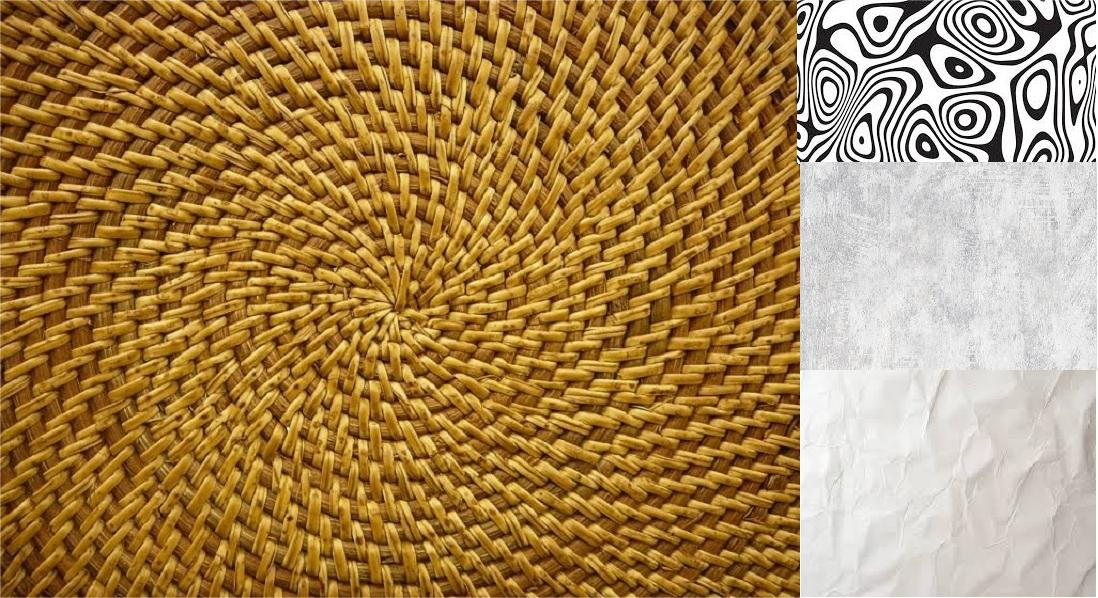
\includegraphics[width=0.8\linewidth]{figures/image1.png}
	\caption{Hình ảnh mẫu về kết cấu}
	\label{fig:image1}
\end{figure}
Texture hay kết cấu bề mặt là một khái niệm cơ bản trong lĩnh vực hình ảnh và thị giác máy tính đề cập đến các đặc điểm cơ bản của hầu hết mọi bề mặt tự nhiên có mặt ở khắp mọi nơi trong hình ảnh tự nhiên. Những đặc điểm này bao gồm kích thước, hình dáng, mật độ, sự sắp xếp và tỷ lệ của các thành phần cơ bản tạo nên thành phần đó. Trong thị giác máy tính, kết cấu đóng vai trò là một trong những đặc điểm quan trọng nhất để nhận diện và phân biệt các đối tượng hoặc các vùng quan tâm trong ảnh. Phân loại kết cấu là bài toán cơ bản được ứng dụng trong nhiều lĩnh vực như chuẩn đoán y khoa \cite{medicalImage}, dầu và gas \cite{textureBasedTechniques}, nông nghiệp \cite{smartFarming}, phân tích hình ảnh y sinh, hình ảnh vệ tinh, ... Mục tiêu chính của phân loại kết cấu là xây dựng một mô hình có khả năng mô tả nội dung kết cấu đã biết dựa trên dữ liệu huấn luyện. Tuy nhiên, để phân biệt được sự khác biệt giữa các kết cấu là vấn đề khá khó khăn vì các kết cấu thực tế thường có nhiều độ phân giải khác nhau, độ quay tùy ý và có thể được chiếu sáng bởi nhiều điện kiện chiếu sáng khác nhau. Điều này yêu cầu các phương pháp cần có khả năng phân tích được tính bất biến của đối tượng.


Một đặc trưng kết cấu tốt được mong đợi bởi đáp ứng 2 yếu tố: Độ phức tạp tính toán thấp cho phép phù hợp với các tác vụ phân loại thời gian thực và nắm bắt được thông tin kết cấu đại diện của một lớp kết cấu, sao cho các lớp kết cấu khác nhau có thể được phân biệt mặc dù có sự hiện diện của nhiều dạng hình ảnh khác nhau (bao gồm độ sáng, độ xoay, tỷ lệ, điểm nhìn, nhiễu, ...).


\subsection{Các phương pháp trích xuất đặc trưng}
Để phân loại kết cấu một cách hiệu quả, cần phải có các phương pháp mô tả và trích xuất đặc trưng của từng loại kết cấu. Có thể chia chúng thành 3 loại bao gồm: phương pháp thống kê, phương pháp mô hình và phương pháp bộ lọc \cite{analyticOfTexture}.

\begin{table}[h]
    \centering
    \renewcommand{\arraystretch}{1.3} % Tăng khoảng cách dòng
    \begin{tabular}{p{3cm} p{7cm} p{3cm} p{2cm}}
        \toprule
        \textbf{Phương pháp} & \textbf{Đặc điểm} & \textbf{Phân loại} & \textbf{Thuật toán} \\
        \midrule
        Thống kê & Phân tích sự phân bố không gian của các giá trị độ xám trong ảnh bằng cách tính toán các đặc trưng cục bộ, cung cấp các thông tin vể độ sáng, độ tương phản, ... & Bậc nhất, bậc 2 và bậc cao& GLCM, LBP, ... \\
        \midrule
        Mô hình & Xây dựng các mô hình toán học để mô tả kết cấu trong ảnh, sau đó trích xuất các tham số của mô hình này thông qua phân tích kết cấu. Bằng cách giả định rằng kết cấu được tạo ra bởi một quá trình ngẫu nhiên hoặc tuân theo một quá trình toán học cụ thể, các tham số của mô hình có thể được sử dụng làm đặc trưng để phân loại & Ngẫu nhiên, fractal, tự hồi quy & MRF, ... \\

                \midrule
        Bộ lọc & Sử dụng các bộ lọc để biến đổi ảnh gốc, sau đó năng lượng của các phản hồi bộ lọc được tính toán tạo thành các đặc trưng kết cấu & Miền không gian, miền tần số, miền không gian - tần số & Gabor filters, Wavelet transforms, ... \\
                        \bottomrule

    \end{tabular}
    \caption{Các phương pháp trích xuất đặc trưng}
    \label{tab:texture_analysis}
\end{table}

\newpage
\subsection{Local Binary Pattern}
\label{sec:lbp}
Một vài cách tiếp cận về tính bất biến của độ quay của kết cấu có thể kể đến ảnh cực đồ \cite{polarograms}. Một vài cách khác được đề xuất bằng cách chính sửa các phương pháp đã có như mô hình MRF (Markov Random Field), bộ lọc Gabor hoặc LBP. Trong đó, LBP là một trong những phương pháp thường được sử dụng để mô tả các mô tả kế cấu bởi độ phức tạp tính toán thấp, dễ triển khai và bất biến với sự thay đổi ánh sáng đơn điệu \cite{Liu2016}.

Local Binary Pattern (LBP) là một phương pháp thuộc nhóm phương pháp thống kê, được sử dụng để mô tả các mô tả kết cấu (texture descriptors). LBP được giới thiệu lần đầu tiên vào năm 1994 \cite{firstLBP}, có khả năng mô tả các cấu trúc không gian của một vùng bên trong hình ảnh bằng cách mã hóa sự khác biệt giữa giá trị điểm ảnh ở vị trí trung tâm vùng với các điểm ảnh xung quanh nó, giá trị thập phân của mẫu nhị phân sau khi so sánh được sử dụng làm nhãn cho giá trị điểm ảnh ở trung tâm đó. Hình \ref{fig:lbp_oper} mô tả hoạt động của LBP với điểm ảnh trung tâm là  $x_c$, kết quả được tính toán bằng cách so sánh giá trị với p các giá trị hàng xóm $\{x_{r, p, n}\}_{n=0}^{p-1}$ được phân bố đồng đều trên một đường tròn bán kính r, kết quả được tính theo công thức sau:
\begin{equation}
	LBP_{r, p}(x_c) = \sum_{n=0}^{p-1}s(x_{r,p, n} -x_c)2^n 
\begin{cases} 
1, & x \geq 0 \\ 
0, & x < 0 
\end{cases}
\end{equation}


\begin{figure} [h]
	\centering
	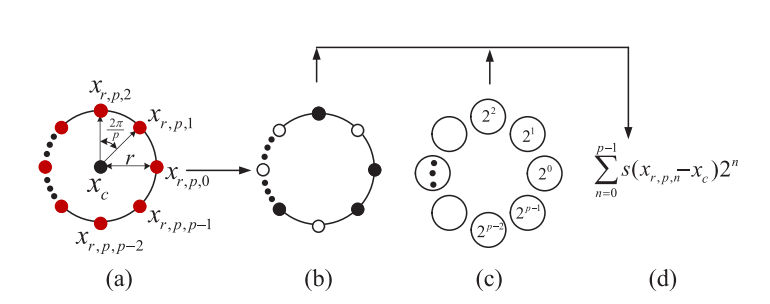
\includegraphics[width= 1\linewidth]{figures/lbp_oper.png}
	\caption{Hoạt động của LBP với bán kính r và p điểm ảnh xung quanh \cite{Liu2016}}
	\label{fig:lbp_oper}
\end{figure} 

Với $s()$ là hàm dấu (sign function). Nếu tọa độ của $x_c$ là (0, 0) thì tọa độ của các điểm xung quanh $x_{p, r, n}$ là $(-rsin(2\pi n/p), rcos(2\pi n /p))$. Giá trị của $x_{p,r,n}$ có thể không là giá trị ở vị trí trung tâm mà có thể sẽ được ước tính bằng phương pháp nội suy.
\begin{figure} [h]
	\centering
	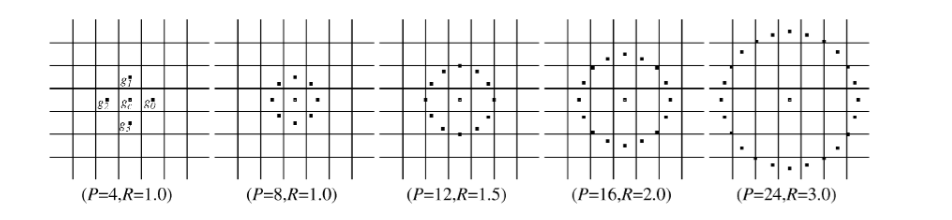
\includegraphics[width= 1\linewidth]{figures/lbpCircularSymmetric.png}
	\caption{LBP với các mẫu bán kính và điểm ảnh lân cận\cite{Ojala}}
	\label{fig:lbpCircularSymmetric}
\end{figure} 
Tuy nhiên, LBP vẫn bị ảnh hưởng nhiều bởi yếu tố độ xoay. Để giảm thiểu sự ảnh hưởng này, một biến thể LBP khác được đưa ra để đạt được sự bất biến của độ quay. Với p giá trị điểm ảnh lân cận, dựa vào toán tử LBP có thể có $2^p$ giá trị đầu ra khác nhau. Khi ảnh được xoay, giá trị nhị phân có được ở vị trí thứ x sẽ di chuyển xung quanh giá trị trung tâm. Do đó, để giảm sự ảnh hưởng của sự quay, Ojala \cite{Ojala} đã định nghĩa ra một định nghĩa như sau:

\begin{equation}
	LBP_{r, p}^{ri} = min\{ROR(LBP_{r, p}i) |  i = 0, 1, 2, ..., P-1\}
\end{equation}

Với $ROR(x, i)$ thực hiện việc dịch bit sang phải theo hình tròn. Với p điểm ảnh xung quanh, thì ta sẽ cần dịch đi i lần. Có thể hiểu đơn giản là ta sẽ đi tìm giá trị nhỏ nhất của một dãy bit bằng cách dịch chúng. Ví dụ với 8 điểm ảnh xung quanh, với dãy bit là $10000000_2$, ta có thể có rất nhiều giá trị như $01000000_2$ ứng với $64_{10}$ hay $00000001_2$ ứng với $1_{10}$. Nhưng khi thực hiện toàn bộ phép dịch và lấy giá trị nhỏ nhất, ta có thể đạt được giá trị là $1_{10}$, và đây là giá trị duy nhất. Các điểm ảnh khác nếu có thể đạt được giá trị như $00010000_2$, sau đó cũng được chuyển thành giá trị $1_{10}$ ở hệ thập phân. Hình \ref{fig:lbpRotation} mô tả số giá trị đặc trưng có thể có với p = 8. Mẫu số 0 giúp nhận biết điểm sáng, số 8 giúp nhận biết điểm tối, mẫu số 4 giúp nhận biết biên.  


\begin{figure} [h]
	\centering
	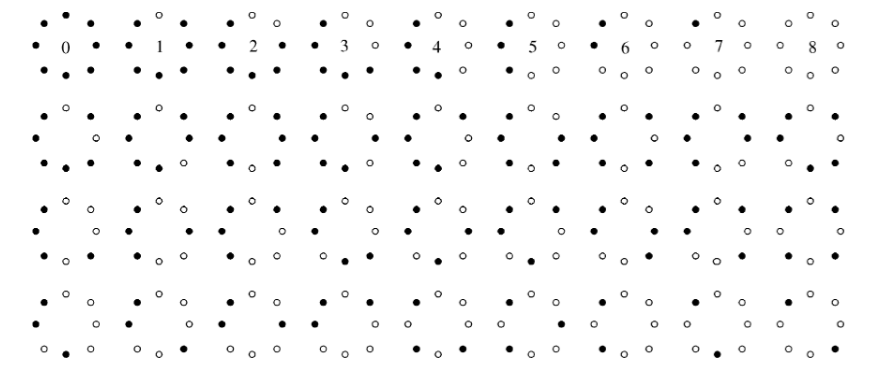
\includegraphics[width= 1\linewidth]{figures/lbpRotation.png}
	\caption{36 giá trị đặc trưng ứng với 8 giá trị điểm ảnh lân cận \cite{Ojala}}
	\label{fig:lbpRotation}
\end{figure} 

Để cải thiện thêm về tính bất biến của độ xoay, một khái niệm được đưa ra là \textbf{đồng nhất (uniform)}. Một mẫu đồng nhất sẽ chứa ít sự thay đổi về mặt không gian. Chúng hoạt động như các khuôn mẫu cho các cấu trúc vi mô như điểm sáng (0), vùng tối (8) hoặc các cạnh có độ cong âm hay dương (1-7). Để định nghĩa một mẫu là đồng nhất, Ojala giới thiệu một phương pháp gọi là U("pattern"), chúng chỉ đo lường sụ thay đổi về mặt không gian (tức là sự thay đổi các bit từ 0 thành 1 hay từ 1 thành 0). Ví dụ, mẫu $00000000_2$ và mẫu $11111111_2$ có giá trị U bằng 0, trong khi đó 7 giá trị khác ở dòng đầu ở hình \ref{fig:lbpRotation}
 có giá trị U bằng 2 vì có chính xác 2 lần thay đổi bit từ 0 thành 1 và từ 1 thành 0. Trong khi đó, 27 mẫu còn lại có giá tị U ít nhất là 4. Từ đó, ta có định nghĩa về LBP đồng nhất như sau (đặt ngưỡng giá trị của U tối đa là T):

 \begin{equation}
     LBP_{r, p}^{riuT} = 
     \begin{cases}
         \sum_{i=0}^{p-1}s(gi - gc)  & \text{nếu} \space U(LBP) \leq T
         \\
         p+1 & \text{còn lại}
     \end{cases}
     \label{eq:riu2}
 \end{equation}
 Với
 \begin{equation}
     U(LBP_{r, p}) = | s(g_{p-1} - g_c) - s(g_0 -g_c)| + \sum_{i = 1}^{p-1}|s(g_i - g_c) - s(g_{i-1} - g_c)| 
 \end{equation}
 
\begin{figure} [h]
	\centering
	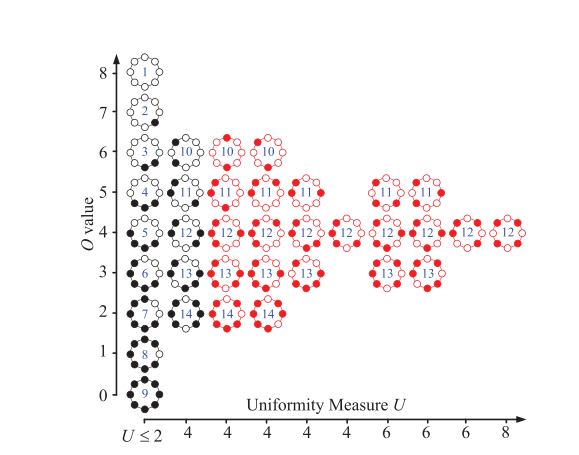
\includegraphics[width= 0.8\linewidth]{figures/lbpU.png}
	\caption{Số lượng các mẫu theo U với p = 8 \cite{Liu2016}}
	\label{fig:lbpU}
\end{figure} 

 Từ \textbf{riuT} thể hiện việc sử dụng mẫu đồng nhất với ngưỡng T và áp dụng việc dịch phải theo hình tròn. Nếu chỉ áp dụng mẫu đồng nhất T, ta có thể sử dụng từ \textbf{uT}. Ví dụ với T = 2, thì ta sẽ có phiên bản $LBP_{r, p}^{u2}$. Với p = 8, ta sẽ có tập hợp các mẫu ứng với giá trị của U, được mô tả trong hình \ref{fig:lbpU}.
\subsection{Các biến thể của LBP}
Có rất nhiều các biến thể của LBP đã được nghiên cứu nhằm mục đích tăng cường sự mạnh mẽ và khả năng phân biệt. Từ khảo sát từ Di Huang, Caifeng Shan, Mohsen Ardabilian, Yunhong Wang, Liming Chen \cite{lbpVariantSurvey}, bảng \ref{tab:lbpVariant} mô tả một vài biến thể của LBP. 


\begin{table}[h]
    \centering
    \renewcommand{\arraystretch}{1.3} % Tăng khoảng cách dòng
    \begin{tabular}{p{4cm} p{7cm} p{3cm}}
        \toprule
        \textbf{Tên biến thể} & \textbf{Đặc điểm} & \textbf{Mục tiêu} \\
        \midrule
        Extended LBP & Sử dụng thêm một số đơn vị nhị phân bổ sung  & Nâng cao khả năng phân biệt
        \\ \midrule
        Completed LBP & Xem xét cả dấu và độ lớn của các mẫu cục bộ & Nâng cao khả năng phân biệt
        \\ \midrule
        Soft LBP & Kết hợp các thành viên trong việc biểu diễn các mẫu cục bộ & Tăng cường khả năng chống nhiễu
        \\ \midrule 
        Local Tenary Binary & Sử dụng ngưỡng để tạo sự khác biệt & Tăng cường khả năng chống nhiễu
        \\
                        \bottomrule

    \end{tabular}
    \caption{Một vài biến thể của LBP}
    \label{tab:lbpVariant}
\end{table}



\newpage
\subsection{Median Robust Extended Local Binary Pattern}

\begin{figure} [h]
	\centering
	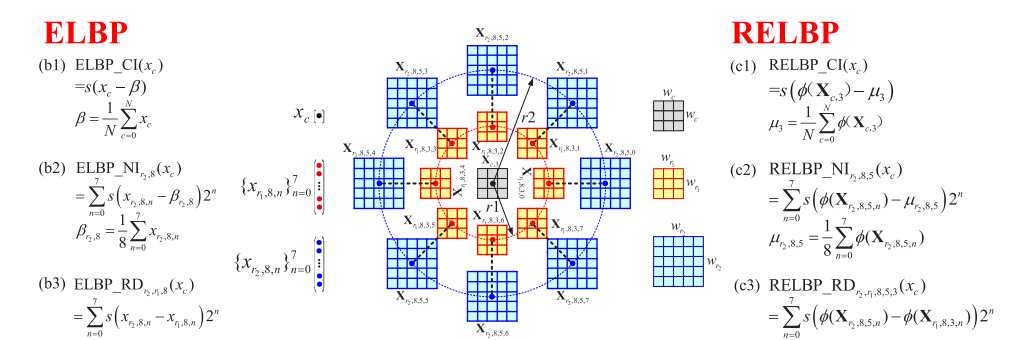
\includegraphics[width= 1\linewidth]{figures/elbpARelbp.png}
	\caption{Sự khác nhau giữa trích xuất đặc trưng của ELBP và RELBP \cite{Liu2016}}
	\label{fig:elbpARelbp}
\end{figure} 
Với ELBP, một trong những khuyết điểm của nó là bị ảnh hưởng nhiều bởi nhiễu, do đó cần phải thay thế cường độ pixel riêng lẻ tại một điểm bằng một số biểu diễn trên một vùng. Các phương pháp đáng chú ý theo hướng này bao gồm BRIEF, BRISK và FREAK, trong đó trong mọi trường hợp, một vector mô tả nhị phân được đạt được bằng cách so sánh cường độ của một số cặp pixel sau khi áp dụng làm mịn Gaussian để làm giảm độ nhiễu. Li Liu \cite{Liu2016} xem xét tác động của việc thay thế các giá trị độ xám riêng lẻ tại các điểm lấy mẫu bằng cách dùng các bộ lọc đơn giản từ ảnh gốc và các vùng trong ảnh gốc. Đặc trưng của ELBP được thay đổi từ cường độ pixel tại các điểm riêng lẻ được thay thế bằng phản hồi từ các bộ lọc $\phi()$. Hình \ref{fig:elbpARelbp} thể hiện sự khác nhau giữa 2 phiên bản. Từ đó, định nghĩa ra Robust Extended Local Binary Pattern (RELBP) với các mô tả như sau:

\begin{enumerate}
    \item Biểu diễn điểm ảnh trung tâm 
    \begin{equation}
        RELBP\_CI(x_c) = s(\phi(\mathbf{X}_{c, w}) - \mu_w)
         \label{eq:relbp_ci}
    \end{equation}
    $\begin{cases}
    \phi(\mathbf{X}_{c,w}) \text{ là kết quả sau khi áp dụng bộ lọc lên điểm ảnh } X, \\
    \text{Vùng cục bộ có kích thước } w \times w \text{ ở xung quanh vị trí điểm ảnh trung tâm}, \\
    \mu_w \text{ kí hiệu cho giá trị trung bình của } \phi(X_{c,w}) \text{ trong toàn bộ bức ảnh}.
\end{cases}$



    \item Biểu diễn các giá trị lân cận
\begin{equation}
    \begin{aligned}
        RELBP\_NI_{r, p}(x_c) &= \sum_{n=0}^{p-1}s(\phi(\mathbf{X}_{r, p, w_r, n}) - \mu_{r, p, w_r}) 2^n \\
        \mu_{r, p, w_r} &= \frac{1}{p}\sum_{n =0}^{p-1}\phi(\mathbf{X}_{r, p, w_r, n})
    \end{aligned}
             \label{eq:relbp_ni}
\end{equation}

    \item Biểu diễn chênh lệch hướng tâm
    \begin{equation}
        RELBP\_RD_{r, r-1, p, w_r, w_{r-1}}(x_c) = \sum_{n=0}^{p-1}s(\phi(\mathbf{X}_{r, p, w_r, n}) - \phi(\mathbf{X}_{r-1, p, w_{r-1}, n}))2^n
             \label{eq:relbp_rd}
\end{equation}
\end{enumerate}

Các công thức \ref{eq:relbp_ci}, \ref{eq:relbp_ni}, \ref{eq:relbp_rd} là cách thực hiện tính toán đặc trưng với các thông tin có trong ảnh. Median Robust Extended Local Binary Pattern là phiên bản RELBP với bộ lọc được sử dụng là median. Phương pháp này có ưu điểm so với LBP truyền thống là mạnh hơn trước nhiễu và sự thay đổi của ảnh sáng. Nó nắm bắt thông tin kết cấu và thông tin không gian tốt hơn thông qua bộ lọc trung vị và mở rộng mẫu bên trong ảnh. Tuy vậy, MRELBP vẫn tồn tại một số nhược điểm như bị giới hạn ở các mẫu cục bộ. Tuy đã được mở rộng nhưng các kỹ thuật LBP vẫn tập trung vào các chi tiết cục bộ mà có thể bỏ sót các thay đổi ở kết cấu quy mô lớn. Kích thước bán kính cố định cũng là một nhược điểm, làm nó thiếu đi tính linh hoạt ở nhiều tỷ lệ khác nhau.

\section{Nền tảng về thiết kế số}
\subsection{Tổng quan về thiết kế số}
% thiet ke so la gi, dac trung, rtl, 
Thiết kế số là quá trình thiết kế và tạo ra các sản phẩm bằng máy tính, sử dụng dữ liệu số để tạo ra các sản phẩm. Nó liên quan đến việc thiết kế các mạch và hệ thống số thường được thực hiện ở cấp độ trừu tượng Register-Transfer Level (RTL). RTL mô tả chức năng của mạch thông qua sự chuyển đổi dữ liệu giữa các thanh ghi. Mã RTL thường được viết bằng các ngôn ngữ như Verilog, VHDL, ...

\textbf{Mạch logic tổ hợp} là mạch mà trạng thái đầu ra của mạch chỉ phụ thuộc và tổ hợp các trạng thái đầu vào ở cùng thời điểm mà không phụ thuộc vào thời điểm trước đó.

\textbf{ Mạch logic tuần tự} là mạch có tính chất nhớ, có trễ. Trạng thái tiếp theo của mạch phụ thuộc vào giá trị kích thích ở lối vào và trạng thái hiện tại của mạch. Mạch tuần tự thường hoạt động theo sự điều khiển của tín hiệu clock. Có 2 loại mạch logic tuần tự là mạch đồng bộ và không đồng bộ. Mạch đồng bộ là mạch là sẽ thay đổi giá trị theo 1 giá trị tham chiếu đến (thường là clock). Còn mạch không đồng bộ là mạch mà sẽ thay đổi giá trị ngay khi tín hiệu điều khiển hoạt động đó thay đổi giá trị. 

\subsection{Máy trạng thái hữu hạn}
Máy trạng thái hữu hạn, viết tắt là FSM, là một thành một phần được sử dụng phổ biến trong thiết kế số với ưu điểm là dễ dàng kiểm soát quá trình hoạt động của mạch. 
\begin{figure}[!ht]
    \centering
    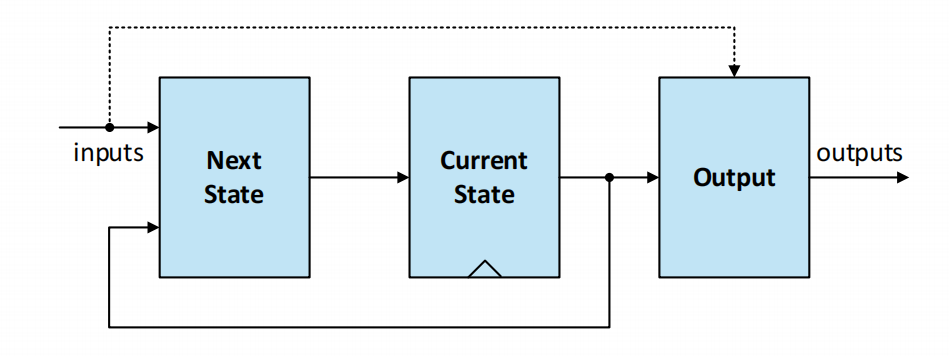
\includegraphics[width=1\linewidth]{figures/fsm.png}
    \caption{Máy trạng thái hữu hạn}
    \label{fig:fsm}
\end{figure}
Về cơ bản, máy trạng thái hữu hạn sẽ có 3 thành phần cơ bản như mô tả tại hình \ref{fig:fsm}. 
\begin{itemize}
    \item Mạch tạo trạng thái kế tiếp (Next State logic): Là mạch tổ hợp phụ thuộc vào đầu vào FSM và giá trị trạng thái hiện tại lấy từ bộ nhớ trạng thái
    \item Bộ nhớ trạng thái hay trạng thái hiện tại: Là phần tử lưu trữ trạng thái của FSM, nó có thể là Flip-Flop, Latch, ... Lấy đầu vào từ mạch tạo trạng thái kế tiếp. 
    \item Mạch tạo đầu ra: Là mạch tổ hợp tạo ra giá trị đầu ra tương ứng với trạng thái hiện tại của FSM. Mạch này lấy đầu vào là giá trị trạng thái hiện tại và có thể tổ hợp thêm đầu vào FSM. 
\end{itemize}


FSM được chia làm 2 loại là máy Moore và Mealy. Máy Moore là máy mà có mạch tạo đầu ra chỉ phụ thuộc vào trạng thái hiện tại của FSM. Hình \ref{fig:fsm} trên nếu bỏ đường gạch nét đứt vào khối tạo đầu ra thì là máy Moore. Máy Mealy là máy mà có mạch tạo đầu ra phụ thuộc vào cả trạng thái hiện tại và giá trị đầu vào. Hình \ref{fig:fsm} với đường nét đứt nối vào mạch tạo đầu ra mô tả một máy Mealy.
\subsection{Pipelining}
Kỹ thuật đường ống (Pipelining) là một kỹ thuật được sử dụng trong các mạch số đồng bộ để tăng tần số hoạt động tối đa. Kỹ thuật này liên quan đến việc chèn thêm các thanh ghi ở các đường dẫn quan trọng, làm giảm số lượng logic giữa mỗi thanh ghi. Ít logic hơn sẽ tiêu tốn ít thời gian để thực hiện hơn, từ đó gia tăng tần số hoạt động tối đa.

Đường dẫn quan trọng (critical path) trong mạch là đường dẫn giữa 2 thanh ghi liên tiếp với đỗ trễ cao nhất. Điều đó cũng tương đương với việc thời gian để có giá trị đầu ra giữa 2 thanh ghi này là lâu nhất.  Hình \ref{fig:pipeline1} mô tả mạch trước khi được pipelining. Trong đó, thời gian thực hiện 2 mạch tổ hợp giữa 2 thanh ghi là thời gian của mạch A cộng với mạch B. Do đó, thời gian tính toán tổ hợp tốn 20ms. Ở hình \ref{fig:pipeline2} đã thực hiện pipelining bằng cách chèn vào giữa A và B một thanh ghi, do đó thời gian tối đa trong tính toán tổ hợp chỉ là 15ms. Do đó, kĩ thuật pipelining sẽ giúp tăng lên tần số hoạt động tối đa của mạch. 
\begin{figure}[!ht]
    \centering
    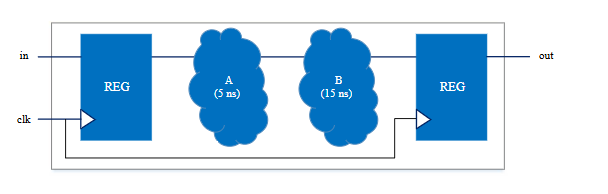
\includegraphics[width=\linewidth]{figures/pipeline1.png}
    \caption{Mạch trước khi pipelining}
    \label{fig:pipeline1}
\end{figure}
\begin{figure}[!ht]
    \centering
    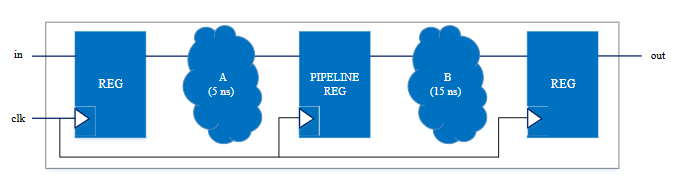
\includegraphics[width=\linewidth]{figures/pipeline2.png}
    \caption{Mạch sau khi pipelining}
    \label{fig:pipeline2}
\end{figure}
\subsection{Giao diện AXI4-Stream}
Trong một hệ thống System on Chip (SoC), BUS là thành phần chính kết nối các master và slave. Nó giúp các master có thể truy xuất (đọc/ghi) các slave bằng cách chuyển thông tin điều khiển từ master đến slave, đồng thời chuyển dữ liệu và thông tin phản hồi từ slave đến master. AXI (Advanced eXtensible Interface) là một trong các giao thức BUS trong họ AMBA (Advanced Microcontroller Bus Architecture), được phát triển bởi hãng ARM. 

AXI4-Stream là một liên kết điểm tới điểm, bên gửi là master còn bên nhận là slave. Để giao tiếp được giữa hai bên, cần một quá trình gọi là bắt tay. Hình \ref{fig:axi4} mô tả quá trình truyền dữ liệu đối với kênh AXI4-Stream. Tín hiệu \textbf{tvalid} được phát bởi bên truyền và \textbf{tready} được phát bởi bên nhận. Tín hiệu \textbf{tvalid} chỉ ra rằng dữ liệu \textbf{tdata} là hợp lệ. Tín hiệu \textbf{tready} chỉ ra rằng bên nhận sẵn sàng để nhận dữ liệu. Khi mà cả \textbf{tvalid} và \textbf{tready} đều ở mức cao thì quá trình truyền diễn ra.


\begin{figure}[!ht]
    \centering
    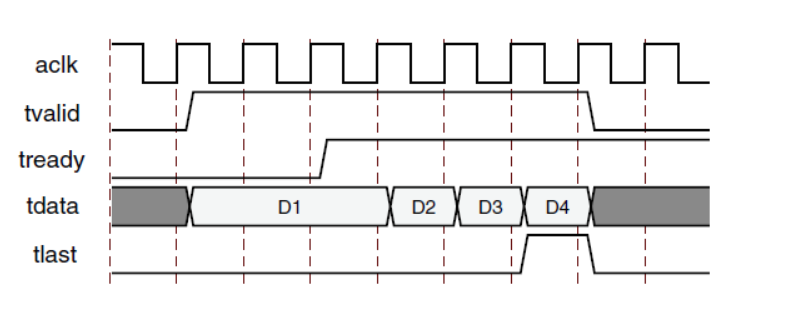
\includegraphics[width=\linewidth]{figures/axi4.png}
    \caption{Truyền dữ liệu ở kênh AXI4-Stream}
    \label{fig:axi4}
\end{figure}
\section{Phần mềm thiết kế và mô phỏng Vivado}
\section{Luồng thiết kế}
\newpage
\clearpage
\phantomsection

\setcounter{chapter}{1}
\chapter[{ĐẶC TẢ KỸ THUẬT}]{Đặc tả kỹ thuật}

%\section{Đặc tả kỹ thuật}
Chương này sẽ cung cấp các thông tin về các yêu cầu chức năng và phi chức năng của IP cần thiết kế, từ mô-đun lớn nhất đến các mô-đun nhỏ hơn. Các thông tin về đặc tả kỹ thuật sẽ bao gồm thông tin về chức năng, danh sách tham số và tín hiệu của mô-đun, kiến trúc ở mức hành vi và mô tả dạng sóng của mô-đun.

\section{Yêu cầu hệ thống }
Bảng \ref{tab:non_functional} đây mô tả các yêu cầu hệ thống cho IP (bao gồm yêu cầu chức năng và yêu cầu phi chức năng):
\begin{table}[!ht]
    \centering
    \renewcommand{\arraystretch}{1.3} % Tăng khoảng cách dòng
        \caption{Các yêu cầu phi chức năng cho thiết kế}
    \begin{tabular}{p{5cm} p{10cm} }
        \toprule
        \textbf{Yêu cầu} & \textbf{Mô tả} \\
        \midrule
        Chức năng & Thực hiện trích xuất đặc trưng sử dụng thuật toán MRELBP
        \\ \midrule
        Thông số kỹ thuật & 
        \begin{tabular}[t]{@{}l@{}}
Các thông số thuật toán: r = 2, 4, 6; p = 8 \\
Độ rộng dữ liệu: Đầu vào 8-bit, đầu ra 32-bit \\
Kích thước ảnh đầu vào: có thể tùy chỉnh theo tham số cấu hình \\
Số lượng dữ liệu đầu ra: 600 dữ liệu \\
Độ chính xác: dấu phẩy tĩnh (16-bit thập phân, 8-bit phần nguyên)
\end{tabular} 
\\
        
        \midrule
        Hiệu suất (Performance) & Tần số hoạt động tối thiểu 100 MHz
        \\ \midrule
        Tính đồng bộ & Tất cả các tín hiệu đồng bộ theo 1 clock chính
        \\ \midrule
        Reset & Tất cả các mô-đun tuân theo reset đồng bộ
        \\ \midrule
        Tài nguyên sử dụng & Tối đa 30000 LUTs, 30000 Registers, 200 DSPs, 100 BRAM 
        \\ \midrule
        Khả năng kiểm thử & Hỗ trợ kiểm thử test-bench ngẫu nhiên và test-bench trực tiếp
        \\ \midrule
        Chuẩn giap tiếp & Có thể tương thích với chuẩn AXI4-Stream
        \\ \midrule
        Tương thích công cụ & Có thể tổng hợp trên các phần mềm như Vivado, Quartus, ...
        \\ \midrule
        Khả năng tích hợp & Có thể giao tiếp IP đối với các IP khác như DMA, ...
        \\ \midrule
        Độ bao phủ & Tối thiểu 80\% về mặt chức năng
        \\ \midrule
        Kiểm thử tự động & Xây dựng hệ thống giúp kiểm thử về mặt chức năng một cách tự động
        \\
        
                        \bottomrule

    \end{tabular}

    \label{tab:non_functional}
\end{table}
\section{Xác định thiết kế}
\subsection{Tối ưu thuật toán phù hợp với phần cứng}
Đồ án sẽ xây dựng IP trích xuất đặc trưng sử dụng thuật toán Median Robust Extended Local Bianry Pattern. Đây là một thuật toán hoạt động tương đối phức tạp với 3 loại đặc trưng được tính toán theo các công thức \ref{eq:relbp_ci}, \ref{eq:relbp_ni}, \ref{eq:relbp_rd}. Tuy nhiên, đối với công thức \ref{eq:relbp_ci}, việc phải lưu lại toàn bộ bức ảnh để tính trung bình sẽ gây ảnh hưởng lớn về mặt thời gian và lưu trữ, do đó, để cải tiến, ta sẽ có mô tả như sau:
    \begin{equation}
        RELBP\_CI(x_c) = s(\phi(\mathbf{X}_{c, w}) - \mu_w)
         \label{eq:relbp_ci_op}
    \end{equation}
    $\begin{cases}
    \phi(\mathbf{X}_{c,w}) \text{ là kết quả sau khi áp dụng bộ lọc lên điểm ảnh } X, \\
    \text{Vùng cục bộ có kích thước } w \times w \text{ ở xung quanh vị trí điểm ảnh trung tâm}, \\
    \mu_w \text{ kí hiệu cho giá trị trung bình của } \phi(X_{c,w}) \text{ trong một vùng cục bộ kích thước w x w}.
\end{cases}$

\begin{figure} [!hht]
	\centering
	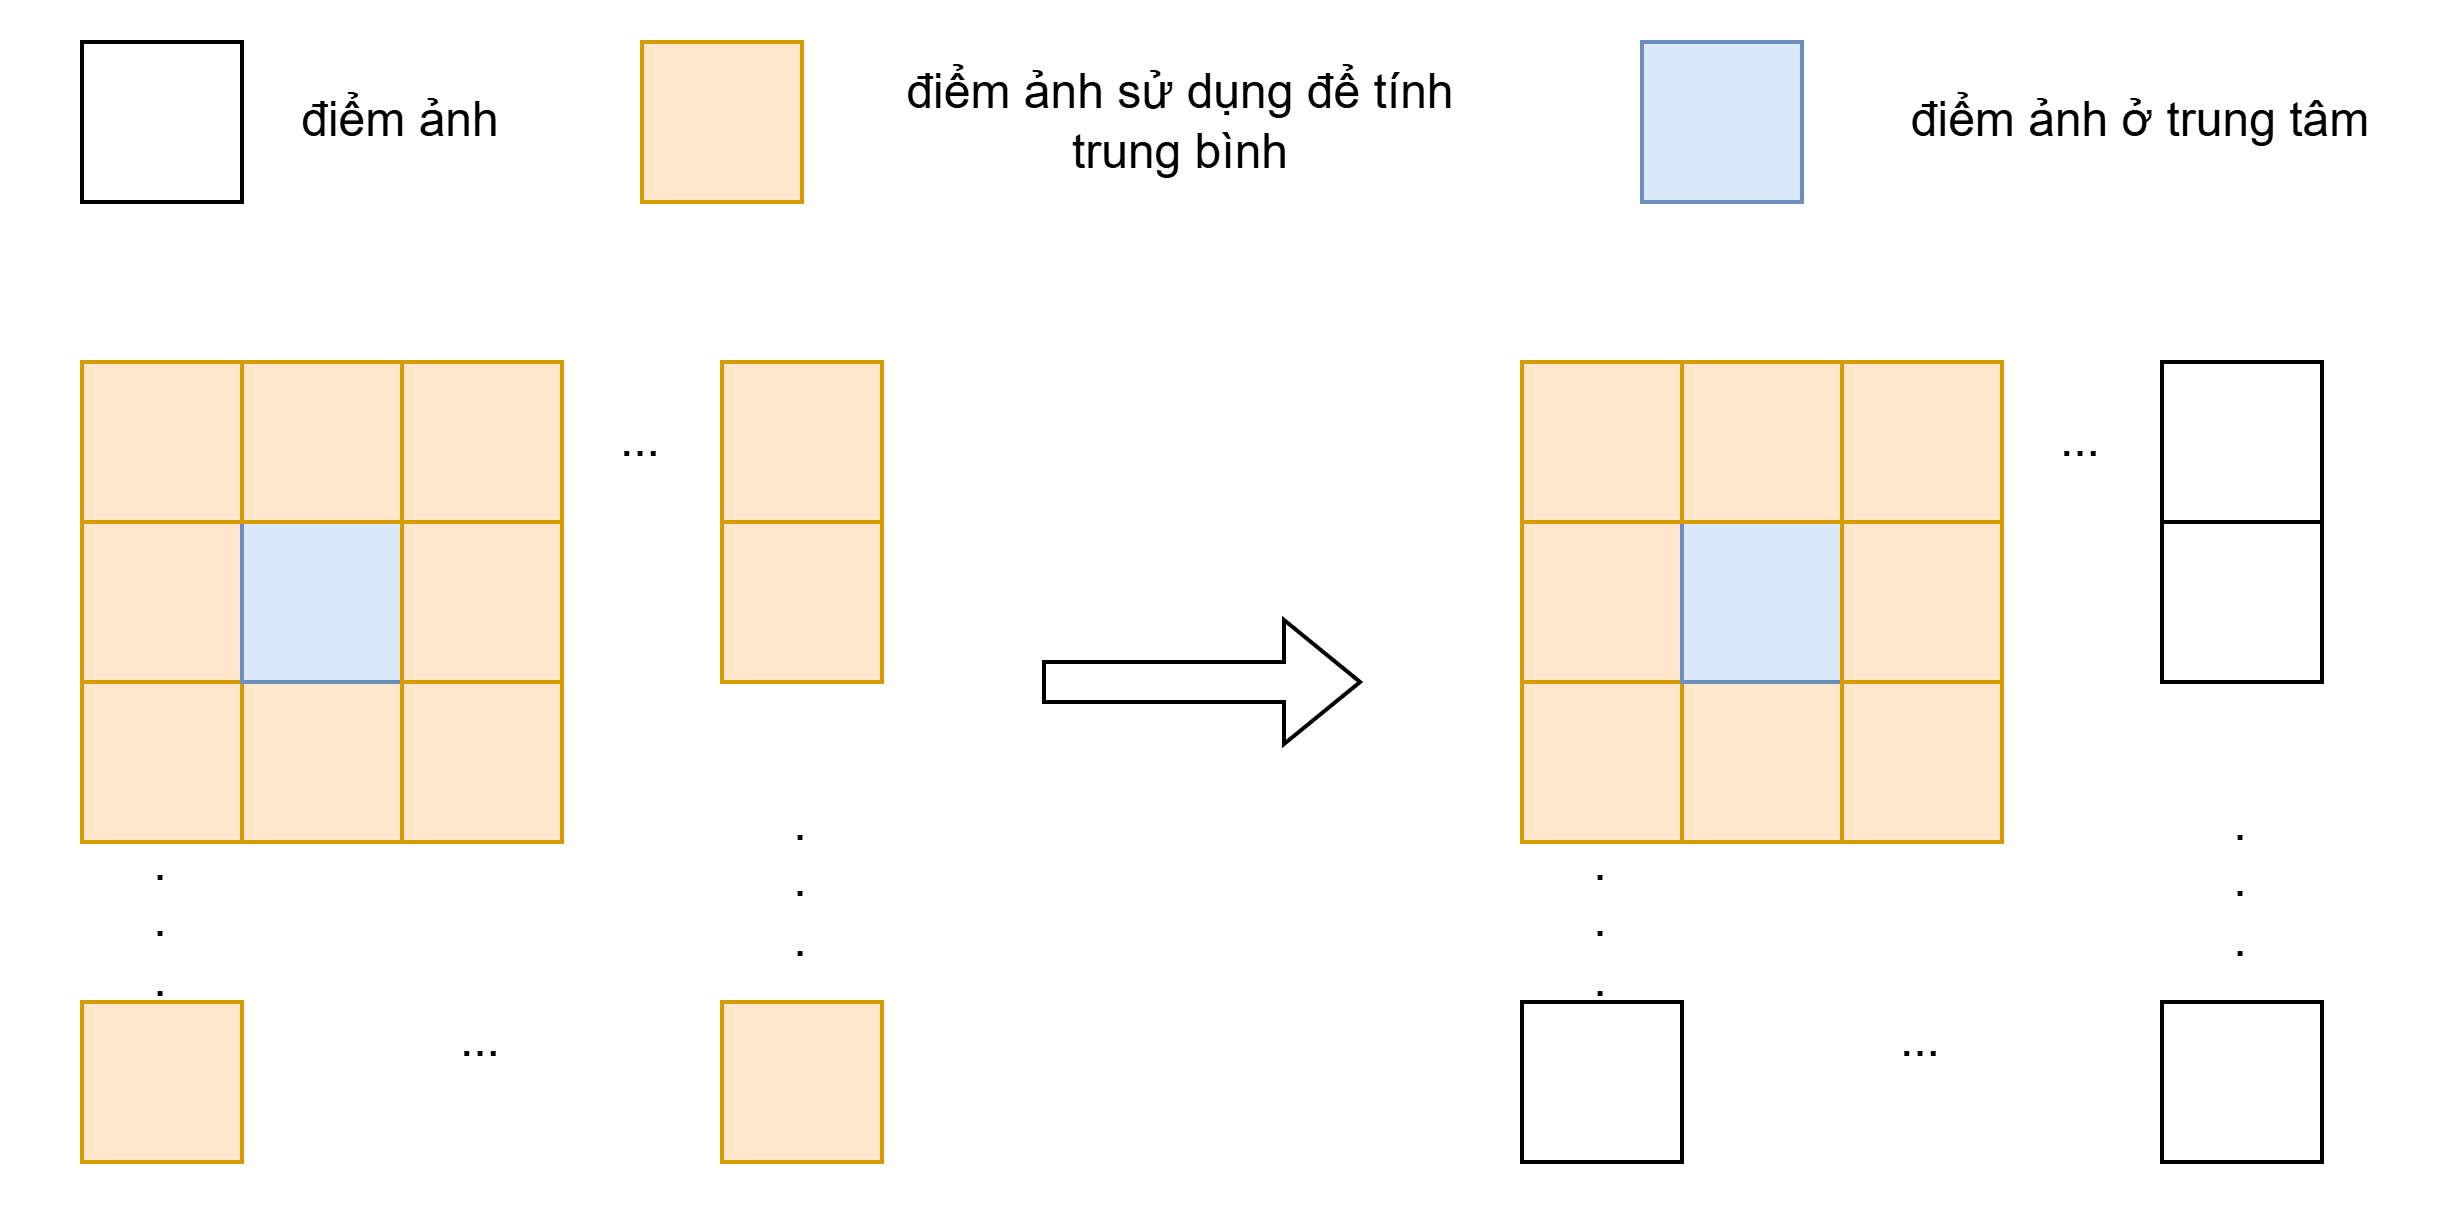
\includegraphics[width=\linewidth]{figures/ciOptimize.png}
	\caption{Phiên bản thiết kế phần cứng của biểu diễn điểm ảnh trung tâm - CI}
	\label{fig:ciOptimize}
\end{figure} 
Hình \ref{fig:ciOptimize} mô tả phiên bản phù hợp hơn của biểu diễn điểm ảnh trung tâm (CI) với việc thay đổi từ tính toán trung bình của toàn bộ bức ảnh thành tính toán trung bình của một vùng nội bộ trong bức ảnh. Điều này sẽ làm tăng tính xử lý thời gian thực của thiết kế lên vì không cần phải lưu lại toàn bộ bức ảnh. Kết quả nghiên cứu của Wang và Zhang \cite{realTimeTexture} đã cho thấy sự thay đổi về tính toán không gây ra sai số quá lớn về độ chính xác, giữ nguyên với Outex\_TC10 với, giảm 0.052\% với tập Outex\_TC12\_000 và giảm 0.104\% với tập Outex\_TC12\_002.

\subsection{Sơ đồ triển khai thuật toán}
Quá trình tạo ra biểu đồ histogram được mô tả theo hình \ref{fig:histogramStep}. Với đầu vào là ảnh kết cấu, sau quá trình lấy mẫu theo các công thức \ref{eq:relbp_ci_op}, \ref{eq:relbp_ni}, \ref{eq:relbp_rd} ta được các mô tả thô của ảnh. Sau đó, thực hiện một giai đoạn là "Joint Histogram", tại giai đoạn này, thực tế ta sẽ đếm xem là mô tả đấy xuất hiện bao nhiêu lần, do đó kết quả đạt được là một biểu đồ histogram. Sau đó ta sẽ nối lần lượt các biểu đồ này lại để được đặc trưng cuối cùng. 

\begin{figure} [!ht]
	\centering
	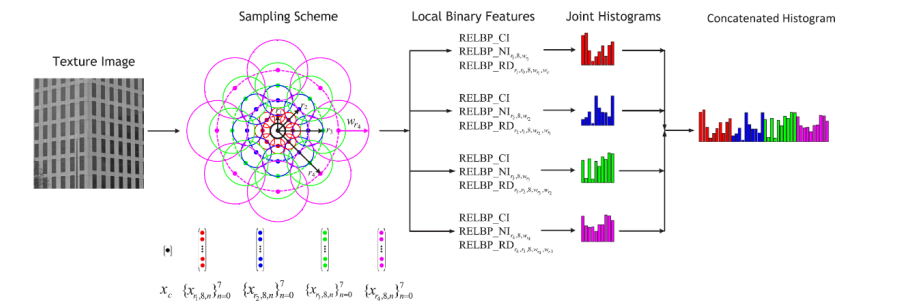
\includegraphics[width= 1\linewidth]{figures/histogramStep.png}
	\caption{Quá trình tạo ra đặc trưng của thuật toán RELBP \cite{realTimeTexture}}
	\label{fig:histogramStep}
\end{figure} 


\begin{figure} [!ht]
	\centering
	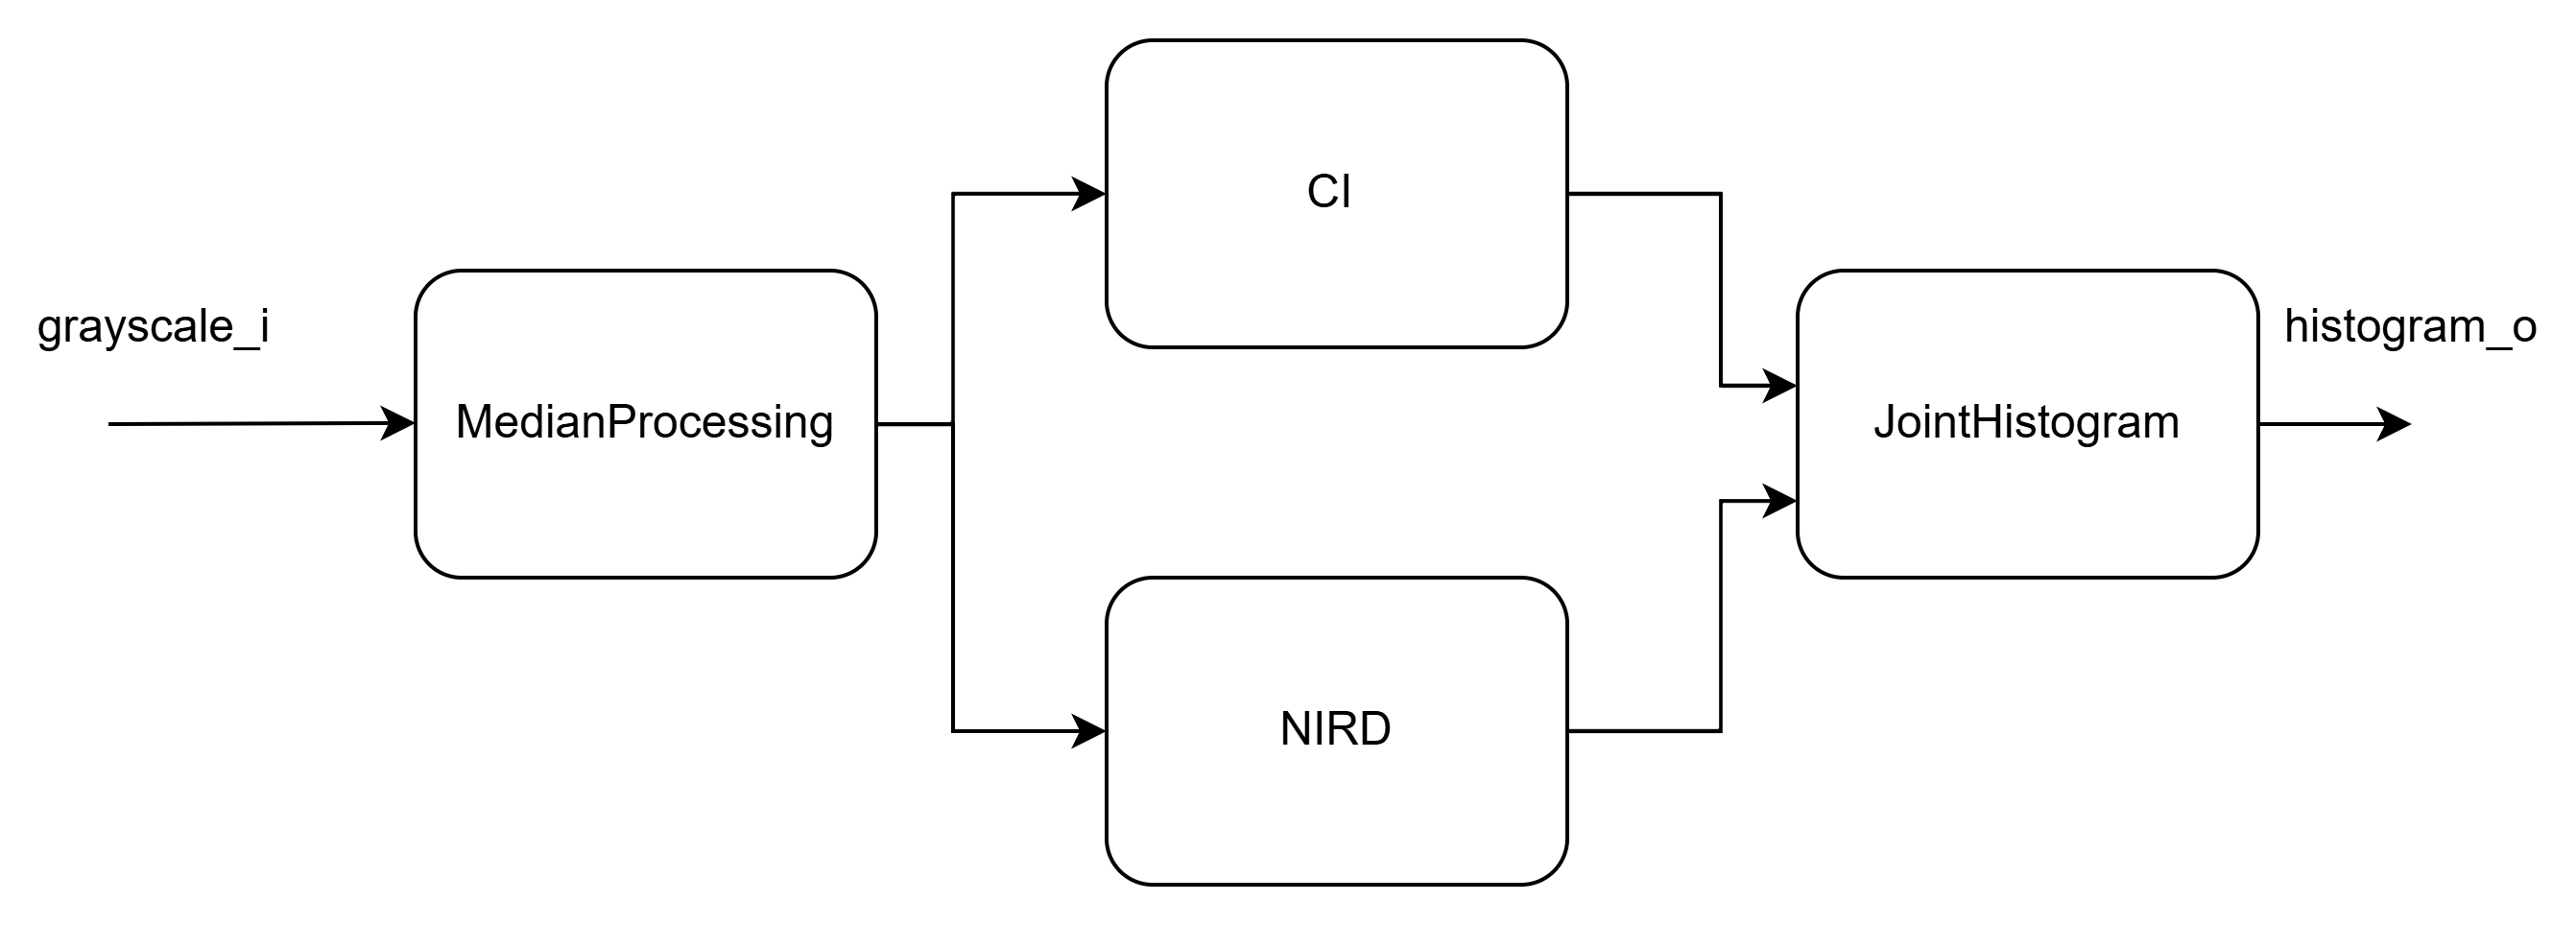
\includegraphics[width= 1\linewidth]{figures/fullArch.png}
	\caption{Sơ đồ kiến trúc tổng quát của MRELBP IP}
	\label{fig:fullArch}
\end{figure} 


Với những mô tả trên, sơ đồ thuật toán được đưa ra như hình \ref{fig:fullArch}. Một cách cụ thể hơn, vì MRELBP là phiên bản của RELBP với $\phi()$ là bộ tính trung vị, nên khi thiết kế phần cứng, ta sẽ đưa ra toàn bộ các phiên bản tính trung vị của ảnh đầu vào. Sau đó, sẽ có 2 bộ là CI và NIRD để tính các giá trị đặc trưng theo mô tả công thức \ref{eq:relbp_ci_op}, \ref{eq:relbp_ni}, \ref{eq:relbp_rd}. Vì NIRD có cách tính và yêu cầu đầu vào tương đối giống nhau, do đó, 2 mô tả này có thể xây dựng trong cùng 1 mô-đun để tiết kiệm tài nguyên. Sau đó 3 mô tả này sẽ thực hiện qua bước "JointHistogram" để đạt được đặc trưng đầu ra.


\section{ Đặc tả kỹ thuật}



\subsection{Đặc tả mô-đun MRELBP}

Bảng \ref{tab:paramListMRELBP}, \ref{tab:signalListMRELBP} mô tả các tham số và tín hiệu đầu vào, đầu ra của mô-đun MRELBP. 
\begin{table}[h]
    \centering
    \renewcommand{\arraystretch}{1.3} % Tăng khoảng cách dòng
        \caption{Danh sách các tham số của mô-đun MRELBP }
    \begin{tabular}{|p{3cm} p{4cm} p{8cm}|}
        \hline
        \rowcolor{gray!30}
        \textbf{Tham số } & \textbf{Giá trị mặc định}  & \textbf{Mô tả} \\
        \hline
        ROWS & 128 & Kích thước chiều cao của ảnh
        \\ \hline
        COLS & 128 & Kích thước chiều rộng của ảnh
        \\ \hline
    \end{tabular}

    \label{tab:paramListMRELBP}
\end{table}

\begin{table}[h]
    \centering
    \renewcommand{\arraystretch}{1.3} % Tăng khoảng cách dòng
        \caption{Danh sách các tín hiệu của giao diện mô-đun MRELBP}
    \begin{tabular}{|p{3cm} p{2cm} p{2cm} p{8cm}|}
        \hline
        \rowcolor{gray!30}
        \textbf{Tên tín hiệu} & \textbf{Độ rộng} & \textbf{Vào ra} & \textbf{Mô tả} \\
        \hline
        clk & 1 & Vào & Tín hiệu clock \\
        \hline
        rst\_n & 1 & Vào & Reset đồng bộ, kích hoạt mức thấp \\
        \hline
        start\_i & 1 & Vào & Tín hiệu bắt đầu (liên quan đến đầu ra)
        \\ \hline
        grayscale\_i & 8 & Vào & Dữ liệu điểm ảnh 
        \\ \hline
        i\_valid & 1 & Vào & Tín hiệu báo hiệu dữ liệu đầu vào là hợp lệ
        \\ \hline
        o\_data\_ready & 1 & Ra & Tín hiệu thông báo sẵn sàng cho đầu ra
        \\ \hline
        histogram\_o & 32 & Ra & Đặc trưng histogram
        \\ \hline
        o\_valid & 1 & Ra & Tín hiệu báo hiệu dữ liệu đầu ra là hợp lệ
        \\ \hline
        i\_data\_ready & 1 & Vào & Tín hiệu thông báo sẵn sàng nhận dữ liệu
        \\ \hline
        o\_intr & 1 & Ra &Tín hiệu báo hiệu đã xử lý xong
        \\ \hline
    \end{tabular}

    \label{tab:signalListMRELBP}
\end{table}


Hình \ref{fig:mrelbpArchitecture} mô tả sơ đồ khối của mô-đun MRELBP một cách chi tiết hơn. mô-đun \textbf{MedianProcessing} được cấu thành từ mô-đun Buffer6Rows, mô-đun ZeroPadding và mô-đun MedianCalculation. Dữ liệu đầu ra là giá trị trung vị của ảnh, sau đó sẽ đi đến các mô-đun sau là \textbf{CI} và \textbf{NIRD}. Mô tả chi tiết hơn về đường đi của dữ liệu sẽ được giới thiệu tại các phần sau.
\begin{figure} [!ht]
	\centering
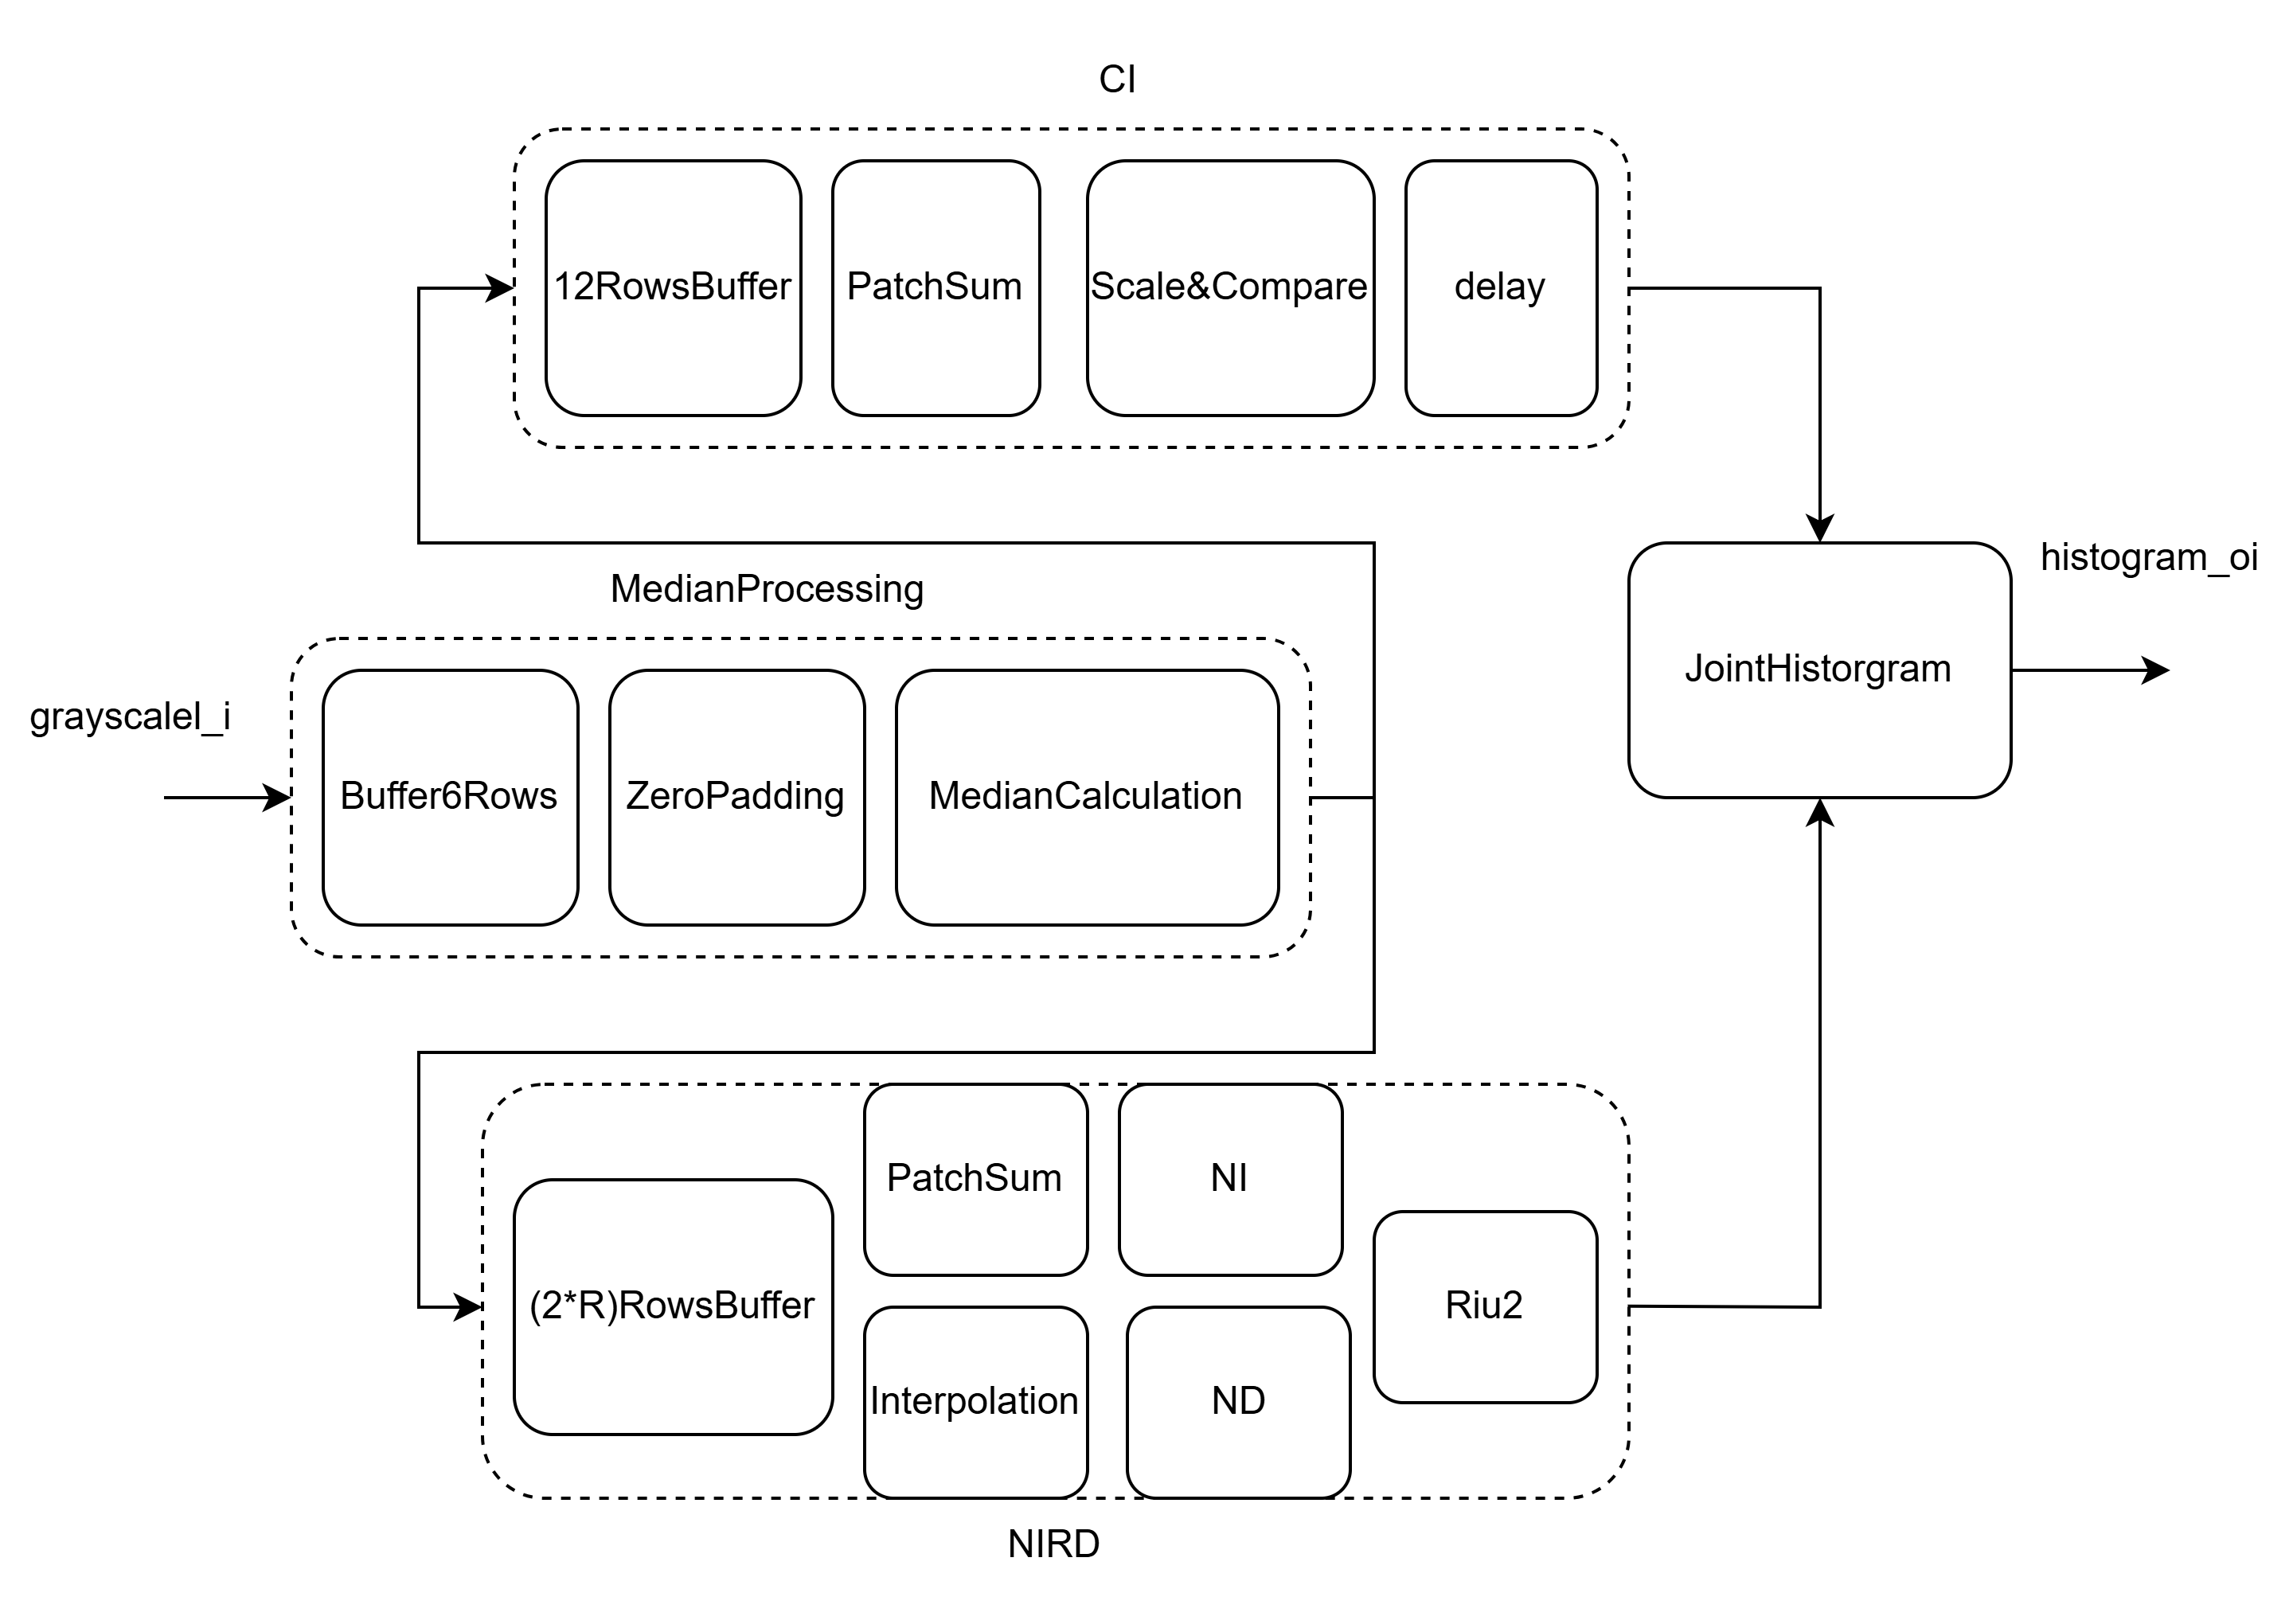
\includegraphics[width=1\linewidth]{figures/mrelbpArchitecture.png}
	\caption{Sơ đồ khối của mô-đun MRELBP}
	\label{fig:mrelbpArchitecture}
\end{figure}



\begin{figure} [!ht]
	\centering
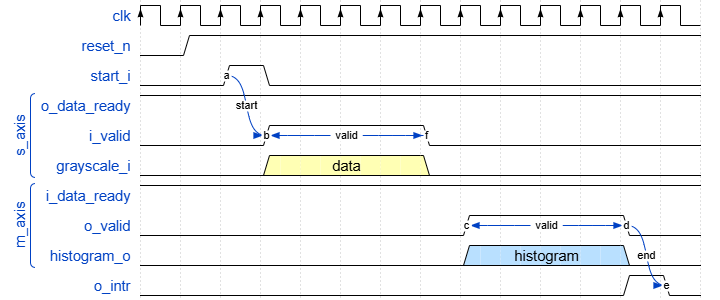
\includegraphics[width=1\linewidth]{figures/mrelbp.png}
	\caption{Dạng sóng của mô-đun MRELBP}
	\label{fig:mrelbpWaveform}
\end{figure}




\newpage
\subsection{Đặc tả mô-đun MedianProcessing}
Theo mô tả từ hình \ref{fig:mrelbpArchitecture} thì mô-đun MedianProcessing gồm 3 thành phần chính hay 3 mô-đun bao gồm \textbf{Buffer6Rows, ZeroPadding, MedianCalculation}. \textit{\textbf{Lưu ý}: Do mô-đun MedianProcessing sẽ tính giá trị trung vị ứng với 3 cửa sổ theo bán kính r, nên tại phần này sẽ mô tả một cách tổng quát từng mô-đun mà không chi tiết cụ thể theo từng giá trị r}.
\begin{table}[!ht]
    \centering
    \renewcommand{\arraystretch}{1.3} % Tăng khoảng cách dòng
        \caption{Tham số của mô-đun MedianProcessing}
    \begin{tabular}{|p{3cm} p{4cm} p{8cm}|}
        \hline
        \rowcolor{gray!30}
        \textbf{Tham số } & \textbf{Giá trị mặc định}  & \textbf{Mô tả} \\
        \hline
        COLS & 128 & Kích thước độ rộng của ảnh
        \\ \hline
        ROWS & 128 & Kích thước chiều cao của ảnh
        \\
        \hline
    \end{tabular}

    \label{tab:paramListMedianProcessing}
\end{table}

\begin{table}[!ht]
    \centering
    \renewcommand{\arraystretch}{1.3} % Tăng khoảng cách dòng
        \caption{Danh sách các tín hiệu của mô-đun MedianProcessing}
    \begin{tabular}{|p{3cm} p{2cm} p{2cm} p{8cm}|}
        \hline
        \rowcolor{gray!30}
        \textbf{Tên tín hiệu} & \textbf{Độ rộng} & \textbf{Vào ra} & \textbf{Mô tả} \\
        \hline
        clk & 1 & Vào & Tín hiệu clock \\
        \hline
        rst\_n & 1 & Vào & Reset đồng bộ, kích hoạt mức thấp \\
        \hline 
        data\_i & 8 & Vào & Dữ liệu điểm ảnh đầu vào
        \\ \hline
        i\_valid & 1 & Vào & Tín hiệu thông báo giá trị đầu vào là hợp lệ
        \\ \hline
        data\_o & 8 & Ra & Dữ liệu điểm ảnh đầu ra gốc
        \\ \hline
        o\_valid & 1 & Ra & Tín hiệu thông báo dữ liệu đầu ra gốc là hợp lệ
        \\ \hline
        m\_3x3\_o & 8 & Ra & Giá trị trung vị của cửa sổ 3x3
        \\ \hline
        o\_3x3\_valid & 1 & Ra & Tín hiệu thông báo dữ liệu trung vị 3x3 hợp lệ
                \\ \hline
        m\_5x5\_o & 8 & Ra & Giá trị trung vị của cửa sổ 5x5
        \\ \hline
        o\_5x5\_valid & 1 & Ra & Tín hiệu thông báo dữ liệu trung vị 5x5 hợp lệ
                \\ \hline
        m\_7x7\_o & 8 & Ra & Giá trị trung vị của cửa sổ 7x7
        \\ \hline
        o\_7x7\_valid & 1 & Ra & Tín hiệu thông báo dữ liệu trung vị 7x7 hợp lệ
        \\ \hline
       
    \end{tabular}

    \label{tab:signalListMedianProcessing}
\end{table}

\begin{figure}[!ht]
    \centering
    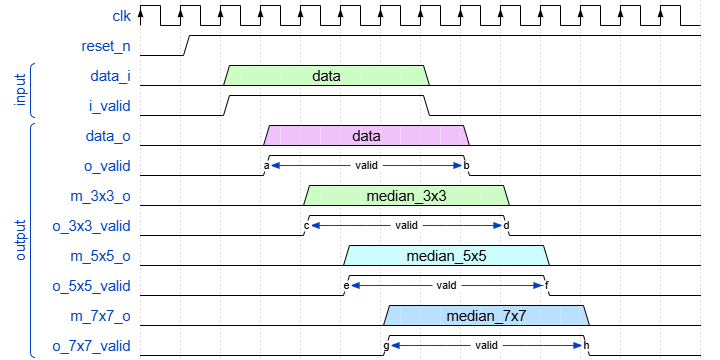
\includegraphics[width=1\linewidth, height =7cm]{figures/medianProcessing.png}
    \caption{Dạng sóng của mô-đun MedianProcessing}
    \label{fig:medianProcessing}
\end{figure}
\subsubsection{Đặc tả mô-đun Buffer6Rows}
mô-đun Buffer6Rows là tập hợp của \textbf{6} mô-đun LineBuffer tạo thành, cụ thể được mô tả trong hình \ref{fig:buffer6RowsAr}. Do đó, để mô tả đặc tả cho mô-đun Buffer6Rows, ta sẽ đi từ mô-đun LineBuffer. mô-đun LineBuffer là mô-đun cơ sở để xây dựng lên các mô-đun lớn hơn như Buffer6Rows. Chức năng của mô-đun này là đệm dữ liệu theo từng hàng để thuận tiện cho việc định dạng dữ liệu cho các mô-đun đứng sau.

\begin{figure}[!ht]
    \centering
    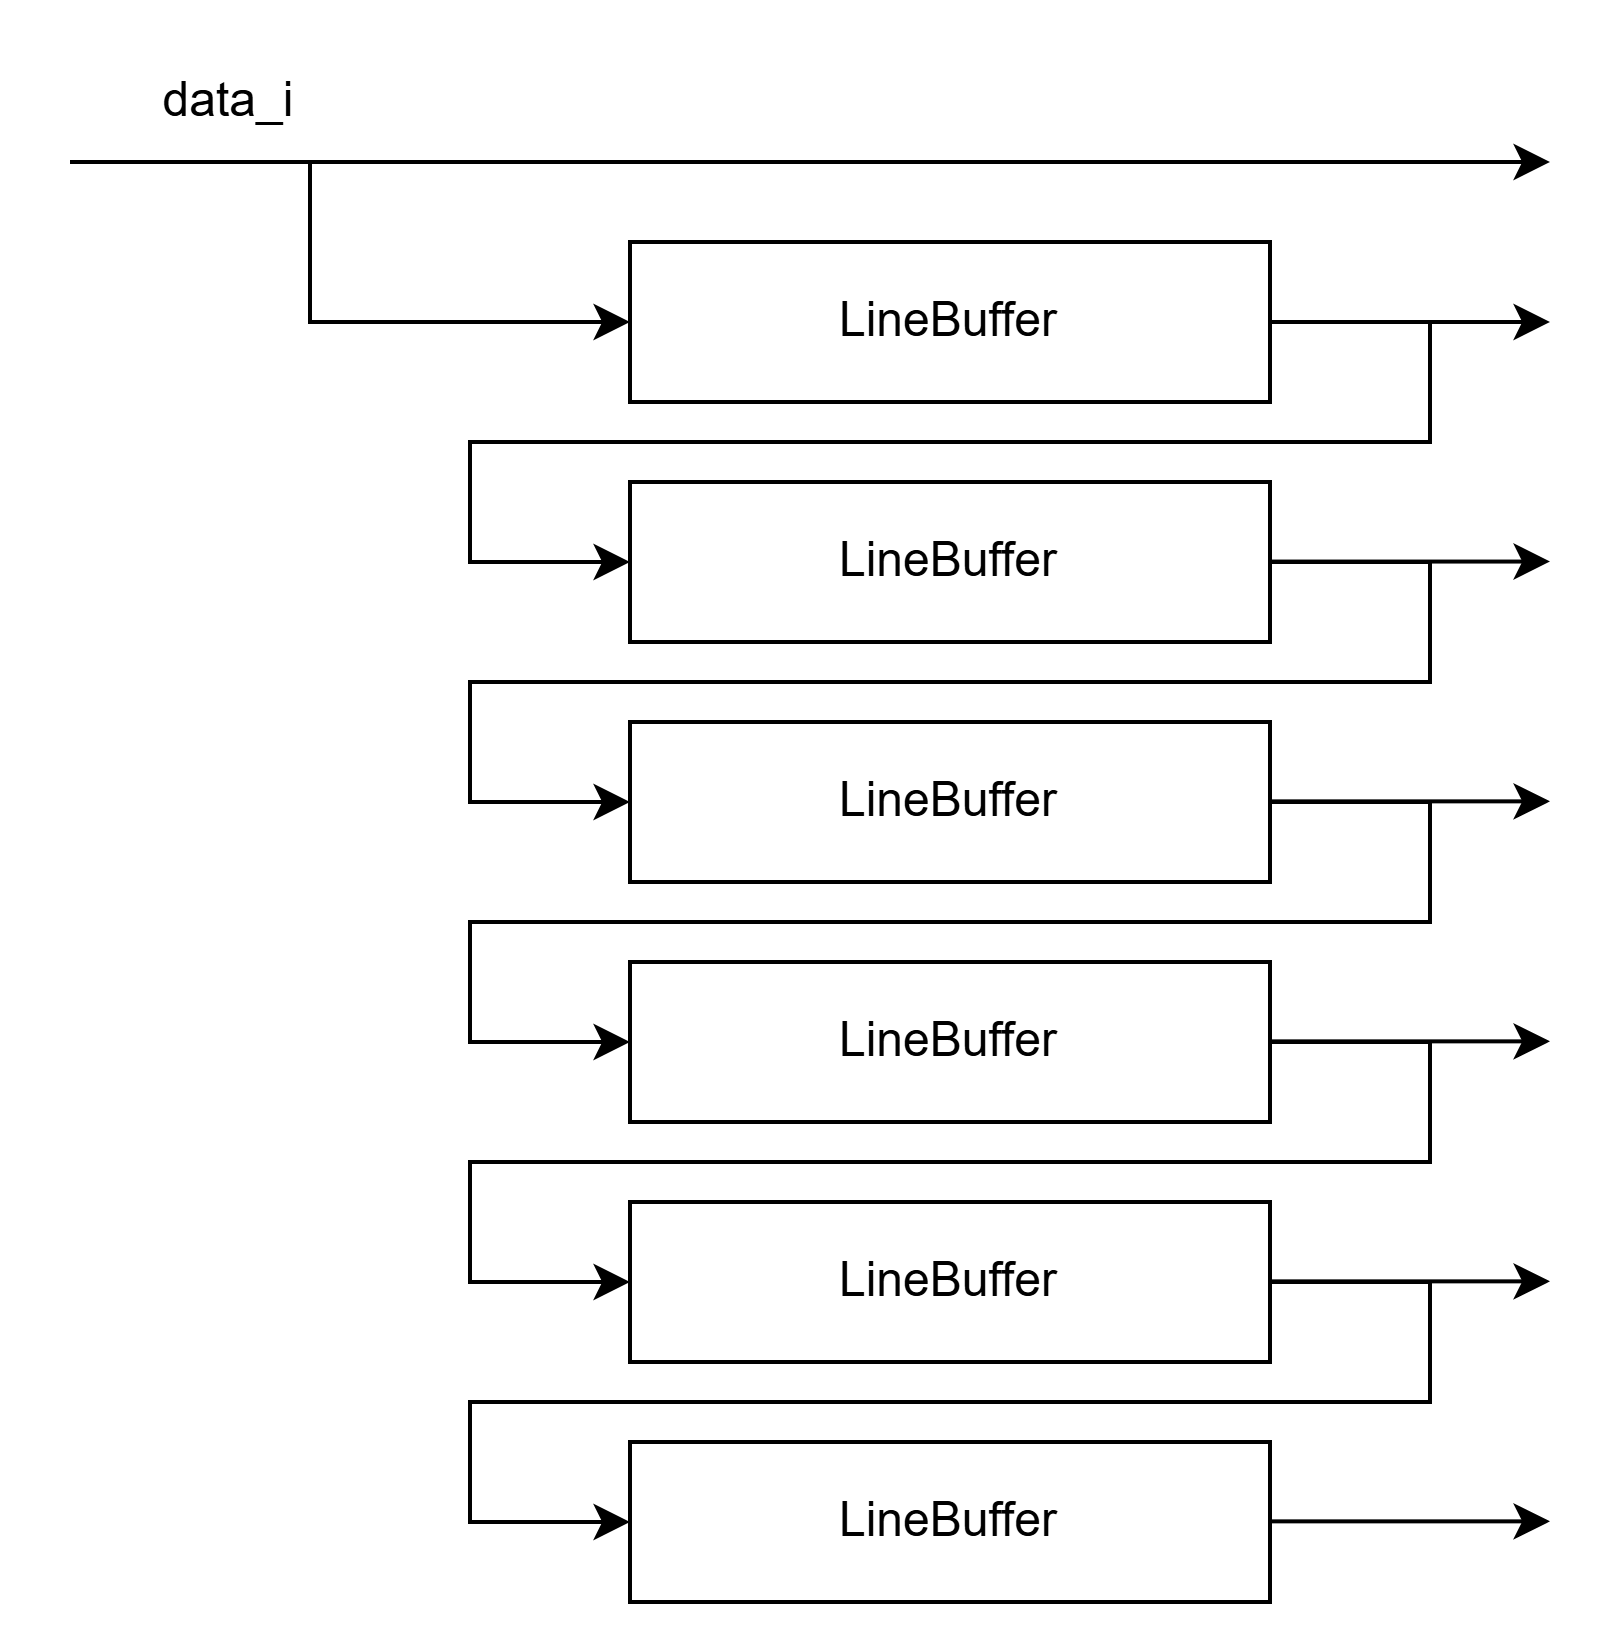
\includegraphics[width=1\linewidth]{figures/buffer6RowsAr.png}
    \caption{Sơ đồ khối của mô-đun Buffer6Rows}
    \label{fig:buffer6RowsAr}
\end{figure}


\begin{table}[!ht]
    \centering
    \renewcommand{\arraystretch}{1.3} % Tăng khoảng cách dòng
        \caption{Danh sách các tham số của mô-đun LineBuffer }
    \begin{tabular}{|p{3cm} p{4cm} p{8cm}|}
        \hline
        \rowcolor{gray!30}
        \textbf{Tham số } & \textbf{Giá trị mặc định}  & \textbf{Mô tả} \\
        \hline
        DEPTH & 128 & Kích thước độ rộng của ảnh
        \\ \hline
    \end{tabular}

    \label{tab:paramListLineBuffer}
\end{table}


\begin{table}[h]
    \centering
    \renewcommand{\arraystretch}{1.3} % Tăng khoảng cách dòng
        \caption{Danh sách các tín hiệu của giao diện mô-đun LineBuffer}
    \begin{tabular}{|p{3cm} p{2cm} p{2cm} p{8cm}|}
        \hline
        \rowcolor{gray!30}
        \textbf{Tên tín hiệu} & \textbf{Độ rộng} & \textbf{Vào ra} & \textbf{Mô tả} \\
        \hline
        clk & 1 & Vào & Tín hiệu clock \\
        \hline
        rst\_n & 1 & Vào & Reset đồng bộ, kích hoạt mức thấp \\
        \hline
        i\_valid & 1 & Vào & Tín hiệu thông báo dữ liệu đầu vào là hợp lệ
        \\ \hline
        data\_i & 8 & Vào & Dữ liệu đầu vào
        \\ \hline
        data\_o & 8 & Ra & Dữ liệu đầu ra
        \\ \hline
        o\_start & 1& Ra & Tín hiệu thông báo bắt đầu có dữ liệu đầu ra
        \\ \hline
        o\_valid & 1& Ra & Tín hiệu thông báo dữ liệu đầu là hợp lệ
        \\ \hline
        o\_finish & 1 & Ra & Tín hiệu thông báo kết thúc đệm dữ liệu        
        \\ \hline
    \end{tabular}

    \label{tab:signalListLineBuffer}
\end{table}
\begin{figure}[!ht]
    \centering
    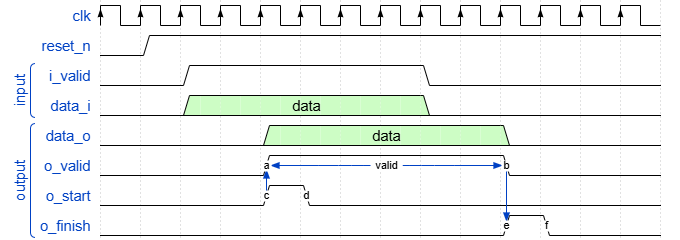
\includegraphics[width=1\linewidth]{figures/lineBuffer.png}
    \caption{Dạng sóng của mô-đun LineBuffer}
    \label{fig:lineBuffer}
\end{figure}
\begin{figure}[H]
    \centering
    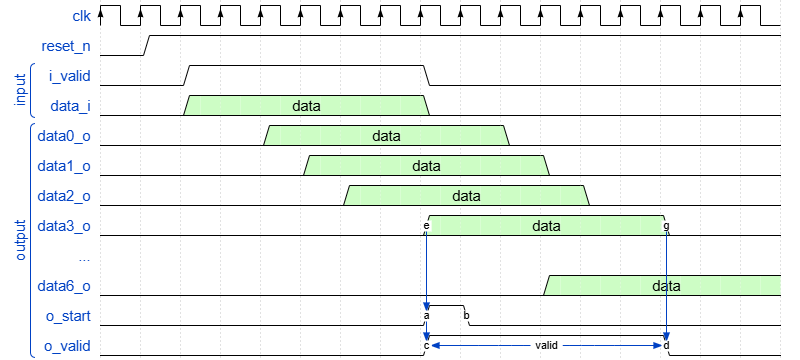
\includegraphics[width=1\linewidth]{figures/Buffer6Rows.png}
    \caption{Dạng sóng của mô-đun Buffer6Rows}
    \label{fig:Buffer6Rows}
\end{figure}

\subsubsection{Đặc tả mô-đun ZeroPadding}
Đệm 0 là một kỹ thuật được sử dụng để thêm hàng và cột vào rìa bức ảnh, mục đích để khi xử lý với một số kỹ thuật như nhân chập, kích thước đầu ra sẽ không bị thay đổi so với đầu vào \textit{(danh sách tín hiệu sẽ có mô tả chung về số lượng đầu vào\&ra vì các tín hiệu cửa mô-đun sẽ thuộc vào kích thước cửa sổ, xem thêm ở phần RTL của ZeroPadding).}




\begin{table}[!ht]
    \centering
    \renewcommand{\arraystretch}{1.3} % Tăng khoảng cách dòng
        \caption{Danh sách các tham số của mô-đun ZeroPadding }
    \begin{tabular}{|p{3cm} p{4cm} p{8cm}|}
        \hline
        \rowcolor{gray!30}
        \textbf{Tham số } & \textbf{Giá trị mặc định}  & \textbf{Mô tả} \\
        \hline
        COLS & 128 & Kích thước độ rộng của ảnh
        \\ \hline
        ROWS & 128 & Kích thước độ cao của ảnh
        \\ \hline
    \end{tabular}

    \label{tab:paramListZeroPadding}
\end{table}


\begin{table}[h]
    \centering
    \renewcommand{\arraystretch}{1.3} % Tăng khoảng cách dòng
        \caption{Danh sách các tín hiệu của giao diện mô-đun ZeroPadding}
    \begin{tabular}{|p{3cm} p{2cm} p{2cm} p{8cm}|}
        \hline
        \rowcolor{gray!30}
        \textbf{Tên tín hiệu} & \textbf{Độ rộng} & \textbf{Vào ra} & \textbf{Mô tả} \\
        \hline
        clk & 1 & Vào & Tín hiệu clock \\
        \hline
        rst\_n & 1 & Vào & Reset đồng bộ, kích hoạt mức thấp \\
        \hline
        i\_valid & 1 & Vào & Tín hiệu thông báo dữ liệu đầu vào là hợp lệ
        \\ \hline
        d0\_i & 8 & Vào & Dữ liệu đầu vào
        \\ \hline
        d1\_i & 8 & Vào & Dữ liệu đầu vào
        \\
        \hline
        \multicolumn{4}{|c|}{Tùy thuộc vào kích thước cửa sổ, 3x3 thì sẽ có 3 đầu vào, 5x5 có 5 đầu vào, 7x7 có 7 đầu vào}
        \\ \hline
        d0\_o & 8 & Ra & Dữ liệu đầu ra
        \\ \hline
        d1\_o & 8 & Ra & Dữ liệu đầu ra
        \\ \hline
                \multicolumn{4}{|c|}{Tùy thuộc vào kích thước cửa sổ, 3x3 thì sẽ có 9 đầu ra, 5x5 có 25 đầu ra, 7x7 có 49 đầu ra}
        \\ \hline
        o\_valid & 1& Ra & Tín hiệu thông báo dữ liệu đầu là hợp lệ
        \\ \hline
    \end{tabular}

    \label{tab:signalListZeroPadding}
\end{table}

\begin{figure}[!ht]
    \centering
    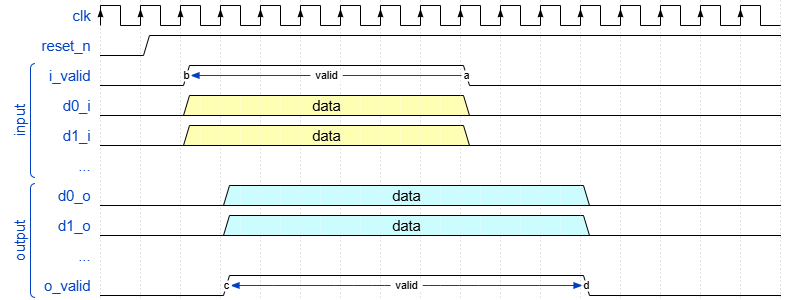
\includegraphics[width=\linewidth]{figures/zeroPadding.png}
    \caption{Dạng sóng của mô-đun ZeroPadding}
    \label{fig:zeroPadding}
\end{figure}


\subsubsection{Đặc tả mô-đun MedianCalculation}
Vì kiến trúc của mô-đun MedianCalculation sẽ phụ thuộc vào từng loại cửa sổ, tức là cửa sổ 3x3 sẽ có cách tính khác cửa sổ 5x5, nên để thuận lợi cho việc mô tả, sinh viên sẽ mô tả theo 1 giao diện chung mà số lượng các cổng sẽ khác đối với từng loại cửa sổ. Cụ thể hơn sẽ được mô tả tại thiết kế RTL cho mô-đun MedianCalculation
\begin{table}[!ht]
    \centering
    \renewcommand{\arraystretch}{1.3} % Tăng khoảng cách dòng
        \caption{Danh sách các tham số của mô-đun MedianCalculation}
    \begin{tabular}{|p{3cm} p{4cm} p{8cm}|}
        \hline
        \rowcolor{gray!30}
        \textbf{Tham số } & \textbf{Giá trị mặc định}  & \textbf{Mô tả} \\
        \hline
        COLS & 128 & Kích thước độ rộng của ảnh
        \\ \hline
        ROWS & 128 & Kích thước độ cao của ảnh
        \\ \hline
    \end{tabular}

    \label{tab:paramListMedianCalculation}
\end{table}


\begin{table}[h]
    \centering
    \renewcommand{\arraystretch}{1.3} % Tăng khoảng cách dòng
        \caption{Danh sách các tín hiệu của giao diện mô-đun MedianCalculation}
    \begin{tabular}{|p{3cm} p{2cm} p{2cm} p{8cm}|}
        \hline
        \rowcolor{gray!30}
        \textbf{Tên tín hiệu} & \textbf{Độ rộng} & \textbf{Vào ra} & \textbf{Mô tả} \\
        \hline
        clk & 1 & Vào & Tín hiệu clock \\
        \hline
        rst\_n & 1 & Vào & Reset đồng bộ, kích hoạt mức thấp \\
        \hline
        i\_valid & 1 & Vào & Tín hiệu thông báo dữ liệu đầu vào là hợp lệ
        \\ \hline
        S0\_i & 8 & Vào & Dữ liệu đầu vào
        \\ \hline
        S1\_i & 8 & Vào & Dữ liệu đầu vào
        \\
        \hline
        \multicolumn{4}{|c|}{Tùy thuộc vào kích thước cửa sổ, 3x3 thì sẽ có 9 đầu vào, 5x5 có 25 đầu vào, 7x7 có 49 đầu vào}
        \\ \hline
        median\_o & 8 & Ra & Dữ liệu đầu ra
        \\ \hline
        o\_valid & 1& Ra & Tín hiệu thông báo dữ liệu đầu là hợp lệ
        \\ \hline
    \end{tabular}

    \label{tab:signalListMedianCalculation}
\end{table}

\begin{figure}[!ht]
    \centering
    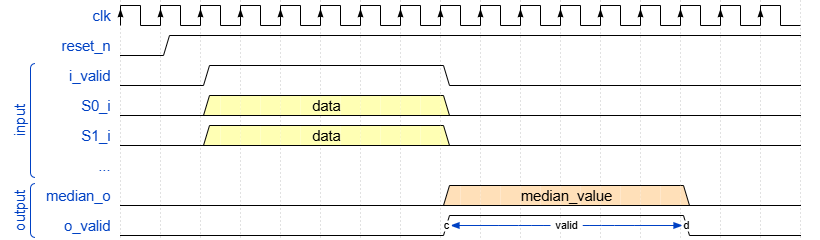
\includegraphics[width=\linewidth]{figures/medianCalculation.png}
    \caption{Dạng sóng của mô-đun MedianCalculation}
    \label{fig:medianCalculation}
\end{figure}
\subsection{Đặc tả mô-đun CI}
Bảng \ref{tab:paramListCI}, \ref{tab:signalListCI} mô tả các tham số và tín hiệu đầu vào, đầu ra của mô-đun CI.

\begin{table}[!ht]
    \centering
    \renewcommand{\arraystretch}{1.3} % Tăng khoảng cách dòng
        \caption{Tham số của mô-đun CI}
    \begin{tabular}{|p{3cm} p{4cm} p{8cm}|}
        \hline
        \rowcolor{gray!30}
        \textbf{Tham số } & \textbf{Giá trị mặc định}  & \textbf{Mô tả} \\
        \hline
        COLS & 128 & Kích thước độ rộng của ảnh
        \\ \hline
        ROWS & 128 & Kích thước chiều cao của ảnh
        \\
        \hline
    \end{tabular}

    \label{tab:paramListCI}
\end{table}

\begin{table}[!ht]
    \centering
    \renewcommand{\arraystretch}{1.3} % Tăng khoảng cách dòng
        \caption{Danh sách các tín hiệu của mô-đun CI}
    \begin{tabular}{|p{3cm} p{2cm} p{2cm} p{8cm}|}
        \hline
        \rowcolor{gray!30}
        \textbf{Tên tín hiệu} & \textbf{Độ rộng} & \textbf{Vào ra} & \textbf{Mô tả} \\
        \hline
        clk & 1 & Vào & Tín hiệu clock \\
        \hline
        rst\_n & 1 & Vào & Reset đồng bộ, kích hoạt mức thấp \\
        \hline 
        m\_3x3\_i & 8 & Vào & Dữ liệu trung vị của cửa sổ 3x3
        \\ \hline
        ci\_r2\_o & 1 & Ra & Mô tả ci đầu ra ứng với r = 2
        \\ \hline
        r2\_valid & 1 & Ra & Tín hiệu thông báo ci ứng với r = 2 là hợp lệ
        \\ \hline
        r2\_finish & 1 & Ra & Tín hiệu thông báo đã kết thúc quá trình tính ci ứng với r = 2
        \\ \hline
                ci\_r4\_o & 1 & Ra & Mô tả ci đầu ra ứng với r = 4
        \\ \hline
        r4\_valid & 1 & Ra & Tín hiệu thông báo ci ứng với r = 4 là hợp lệ
        \\ \hline
        r4\_finish & 1 & Ra & Tín hiệu thông báo đã kết thúc quá trình tính ci ứng với r = 4
        \\ \hline
                ci\_r6\_o & 1 & Ra & Mô tả ci đầu ra ứng với r = 6
        \\ \hline
        r6\_valid & 1 & Ra & Tín hiệu thông báo ci ứng với r = 6 là hợp lệ
        \\ \hline
        r6\_finish & 1 & Ra & Tín hiệu thông báo đã kết thúc quá trình tính ci ứng với r = 6
        \\ \hline
       
    \end{tabular}

    \label{tab:signalListCI}
\end{table}

\begin{figure}[!ht]
    \centering
    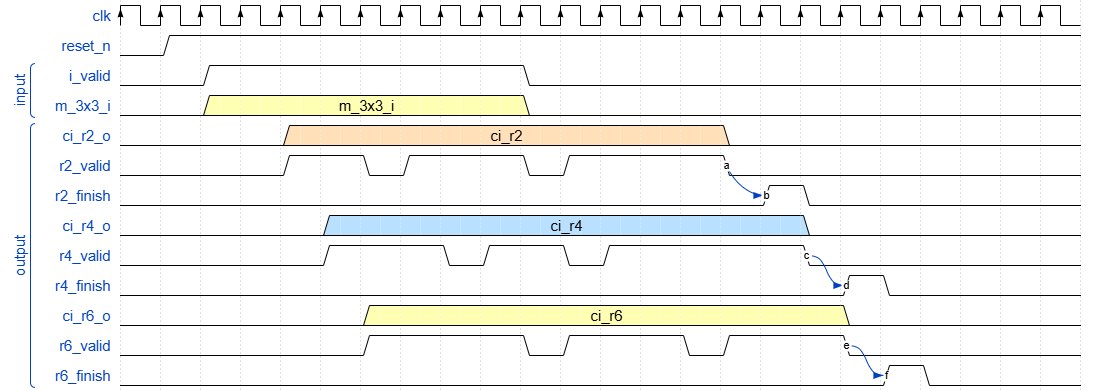
\includegraphics[width=\linewidth]{figures/ci.png}
    \caption{Dạng sóng của mô-đun CI}
    \label{fig:ci}
\end{figure}

Hình \ref{fig:ciArch} mô tả kiến trúc tổng quát của mô-đun CI. Sau khi giá trị trung vị tính từ cửa sổ 3x3 được tính xong sẽ đưa vào mô-đun này. Trong đây sẽ cần một bộ 12RowsBuffer để đệm dữ liệu nhằm tạo cửa sổ cho khối sau sử dụng với kích thước là (2*r+1, 2*r+1), vì r = 6 nên cửa sổ lớn nhất là 13x13, do đó nên cần đệm 12 hàng. Dữ liệu sau khi đệm sẽ đưa vào một khối gọi là "PatchSum", khối này có nhiệm vụ ghép dữ liệu thành một cửa sổ, sử dụng kĩ thuật cửa sổ trượt để tính tổng của cửa sổ và đầu ra sẽ bao gồm tổng và giá trị ở giữa của cửa sổ. Sau đó khối compare là mạch logic tổ hợp có thể so sánh và đưa ra giá trị CI ứng với cửa sổ đang được tính. Hình \ref{fig:mrelbpArchitecture} có mô tả thêm khối \textbf{"delay"}, thì khối này thực tế để làm trễ dữ liệu CI đầu ra để đồng bộ với NIRD, thực tế nó là các thanh ghi dịch, do đó sẽ không trình bày phần delay này. mô-đun 12RowsBuffer có nguyên tắc hoạt động tương tự với mô-đun Buffer6Rows. Phần gộp vào giữa PatchSum và khối logic tổ hợp gọi là \textit{MRELBP\_CI}. 

\begin{figure}[!ht]
    \centering
    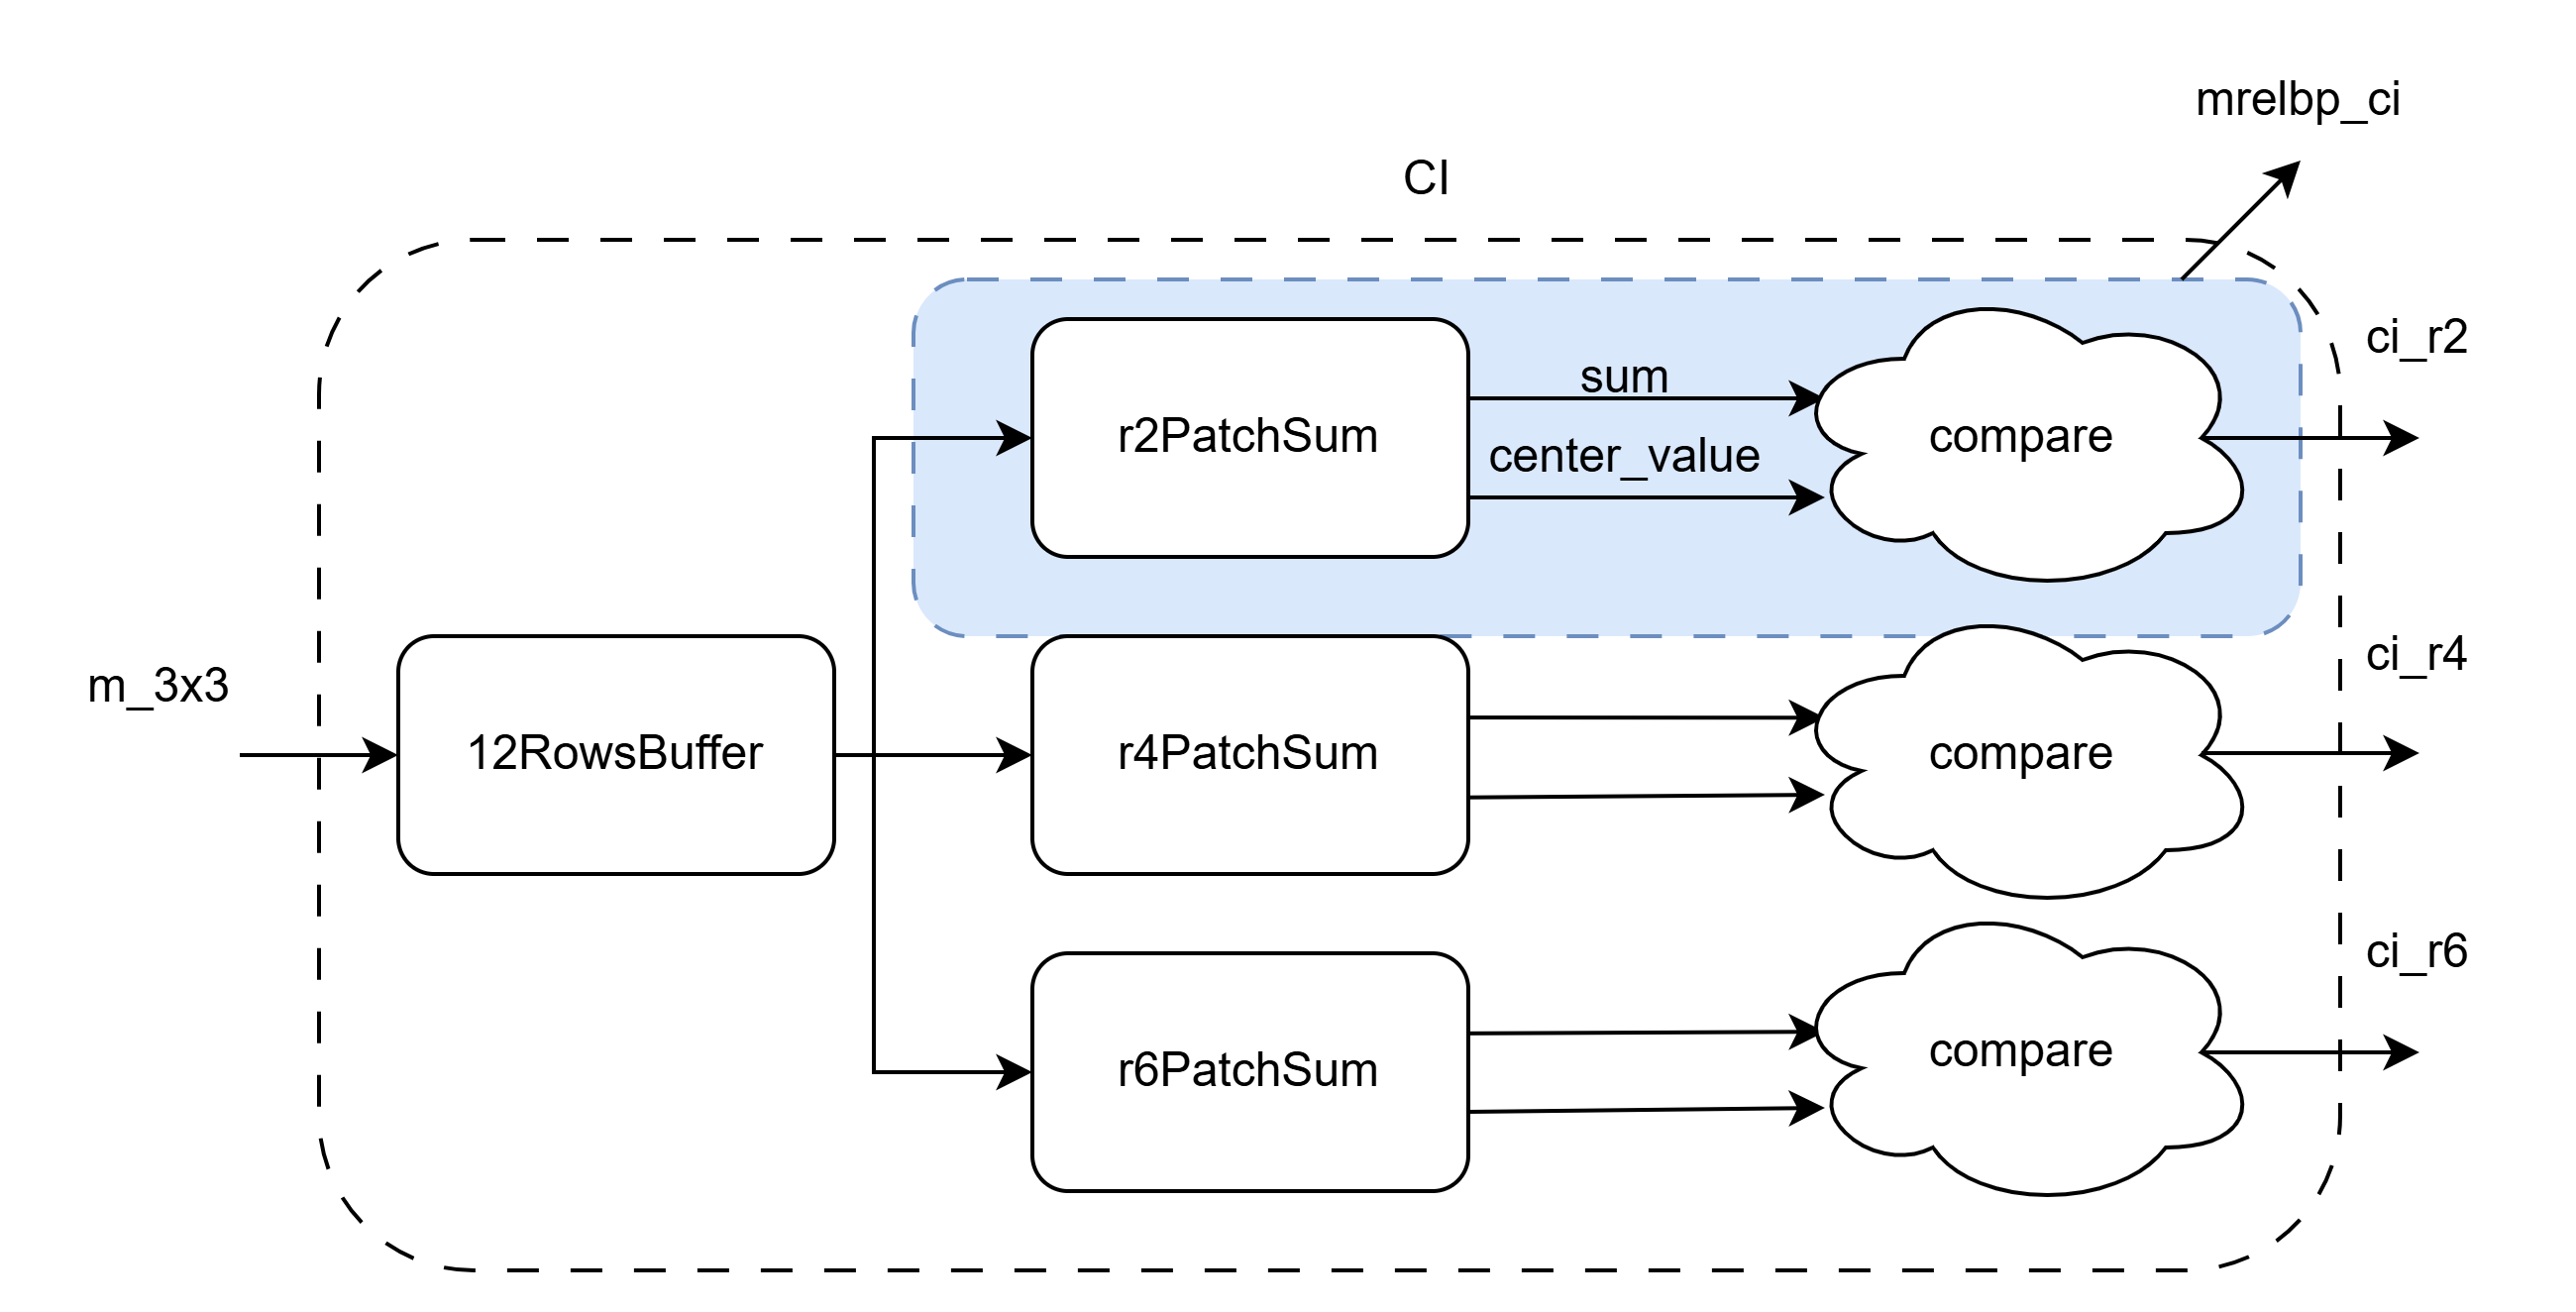
\includegraphics[width=\linewidth]{figures/ciArch.png}
    \caption{Sơ đồ khối của mô-đun CI}
    \label{fig:ciArch}
\end{figure}

\subsubsection{Đặc tả mô-đun MRELBP\_CI}
Bảng \ref{tab:paramListCICAL}, \ref{tab:signalListCICAL} mô tả về giao diện kết nối của mô-đun MRELBP\_CI. Với mô-đun này, sẽ được thiết kế theo nhiều giá trị r, ứng với đó thì sẽ có số lượng đầu vào khác nhau. Đầu ra gồm tín hiệu ci\_o, tín hiệu này chỉ có 1-bit ứng với 2 giá trị có thể có là 0 hoặc 1. Theo hình \ref{fig:ciArch}, bên trong mô-đun này sẽ có mô-đun \textit{PatchSum} để tính toán tổng của các điểm ảnh trong cửa sổ và sau đó là một khối logic tổ hợp để so sánh giá trị của \textbf{sum} và \textbf{center\_value} tương ứng với tổng của cửa sổ và điểm ảnh nằm giữa của cửa sổ. Chi tiết hơn sẽ được mô tả tại thiết kế RTL của mô-đun MRELBP\_CI. 


\begin{table}[!ht]
    \centering
    \renewcommand{\arraystretch}{1.3} % Tăng khoảng cách dòng
        \caption{Tham số của mô-đun MRELBP\_CI}
    \begin{tabular}{|p{3cm} p{4cm} p{8cm}|}
        \hline
        \rowcolor{gray!30}
        \textbf{Tham số } & \textbf{Giá trị mặc định}  & \textbf{Mô tả} \\
        \hline
        COLS & 128 & Kích thước độ rộng của ảnh
        \\ \hline
        ROWS & 128 & Kích thước chiều cao của ảnh
        \\
        \hline
    \end{tabular}

    \label{tab:paramListCICAL}
\end{table}
\begin{table}[!ht]
    \centering
    \renewcommand{\arraystretch}{1.3} % Tăng khoảng cách dòng
    \caption{Danh sách các tín hiệu của mô-đun MRELBP\_CI}
    \begin{tabular}{|p{3cm} p{2cm} p{2cm} p{8cm}|}
        \hline
        \rowcolor{gray!30}
        \textbf{Tên tín hiệu} & \textbf{Độ rộng} & \textbf{Vào ra} & \textbf{Mô tả} \\
        \hline
        clk & 1 & Vào & Tín hiệu clock \\
        \hline
        rst\_n & 1 & Vào & Reset đồng bộ, kích hoạt mức thấp \\
        \hline 
        i\_valid & 1 & Vào & Tín hiệu thông báo dữ liệu đầu vào là hợp lệ
        \\ \hline
        S1\_i & 8 & Vào & Dữ liệu đầu vào 1
        \\ \hline
        S2\_i & 8 & Vào & Dữ liệu đầu vào 2
        \\ \hline
                S3\_i & 8 & Vào & Dữ liệu đầu vào 3
        \\ \hline
                S4\_i & 8 & Vào & Dữ liệu đầu vào 4
        \\ \hline
                        S5\_i & 8 & Vào & Dữ liệu đầu vào 5
        \\ \hline
        \multicolumn{4}{|c|}{Tùy thuộc vào giá trị bán kính, r = 2 thì sẽ có 5 đầu vào, r = 4 có 9 đầu vào vào, r = 6 có 13 đầu vào}
        \\ \hline
        ci\_o & 1 & Ra & Mô tả CI đầu ra
        \\ \hline
        o\_valid & 1 & Ra & Tín hiệu thông báo dữ liệu đầu ra là hợp lệ
        \\ \hline
        o\_finish & 1 & Ra & Tín hiệu thông báo kết thúc quá trình tính CI
        \\ \hline
       
    \end{tabular}

    \label{tab:signalListCICAL}
\end{table}
\begin{figure}[!ht]
    \centering
    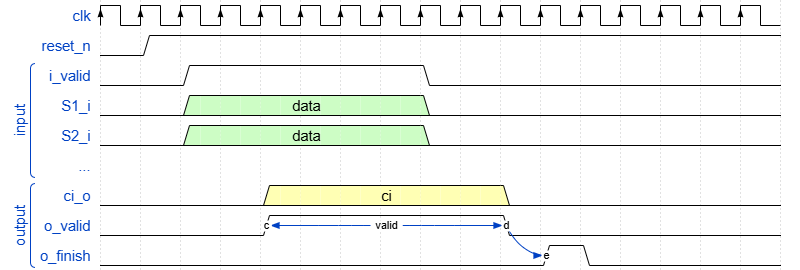
\includegraphics[width=\linewidth]{figures/mrelbpCI.png}
    \caption{Dạng sóng của mô-đun MRELBP\_CI}
    \label{fig:mrelbpCIl}
\end{figure}
\newpage
\subsection{Đặc tả mô-đun NIRD}

Hình \ref{fig:nirdArch} mô tả sơ đồ khối của mô-đun NIRD. Tại mô-đun này ta cần tính hai mô tả là NI và RD theo công thức \ref{eq:relbp_ni} và \ref{eq:relbp_rd}. Vì khi tính RD cần tham chiếu đến hai cửa sổ kích thước khác nhau và dữ liệu của điểm ảnh cũng là đầu ra của bộ lọc trung vị cửa sổ khác nhau, do đó đầu vào sẽ có 2 dữ liệu ứng bán kính r và r1 với r1 = r - 1. Dữ liệu cũng sẽ cần được đệm qua hai bộ đệm có số lượng mô-đun LineBuffer bằng 2*r với r có thể là 2, 4, 6. Sau đó sẽ đi đến mô-đun WindowBuffer với mục đích để hình thành các cửa sổ dữ liệu để thuận lợi cho việc tính toán của các mô-đun sau. Khi tính mô tả NI sẽ là so sánh 8 giá trị trong đường tròn bán kính r so với trung bình tổng bán kính của cửa sổ, do đó sẽ có đầu vào là tổng điểm ảnh của cửa sổ và 8 điểm ảnh trong đường tròn bán kính r. 8 điểm ảnh này sẽ có 4 điểm cần phải suy ra bằng phương pháp nội suy. Với mô tả RD sẽ là so sánh của 8 điểm ảnh đường tròn bán kính r và 8 điểm ảnh trong đường tròn bán kính r1. Dữ liệu sau khi đạt được sẽ cần thực hiện một thao tác gọi là RIU2-mapping hay ánh xạ RIU2. Thực tế, mô-đun này sẽ làm nhiệm vụ chuyển 8-bit có được sau mô-đun NI hoặc RD thành một dạng biểu diễn khác ít bit hơn và mang nhiều ý nghĩa về mặt đặc trưng. Lý thuyết RIU2 đã được trình bày ở tiểu mục \ref{sec:lbp}.

\begin{table}[!ht]
    \centering
    \renewcommand{\arraystretch}{1.3} % Tăng khoảng cách dòng
        \caption{Tham số của mô-đun NIRD}
    \begin{tabular}{|p{3cm} p{4cm} p{8cm}|}
        \hline
        \rowcolor{gray!30}
        \textbf{Tham số } & \textbf{Giá trị mặc định}  & \textbf{Mô tả} \\
        \hline
        COLS & 128 & Kích thước độ rộng của ảnh
        \\ \hline
        ROWS & 128 & Kích thước chiều cao của ảnh
        \\
        \hline
    \end{tabular}

    \label{tab:paramListNIRD}
\end{table}
\begin{table}[!ht]
    \centering
    \renewcommand{\arraystretch}{1.3} % Tăng khoảng cách dòng
        \caption{Danh sách các tín hiệu của mô-đun NIRD}
    \begin{tabular}{|p{3cm} p{2cm} p{2cm} p{8cm}|}
        \hline
        \rowcolor{gray!30}
        \textbf{Tên tín hiệu} & \textbf{Độ rộng} & \textbf{Vào ra} & \textbf{Mô tả} \\
        \hline
        clk & 1 & Vào & Tín hiệu clock \\
        \hline
        rst\_n & 1 & Vào & Reset đồng bộ, kích hoạt mức thấp \\
        \hline 
        data\_r\_i & 8  & Vào &  Dữ liệu vào ứng với bán kính r
        \\ \hline
        i\_r\_valid & 1 & Vào & Tín hiệu thông báo dữ liệu đầu vào bán kính r hợp lệ
        \\ \hline
        data\_r1\_i & 8 & Vào & Dữ liệu vào ứng với bán kính r1
        \\ \hline
        i\_r1\_valid & 1 & Vào & Tín hiệu thông báo dữ liệu vào bán kính r1 hợp lệ
        \\ \hline
        ni\_o & 4 & Ra & Giá trị mô tả NI đầu ra
        \\ \hline
        rd\_o & 4 & Ra & Giá trị mô tả RD đầu ra
        \\ \hline
        o\_valid & 1 & Ra & Tín hiệu thông báo đầu ra là hợp lệ
        \\ \hline
        o\_finish & 1 & Ra & Tín hiệu thông báo kết thúc đầu ra
        \\ \hline
       
    \end{tabular}

    \label{tab:signalListNIRD}
\end{table}

\begin{figure}[!ht]
    \centering
    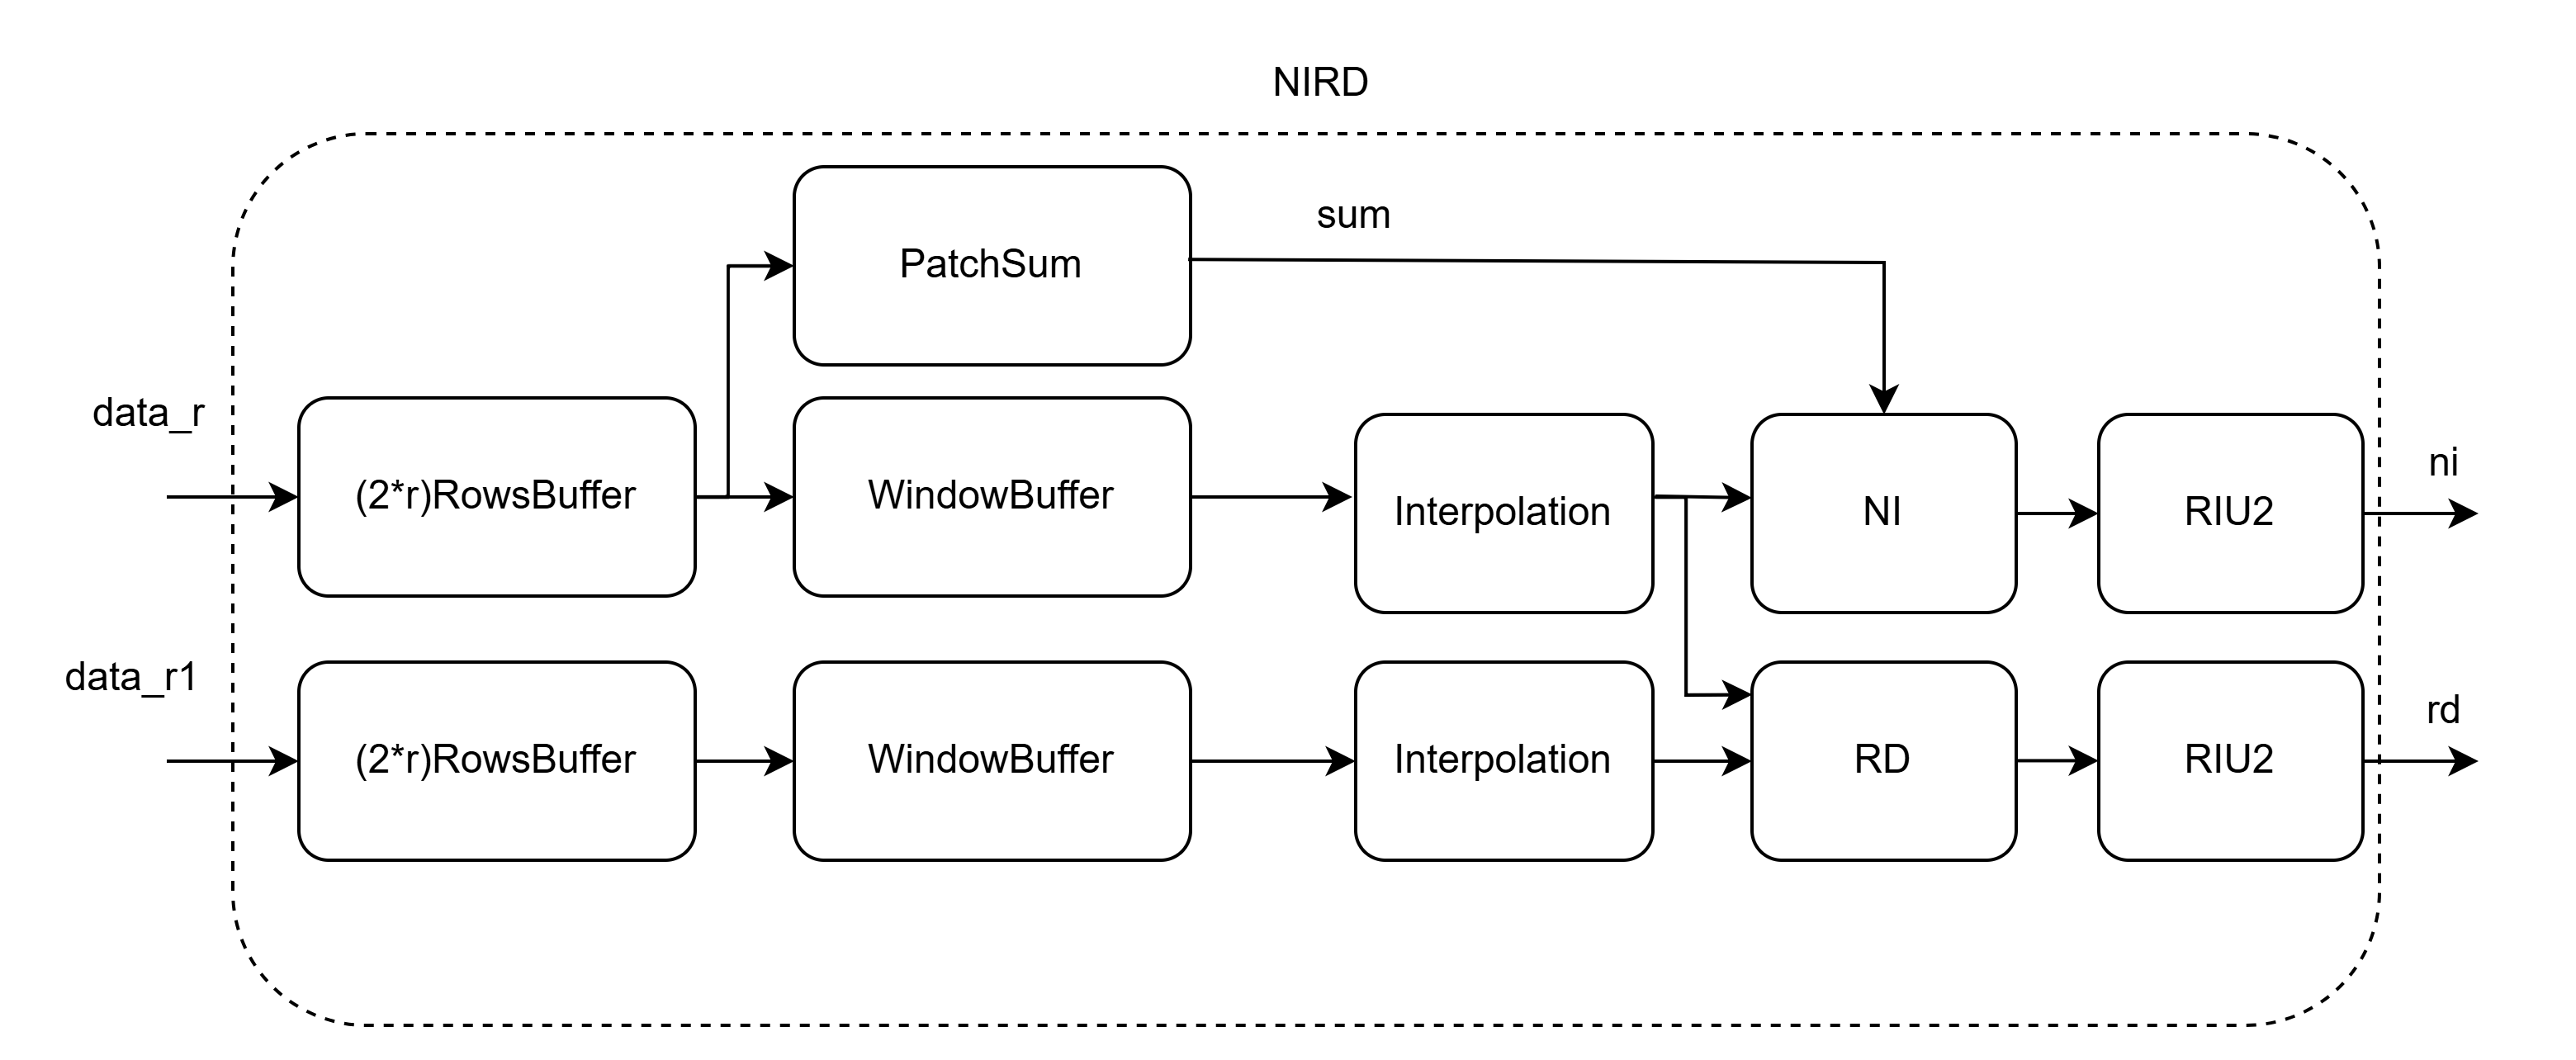
\includegraphics[width=\linewidth]{figures/nirdArch.png}
    \caption{Sơ đồ khối của mô-đun NIRD}
    \label{fig:nirdArch}
\end{figure}
\begin{figure}[!ht]
    \centering
    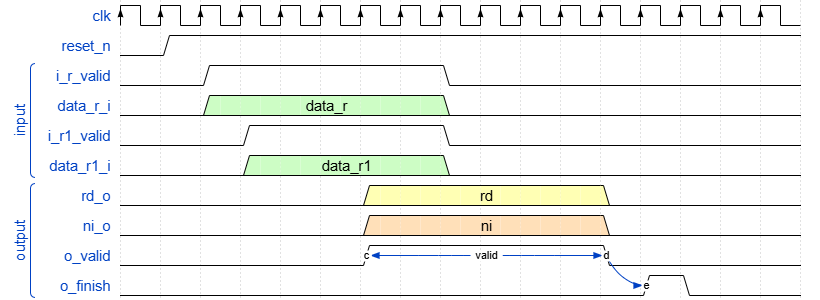
\includegraphics[width=\linewidth]{figures/nird.png}
    \caption{Dạng sóng của mô-đun NIRD}
    \label{fig:nird}
\end{figure}

\subsubsection{Đặc tả mô-đun Interpolation}
mô-đun này sẽ thực hiện chức năng tính toán giá trị chưa biết ở một vài vị trí bán kính bằng phương pháp nội suy. Vì phương pháp này sẽ xuất hiện các giá trị thập phân, để tiện cho việc biểu diễn, sinh viên sử dụng dấu phẩy tĩnh với 8-bit phần nguyên và 16-bit phần thập phân, tổng cộng là 24-bit cho dữ liệu đầu ra. Các dữ liệu ở các góc đặc biệt như 0, 90, 180, 270 độ sẽ không cần thực hiện nội suy, do đó, trong mô-đun cũng sẽ thực thi chức năng đệm dữ liệu để đảm bảo đầu ra có đủ 8 giá trị trên đường tròn bán kính r ở tại một thời điểm. Vì phương pháp nội sử dụng là tuyến tính, do đó cần 4 điểm xung quanh vị trí cần tính, nên ứng với các góc 45, 135, 225 và 315 thì sẽ cần đầy đủ 4 giá trị đầu vào để tính toán.

\begin{table}[!ht]
    \centering
    \renewcommand{\arraystretch}{1.3} % Tăng khoảng cách dòng
        \caption{Tham số của mô-đun Interpolation}
    \begin{tabular}{|p{3cm} p{4cm} p{8cm}|}
        \hline
        \rowcolor{gray!30}
        \textbf{Tham số } & \textbf{Giá trị mặc định}  & \textbf{Mô tả} \\
        \hline
        R & 2 & Kích thước bán kính 
        \\ \hline
        ANGLE & 45 & Giá trị góc
        \\
        \hline
    \end{tabular}

    \label{tab:paramListInterpolation}
\end{table}
\begin{table}[H]
    \centering
    \renewcommand{\arraystretch}{1.2}
        \caption{Danh sách các tín hiệu của mô-đun Interpolation}
    \begin{tabular}{|p{3cm} p{2cm} p{2cm} p{8cm}|}
        \hline
        \rowcolor{gray!30}
        \textbf{Tên tín hiệu} & \textbf{Độ rộng} & \textbf{Vào ra} & \textbf{Mô tả} \\
        \hline
        clk & 1 & Vào & Tín hiệu clock \\
        \hline
        rst\_n & 1 & Vào & Tín hiệu reset đồng bộ, kích hoạt mức thấp \\
        \hline 
        i\_valid & 1 & Vào & Thông báo rằng dữ liệu đầu vào là hợp lệ \\
        \hline
        i\_finish & 1 & Vào & Thông báo không còn dữ liệu đầu vào \\
        \hline
        S\_0\_i & 8 & Vào & Dữ liệu đầu vào tại góc 0 độ \\
        \hline
        S\_90\_i & 8 & Vào & Dữ liệu đầu vào tại góc 90 độ \\
        \hline
        S\_180\_i & 8 & Vào & Dữ liệu đầu vào tại góc 180 độ \\
        \hline
        S\_270\_i & 8 & Vào & Dữ liệu đầu vào tại góc 270 độ \\
        \hline
        S\_45\_i\_1 & 8 & Vào & Dữ liệu đầu vào thứ 1 tại hướng 45 độ \\
        \hline
        S\_45\_i\_2 & 8 & Vào & Dữ liệu đầu vào thứ 2 tại hướng 45 độ \\
        \hline
        S\_45\_i\_3 & 8 & Vào & Dữ liệu đầu vào thứ 3 tại hướng 45 độ \\
        \hline
        S\_45\_i\_4 & 8 & Vào & Dữ liệu đầu vào thứ 4 tại hướng 45 độ \\
        \hline
        S\_135\_i\_1 & 8 & Vào & Dữ liệu đầu vào thứ 1 tại hướng 135 độ \\
        \hline
        S\_135\_i\_2 & 8 & Vào & Dữ liệu đầu vào thứ 2 tại hướng 135 độ \\
        \hline
        S\_135\_i\_3 & 8 & Vào & Dữ liệu đầu vào thứ 3 tại hướng 135 độ \\
        \hline
        S\_135\_i\_4 & 8 & Vào & Dữ liệu đầu vào thứ 4 tại hướng 135 độ \\
        \hline
        S\_225\_i\_1 & 8 & Vào & Dữ liệu đầu vào thứ 1 tại hướng 225 độ \\
        \hline
        S\_225\_i\_2 & 8 & Vào & Dữ liệu đầu vào thứ 2 tại hướng 225 độ \\
        \hline
        S\_225\_i\_3 & 8 & Vào & Dữ liệu đầu vào thứ 3 tại hướng 225 độ \\
        \hline
        S\_225\_i\_4 & 8 & Vào & Dữ liệu đầu vào thứ 4 tại hướng 225 độ \\
        \hline
        S\_315\_i\_1 & 8 & Vào & Dữ liệu đầu vào thứ 1 tại hướng 315 độ \\
        \hline
        S\_315\_i\_2 & 8 & Vào & Dữ liệu đầu vào thứ 2 tại hướng 315 độ \\
        \hline
        S\_315\_i\_3 & 8 & Vào & Dữ liệu đầu vào thứ 3 tại hướng 315 độ \\
        \hline
        S\_315\_i\_4 & 8 & Vào & Dữ liệu đầu vào thứ 4 tại hướng 315 độ \\
        \hline
        S1\_o --> S8\_o & 24 & Ra & Dữ liệu nội suy đầu ra hướng từ 0 -> 315 độ \\
        \hline
        o\_valid & 1 & Ra & Thông báo đầu ra là hợp lệ\\
        \hline
        o\_finish & 1 & Ra & Tín hiệu cho biết đã hết dữ liệu đầu ra \\
        \hline
    \end{tabular}

    \label{tab:signalListInterpolation}
\end{table}












\subsubsection{Đặc tả mô-đun NI}
mô-đun NI sẽ tính toán giá trị của 8 điểm trong đường tròn bán kính r, theo mô tả tại bảng \ref{tab:signalListNI} là từ S1\_r -> S8\_r với giá trị sum\_i. Theo công thức \ref{eq:relbp_ni} thì cần tính trung bình tổng của một cửa sổ, tuy nhiên thực hiện bộ chia sẽ tốn nhiều tài nguyên và phức tạp hơn bộ nhân, do đó mô-đun sẽ triển khai nhân các giá trị đầu vào với tham số \textbf{GAIN}.
\begin{table}[!ht]
    \centering
    \renewcommand{\arraystretch}{1.3} % Tăng khoảng cách dòng
        \caption{Tham số của mô-đun NI}
    \begin{tabular}{|p{3cm} p{4cm} p{8cm}|}
        \hline
        \rowcolor{gray!30}
        \textbf{Tham số } & \textbf{Giá trị mặc định}  & \textbf{Mô tả} \\
        \hline
        WIDTH & 10 & Độ rộng bit của dữ liệu đầu vào sum
        \\ \hline
        GAIN & 25 & Hệ số nhân đối với sum
        \\
        \hline
    \end{tabular}

    \label{tab:paramListNI}
\end{table}
\begin{table}[!ht]
    \centering
    \renewcommand{\arraystretch}{1.3} % Tăng khoảng cách dòng
        \caption{Danh sách các tín hiệu của mô-đun NI}
    \begin{tabular}{|p{3cm} p{2cm} p{2cm} p{8cm}|}
        \hline
        \rowcolor{gray!30}
        \textbf{Tên tín hiệu} & \textbf{Độ rộng} & \textbf{Vào/Ra} & \textbf{Mô tả} \\
        \hline
        clk & 1 & Vào & Tín hiệu clock \\
        \hline
        rst\_n & 1 & Vào & Tín hiệu reset đồng bộ, mức kích hoạt thấp \\
        \hline
        i\_valid & 1 & Vào & Tín hiệu báo dữ liệu đầu vào là hợp lệ \\
        \hline
        i\_finish & 1 & Vào & Tín hiệu báo đã hết dữ liệu đầu vào \\
        \hline
        S1\_r --> S8\_r & 24 & Vào & Các giá trị đầu vào từ 8 hướng tại bán kính r\\
        \hline
        sum\_i & WIDTH & Vào & Tổng giá trị từ mô-đun trước \\
        \hline
        o\_valid & 1 & Ra & Tín hiệu báo dữ liệu đầu ra là hợp lệ\\
        \hline
        o\_finish & 1 & Ra & Tín hiệu báo đã hết dữ liệu đầu ra \\
        \hline
        bit1\_o --> bit8\_o & 1 & Ra & 8 giá trị đầu ra nhị phân ứng với 8 hướng \\
        \hline
    \end{tabular}

    \label{tab:signalListNI}
\end{table}

\begin{figure}[H]
    \centering
    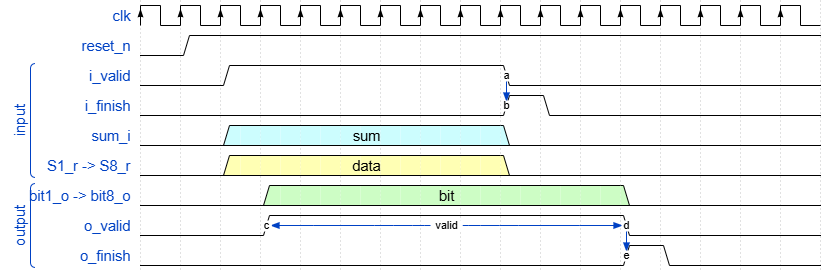
\includegraphics[width=\linewidth]{figures/ni.png}
    \caption{Dạng sóng của mô-đun NI}
    \label{fig:ni}
\end{figure}

\subsubsection{Đặc tả mô-đun RD}
mô-đun RD sẽ tính giá trị mô tả bằng cách so sánh lần lượt các giá trị nằm trên 2 đường tròn bán kính r và r1. Để thuận tiện cho việc đồng bộ dữ liệu, đầu vào sẽ cần có đủ 8 dữ liệu bán kính r và 8 dữ liệu bán kính r1. Dữ liệu đầu ra sẽ lần lượt là 8 bit lần lượt với từng vị trí trên đường tròn. Ví dụ tại vị trí 0 độ, sẽ so sánh giá trị S1\_r và S1\_r1, tương tự với các vị trí khác. 
\begin{table}[H]
    \centering
    \renewcommand{\arraystretch}{1.3} % Tăng khoảng cách dòng
        \caption{Danh sách các tín hiệu của mô-đun RD}
    \begin{tabular}{|p{3cm} p{2cm} p{2cm} p{8cm}|}
        \hline
        \rowcolor{gray!30}
        \textbf{Tên tín hiệu} & \textbf{Độ rộng} & \textbf{Vào/Ra} & \textbf{Mô tả} \\
        \hline
        clk & 1 & Vào & Tín hiệu clock \\
        \hline
        rst\_n & 1 & Vào & Tín hiệu reset đồng bộ, mức kích hoạt thấp \\
        \hline
        i\_valid & 1 & Vào & Tín hiệu báo dữ liệu đầu vào là hợp lệ \\
        \hline
        i\_finish & 1 & Vào & Tín hiệu báo đã hết dữ liệu đầu vào \\
        \hline
        S1\_r --> S8\_r & 24 & Vào & Các giá trị đầu vào từ 8 hướng tại bán kính r\\
        \hline
        S1\_r1 --> S8\_r1 & 24 & Vào & Các giá trị đầu vào từ 8 hướng tại bán kính r1\\
        \hline
        o\_valid & 1 & Ra & Tín hiệu báo dữ liệu đầu ra là hợp lệ\\
        \hline
        o\_finish & 1 & Ra & Tín hiệu báo đã hết dữ liệu đầu ra \\
        \hline
        bit1\_o --> bit8\_o & 1 & Ra & 8 giá trị đầu ra nhị phân ứng với 8 hướng \\
        \hline
    \end{tabular}

    \label{tab:signalListRD}
\end{table}
\begin{figure}[!ht]
    \centering
    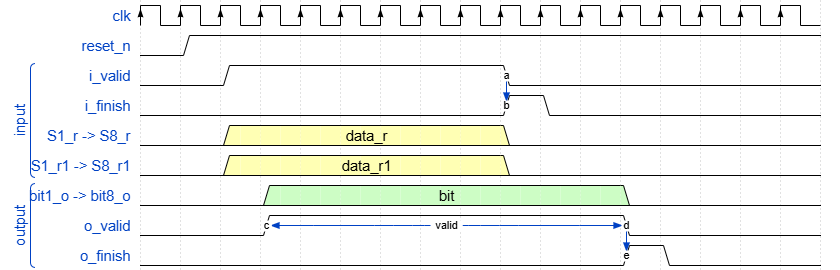
\includegraphics[width=\linewidth]{figures/rd.png}
    \caption{Dạng sóng của mô-đun RD}
    \label{fig:rd}
\end{figure}
\newpage
\subsubsection{Đặc tả mô-đun RIU2}
mô-đun RIU2 sẽ tính toán ra các đặc trưng dựa vào 8-bit đầu vào được tính hoặc từ mô-đun NI hoặc từ mô-đun RD theo công thức \ref{eq:riu2}.
\begin{table}[!ht]
    \centering
    \renewcommand{\arraystretch}{1.3} % Tăng khoảng cách dòng
        \caption{Danh sách các tín hiệu của mô-đun RIU2}
    \begin{tabular}{|p{3cm} p{2cm} p{2cm} p{8cm}|}
        \hline
        \rowcolor{gray!30}
        \textbf{Tên tín hiệu} & \textbf{Độ rộng} & \textbf{Vào/Ra} & \textbf{Mô tả} \\
        \hline
        clk & 1 & Vào & Tín hiệu clock \\
        \hline
        rst\_n & 1 & Vào & Tín hiệu reset đồng bộ, mức kích hoạt thấp \\
        \hline
        i\_valid & 1 & Vào & Tín hiệu báo dữ liệu đầu vào là hợp lệ \\
        \hline
        i\_finish & 1 & Vào & Tín hiệu báo đã hết dữ liệu đầu vào \\
        \hline
        bit1\_i --> bit8\_i & 1 & Vào & 8 giá trị nhị phân đầu vào\\
        \hline
        o\_valid & 1 & Ra & Tín hiệu báo dữ liệu đầu ra là hợp lệ\\
        \hline
        o\_finish & 1 & Ra & Tín hiệu báo đã hết dữ liệu đầu ra \\
        \hline
        data\_o & 4 & Ra & Giá trị riu2 \\
        \hline
    \end{tabular}

    \label{tab:signalListRIU2}
\end{table}
\begin{figure}[!ht]
    \centering
    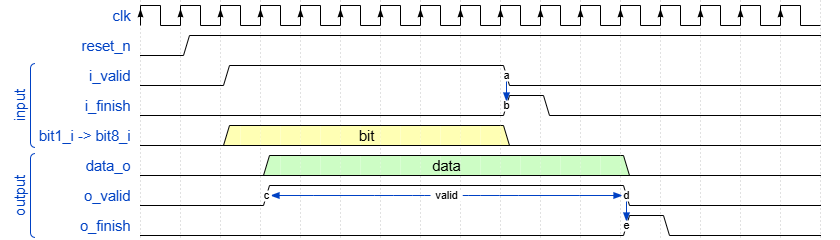
\includegraphics[width=\linewidth]{figures/riu2.png}
    \caption{Dạng sóng của mô-đun RIU2}
    \label{fig:riu2}
\end{figure}
\subsection{Đặc tả mô-đun JointHistogram}

\begin{figure}[H]
    \centering
    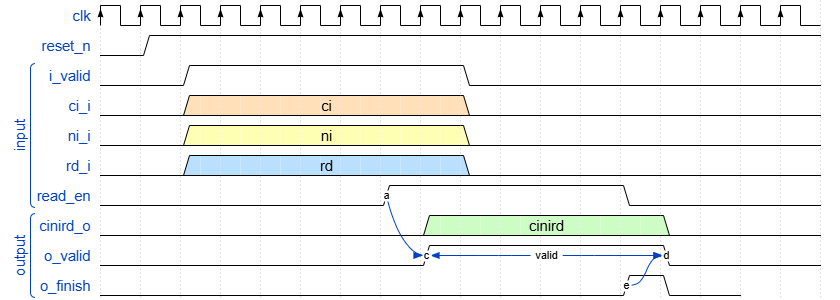
\includegraphics[width=\linewidth]{figures/jointHistogram.png}
    \caption{Biểu đồ sóng của mô-đun JointHistogram}
    \label{fig:jointHistogram}
\end{figure}
mô-đun JointHistogram sẽ có mục đích ghép 3 loại dữ liệu CI, NI và RD theo một công thức toán học nào đó để đạt được đặc trưng đầu ra. Công thức \ref{eq:joint} mô tả cách một đặc trưng được tính toán, mỗi lần đặc trưng này xuất hiện thì giá trị tại bộ nhớ nơi lưu trữ giá trị đấy được tăng lên 1 đơn vị. Vì ci chỉ nhận được giá trị từ 0 -> 1, các giá trị ni và rd sẽ chỉ nhận giá trị từ 0 -> 9 nên thực tế đặc trưng đầu ra có chiều dữ liệu là 200 ứng với mỗi r.
\begin{equation}
    f = ci*100 + ni*10 + rd
    \label{eq:joint}
\end{equation}
\begin{table}[!ht]
    \centering
    \renewcommand{\arraystretch}{1.3} % Tăng khoảng cách dòng
        \caption{Danh sách các tín hiệu của mô-đun JointHistogram}
    \begin{tabular}{|p{3cm} p{2cm} p{2cm} p{8cm}|}
        \hline
        \rowcolor{gray!30}
        \textbf{Tên tín hiệu} & \textbf{Độ rộng} & \textbf{Vào/Ra} & \textbf{Mô tả} \\
        \hline
        clk & 1 & Vào & Tín hiệu clock \\
        \hline
        rst\_n & 1 & Vào & Tín hiệu reset đồng bộ, mức kích hoạt thấp \\
        \hline
        i\_valid & 1 & Vào & Tín hiệu báo dữ liệu đầu vào là hợp lệ \\
        \hline
        ci\_i & 1 & Vào & Mô tả ci đầu vào
        \\ \hline
        ni\_i & 4 & Vào & Mô tả ni đầu vào
        \\ \hline
        rd\_i & 4 & Vào & Mô tả rd đầu vào
        \\ \hline
        read\_en & 1 & Vào & Tín hiệu cho phép đọc từ bộ nhớ
        \\ \hline
        cinird\_o & 16 & Ra & Đặc trưng đầu ra
        \\ \hline
        o\_valid & 1 & Ra & Thông báo dữ liệu đàu ra là hợp lệ
        \\ \hline
        o\_finish & 1 & Ra & Tín hiệu thông báo đã hết dữ liệu đầu ra
        \\
        \hline
    \end{tabular}

    \label{tab:signalListJointHistogram}
\end{table}
\newpage
\clearpage
\phantomsection

\setcounter{chapter}{2}
\chapter[{Thiết kế RTL}]{thiết kế RTL}
Nội dung chương này mô tả về các thiết kế của các mô-đun ở mức Register-Transfer Level (RTL). Mỗi phần mô tả một mô-đun sẽ bao gồm nội dung về kiến trúc RTL và mô tả sơ đồ chuyển trạng thái. Bên cạnh đó, sẽ giải thích nguyên nhân sử dụng kiến trúc đó, ước tính số chu kỳ thực hiện của từng mô-đun. Bố cục của chương sẽ bắt đầu từ các thành phần mô-đun nhỏ đến các mô-đun lớn hơn.

\begin{figure}[!ht]
    \centering
    
\includegraphics[width=1\linewidth]{figures/commonSymbol.png}
    \caption{Định nghĩa các ký hiệu được sử dụng khi mô tả kiến trúc RTL}
    \label{fig:commonSymbol}
\end{figure}
\begin{figure}[!ht]
	\centering
	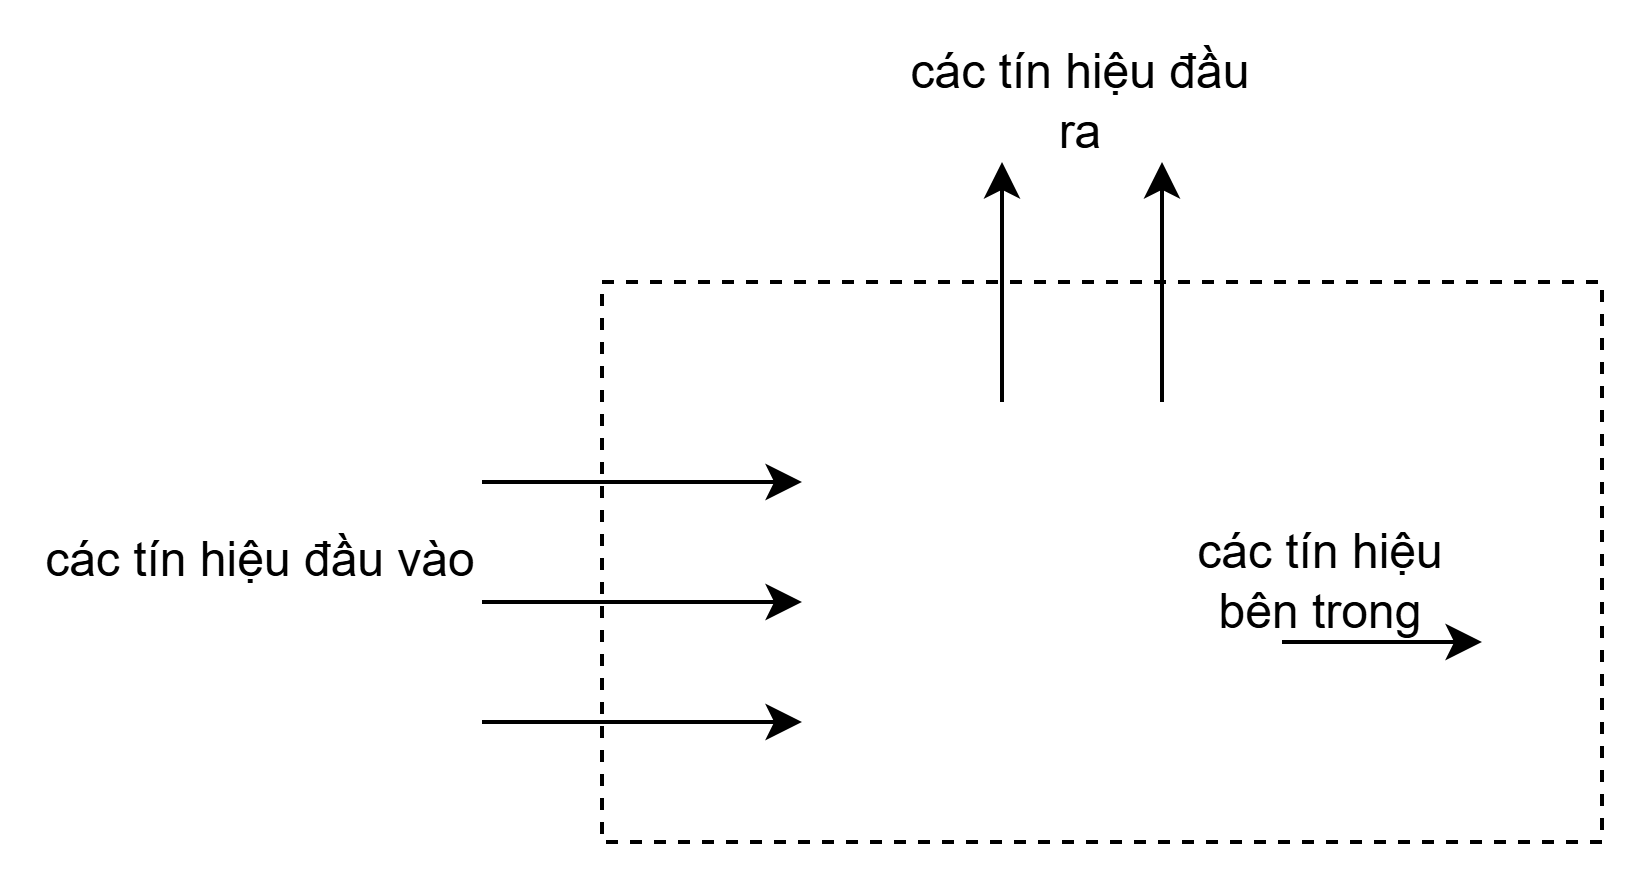
\includegraphics[width=0.7\linewidth]{figures/boxSym.png}
	\caption{Định nghĩa các tín hiệu ra vào một mô-đun}
	\label{fig:boxSym}
\end{figure}
\section{mô-đun MedianProcessing}
\subsection{mô-đun LineBuffer}
Nguyên lý hoạt động của mô-đun LineBuffer là khi có dữ liệu đầu vào, dữ liệu sẽ được ghi vào một vùng nhớ cụ thể, sau khi đạt đến một thời gian hoặc điều kiện đặt ra, dữ liệu từ vùng nhớ đã được ghi sẽ được đọc ra và thứ tự đầu ra sẽ theo nguyên lý FIFO (First In First Out, dữ liệu ghi trước sẽ được đọc ra trước). Hình \ref{fig:lineBuffArchitecture} mô tả kiến trúc RTL của mô-đun LineBuffer và hình \ref{fig:lineBufferTrans} mô tả sơ đồ chuyển trạng thái của bộ \textit{controller} cho mô-đun này. Có thể mô tả ngắn gọn cách thức hoạt động của mô-đun theo mô tả sau: Dữ liệu sẽ được đệm vào bộ nhớ, sau khi dữ liệu ở hàng đầu tiên được đệm (tức là lần đầu tiên bộ nhớ đầy) thì lúc này sẽ có tín hiệu cho phép dữ liệu ra, và quá trình này sẽ kết thúc khi toàn bộ dữ liệu đầu vào được đệm đến đầu ra. 


\textit{Số lượng chu kỳ từ lúc có dữ liệu vào đến khi có dữ liệu đầu ra: } \textbf{DEPTH}


\textit{Số lượng chu kỳ từ lúc có dữ liệu vào đến khi có dữ liệu đầu ra của mô-đun Buffer6Rows: } \textbf{3 * DEPTH}


\begin{figure}[!ht]
    \centering
    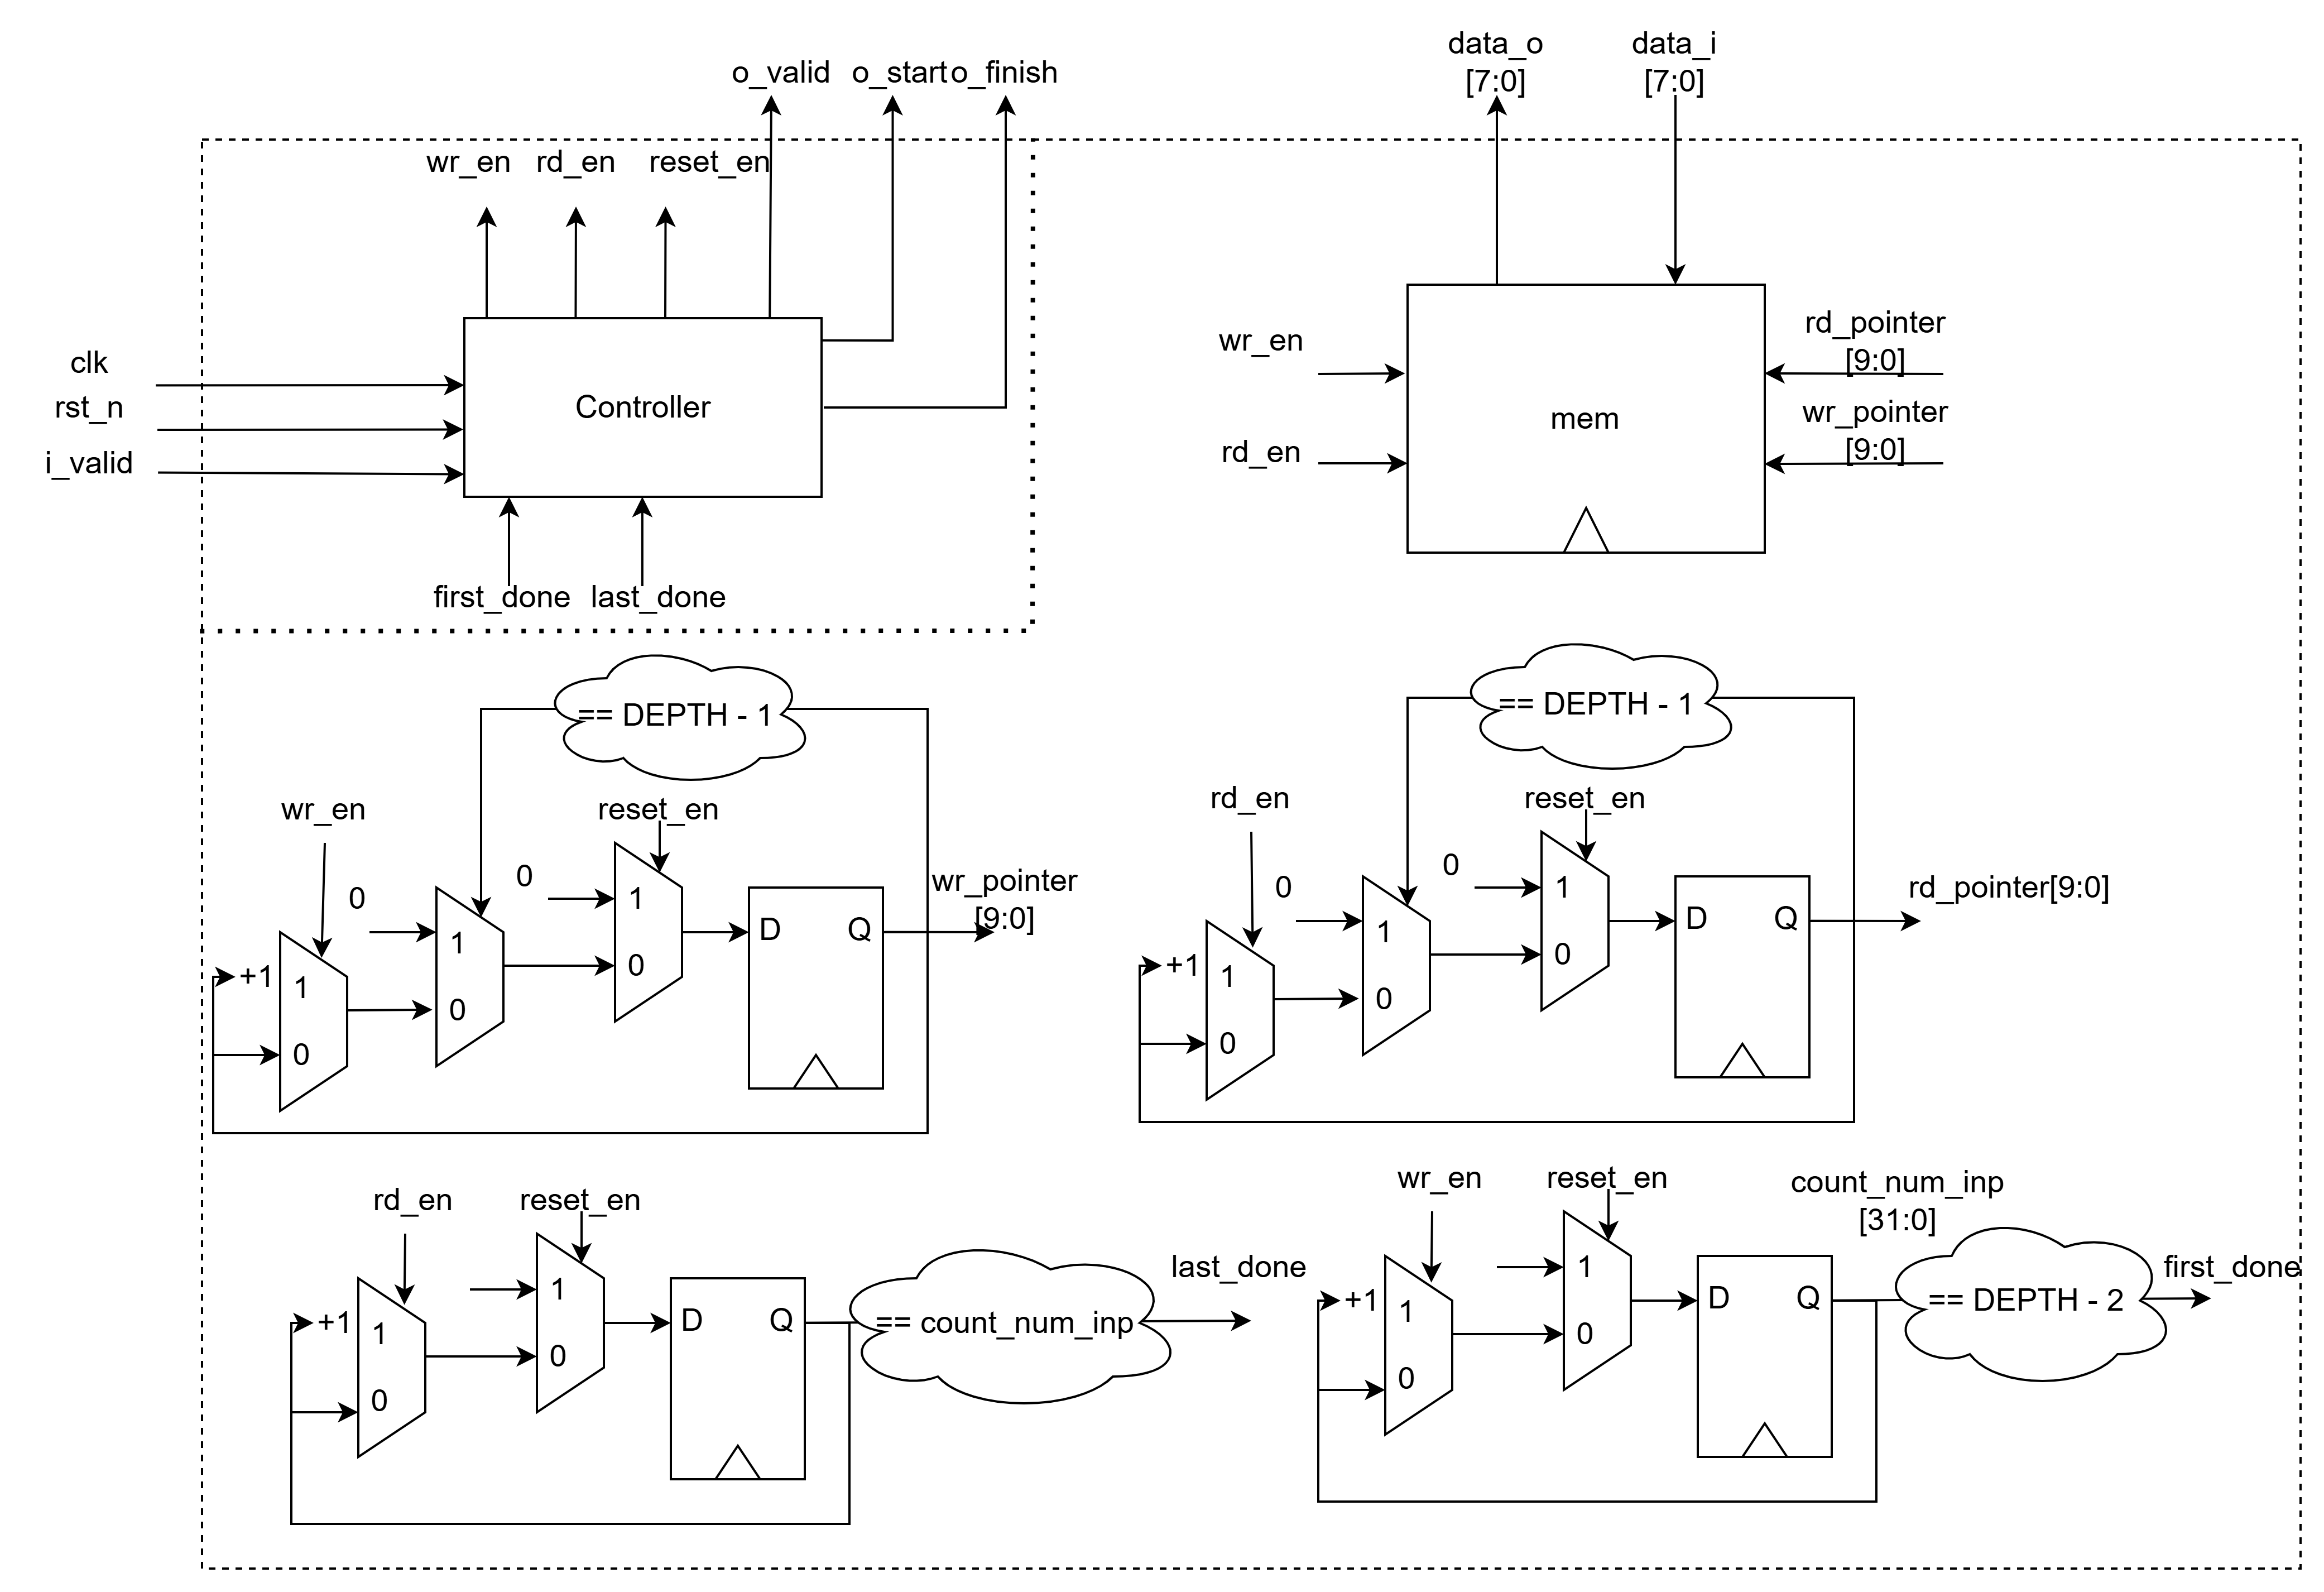
\includegraphics[width=\linewidth]{figures/lineBuffArchitecture.png}
    \caption{Mô tả RTL của mô-đun LineBuffer}
    \label{fig:lineBuffArchitecture}
\end{figure}


\begin{figure}[!ht]
    \centering
    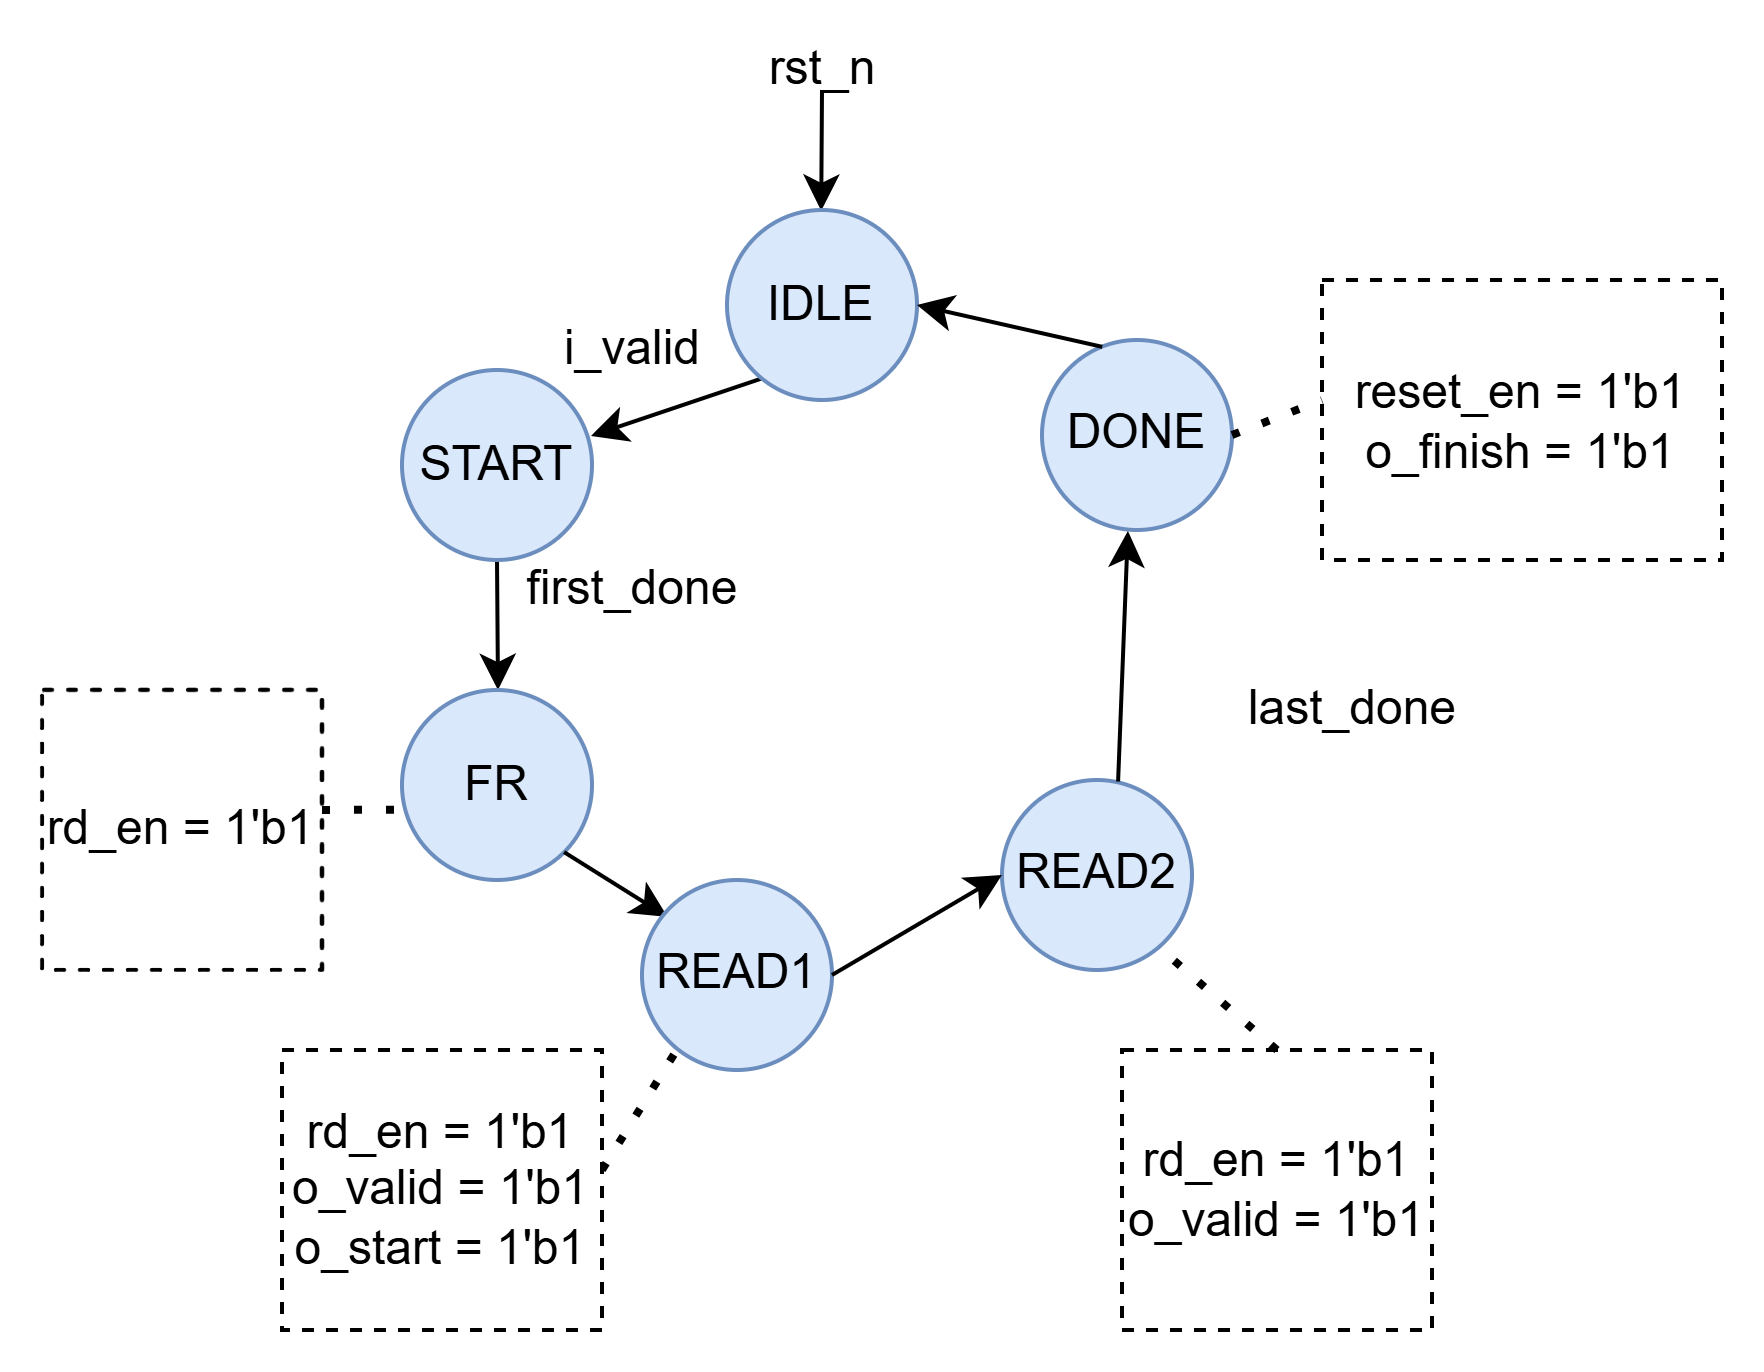
\includegraphics[width=0.8\linewidth]{figures/lineBufferTrans.png}
    \caption{Sơ đồ chuyển trạng thái của mô-đun LineBuffer}
    \label{fig:lineBufferTrans}
\end{figure}


\subsection{mô-đun ZeroPadding}
Mô-đun \textbf{ZeroPadding} sẽ được thiết kế riêng biệt cho ba loại cửa sổ là 3$\times$3, 5$\times$5 và 7$\times$7. Tuy nhiên, chúng đều sử dụng chung một bộ điều khiển, hoạt động theo mô tả ở hình~\ref{fig:zeroPaddingTrans}. Bộ điều khiển này bao gồm bốn trạng thái: \textbf{IDLE}, \textbf{START}, \textbf{DATA} và \textbf{DONE}.

Trạng thái \textbf{START} có chức năng chờ cho đến khi dữ liệu được đệm trong mô-đun ZeroPadding đủ để đáp ứng yêu cầu đầu ra của cửa sổ. Ví dụ, với cửa sổ 3$\times$3, khi xử lý ở rìa ảnh sẽ cần đệm thêm các giá trị 0. Khi đó, trong mô-đun cần có sẵn ít nhất hai điểm ảnh, để sau khi đệm thêm một điểm ảnh 0 sẽ đủ ba điểm ảnh cho một hàng hoặc một cột của cửa sổ.

Trạng thái \textbf{DATA} có chức năng cho phép xuất dữ liệu đầu ra. Khi tín hiệu \textbf{o\_en} ở mức logic 1, các thanh ghi chốt (flip-flop) chứa dữ liệu đầu ra mới được phép truyền dữ liệu ra ngoài. Ví dụ, trong hình~\ref{fig:zero3x3Architecture2}, để dữ liệu đầu ra \textbf{d0\_o} được phép phát ra ngoài, điều kiện là \textit{o\_en} \,\&\, (\textit{i\_row\_lt\_1} \,|\, \textit{i\_col\_lt\_1}). Điều kiện này cũng được áp dụng tương tự cho tất cả các phiên bản khác của mô-đun ZeroPadding.

\begin{figure}[!ht]
    \centering
    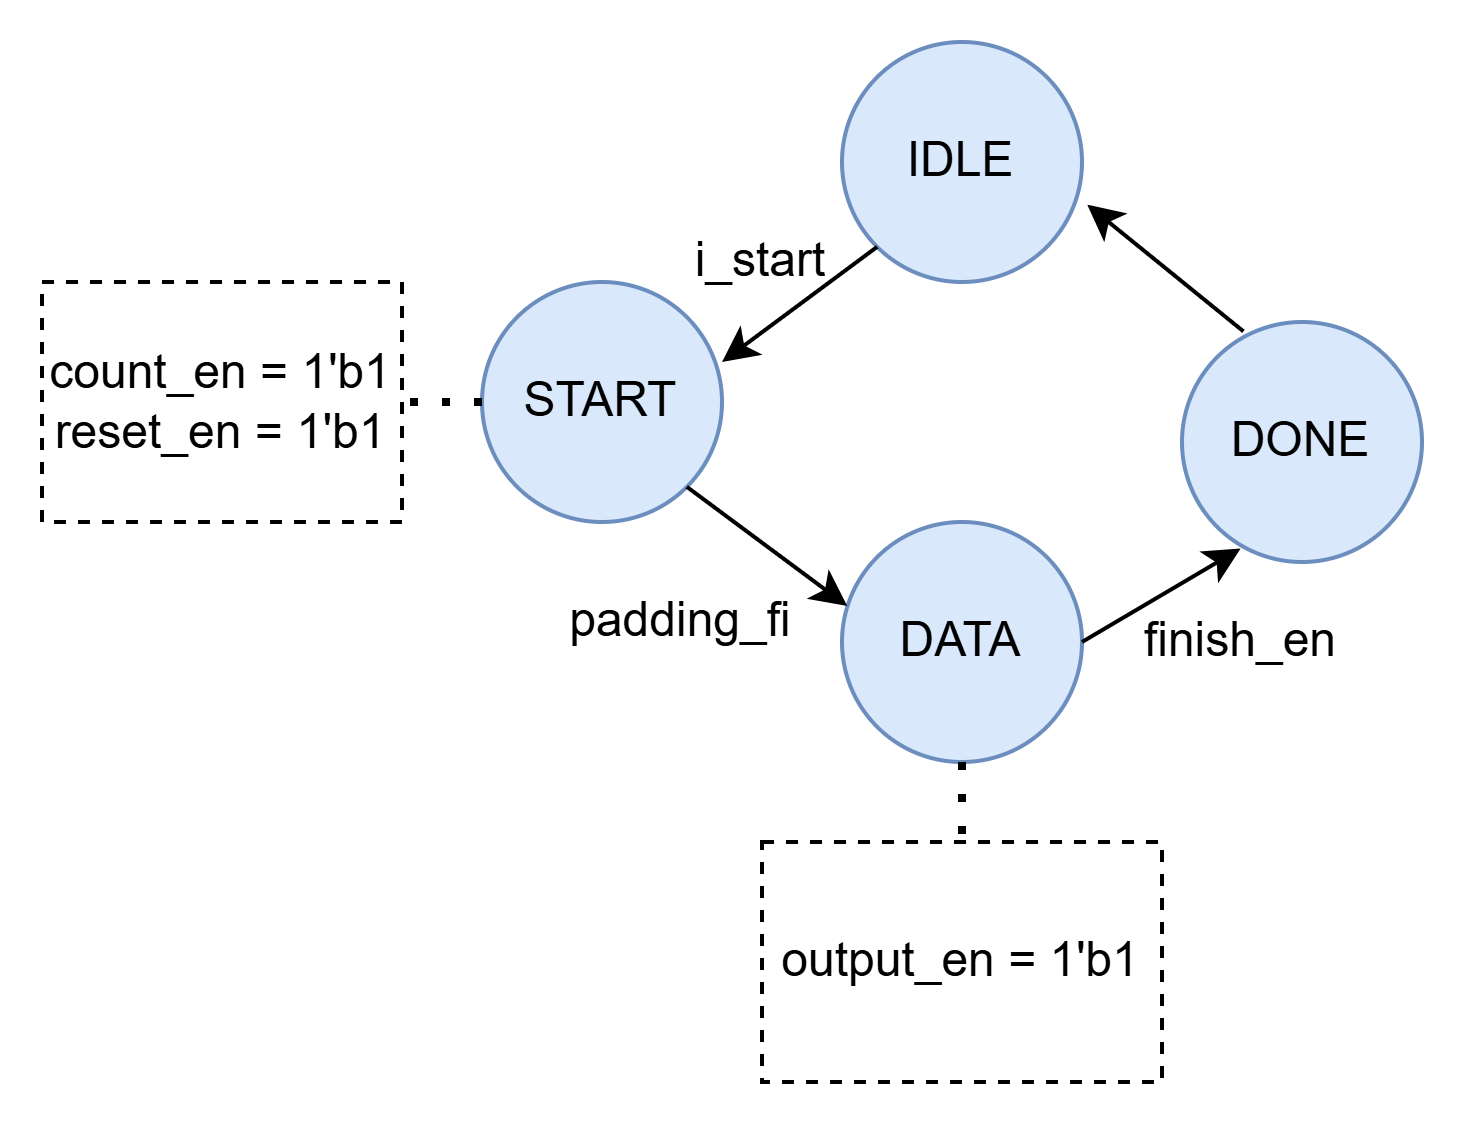
\includegraphics[width=0.6\linewidth]{figures/zeroPaddingTrans.png}
    \caption{Sơ đồ chuyển trạng thái của mô-đun ZeroPadding}
    \label{fig:zeroPaddingTrans}
\end{figure}


\subsubsection{Cửa sổ 3x3}
Hình \ref{fig:zero3x3Architecture1} mô tả kiến trúc RTL đối với bộ ZeroPadding của cửa sổ 3x3, dữ liệu đầu vào của từng hàng sẽ được đệm qua 3 thanh ghi để tạo ra 3 giá trị ứng với mỗi hàng của cửa sổ đầu ra. Dữ liệu đầu ra sẽ dựa vào các điều kiện như ở hình \ref{fig:zero3x3Architecture2}, chính là các tín hiệu điều khiển bộ mạch ghép kênh (mux) để lựa chọn đầu ra là dữ liệu nào.
\begin{figure}[!ht]
    \centering
    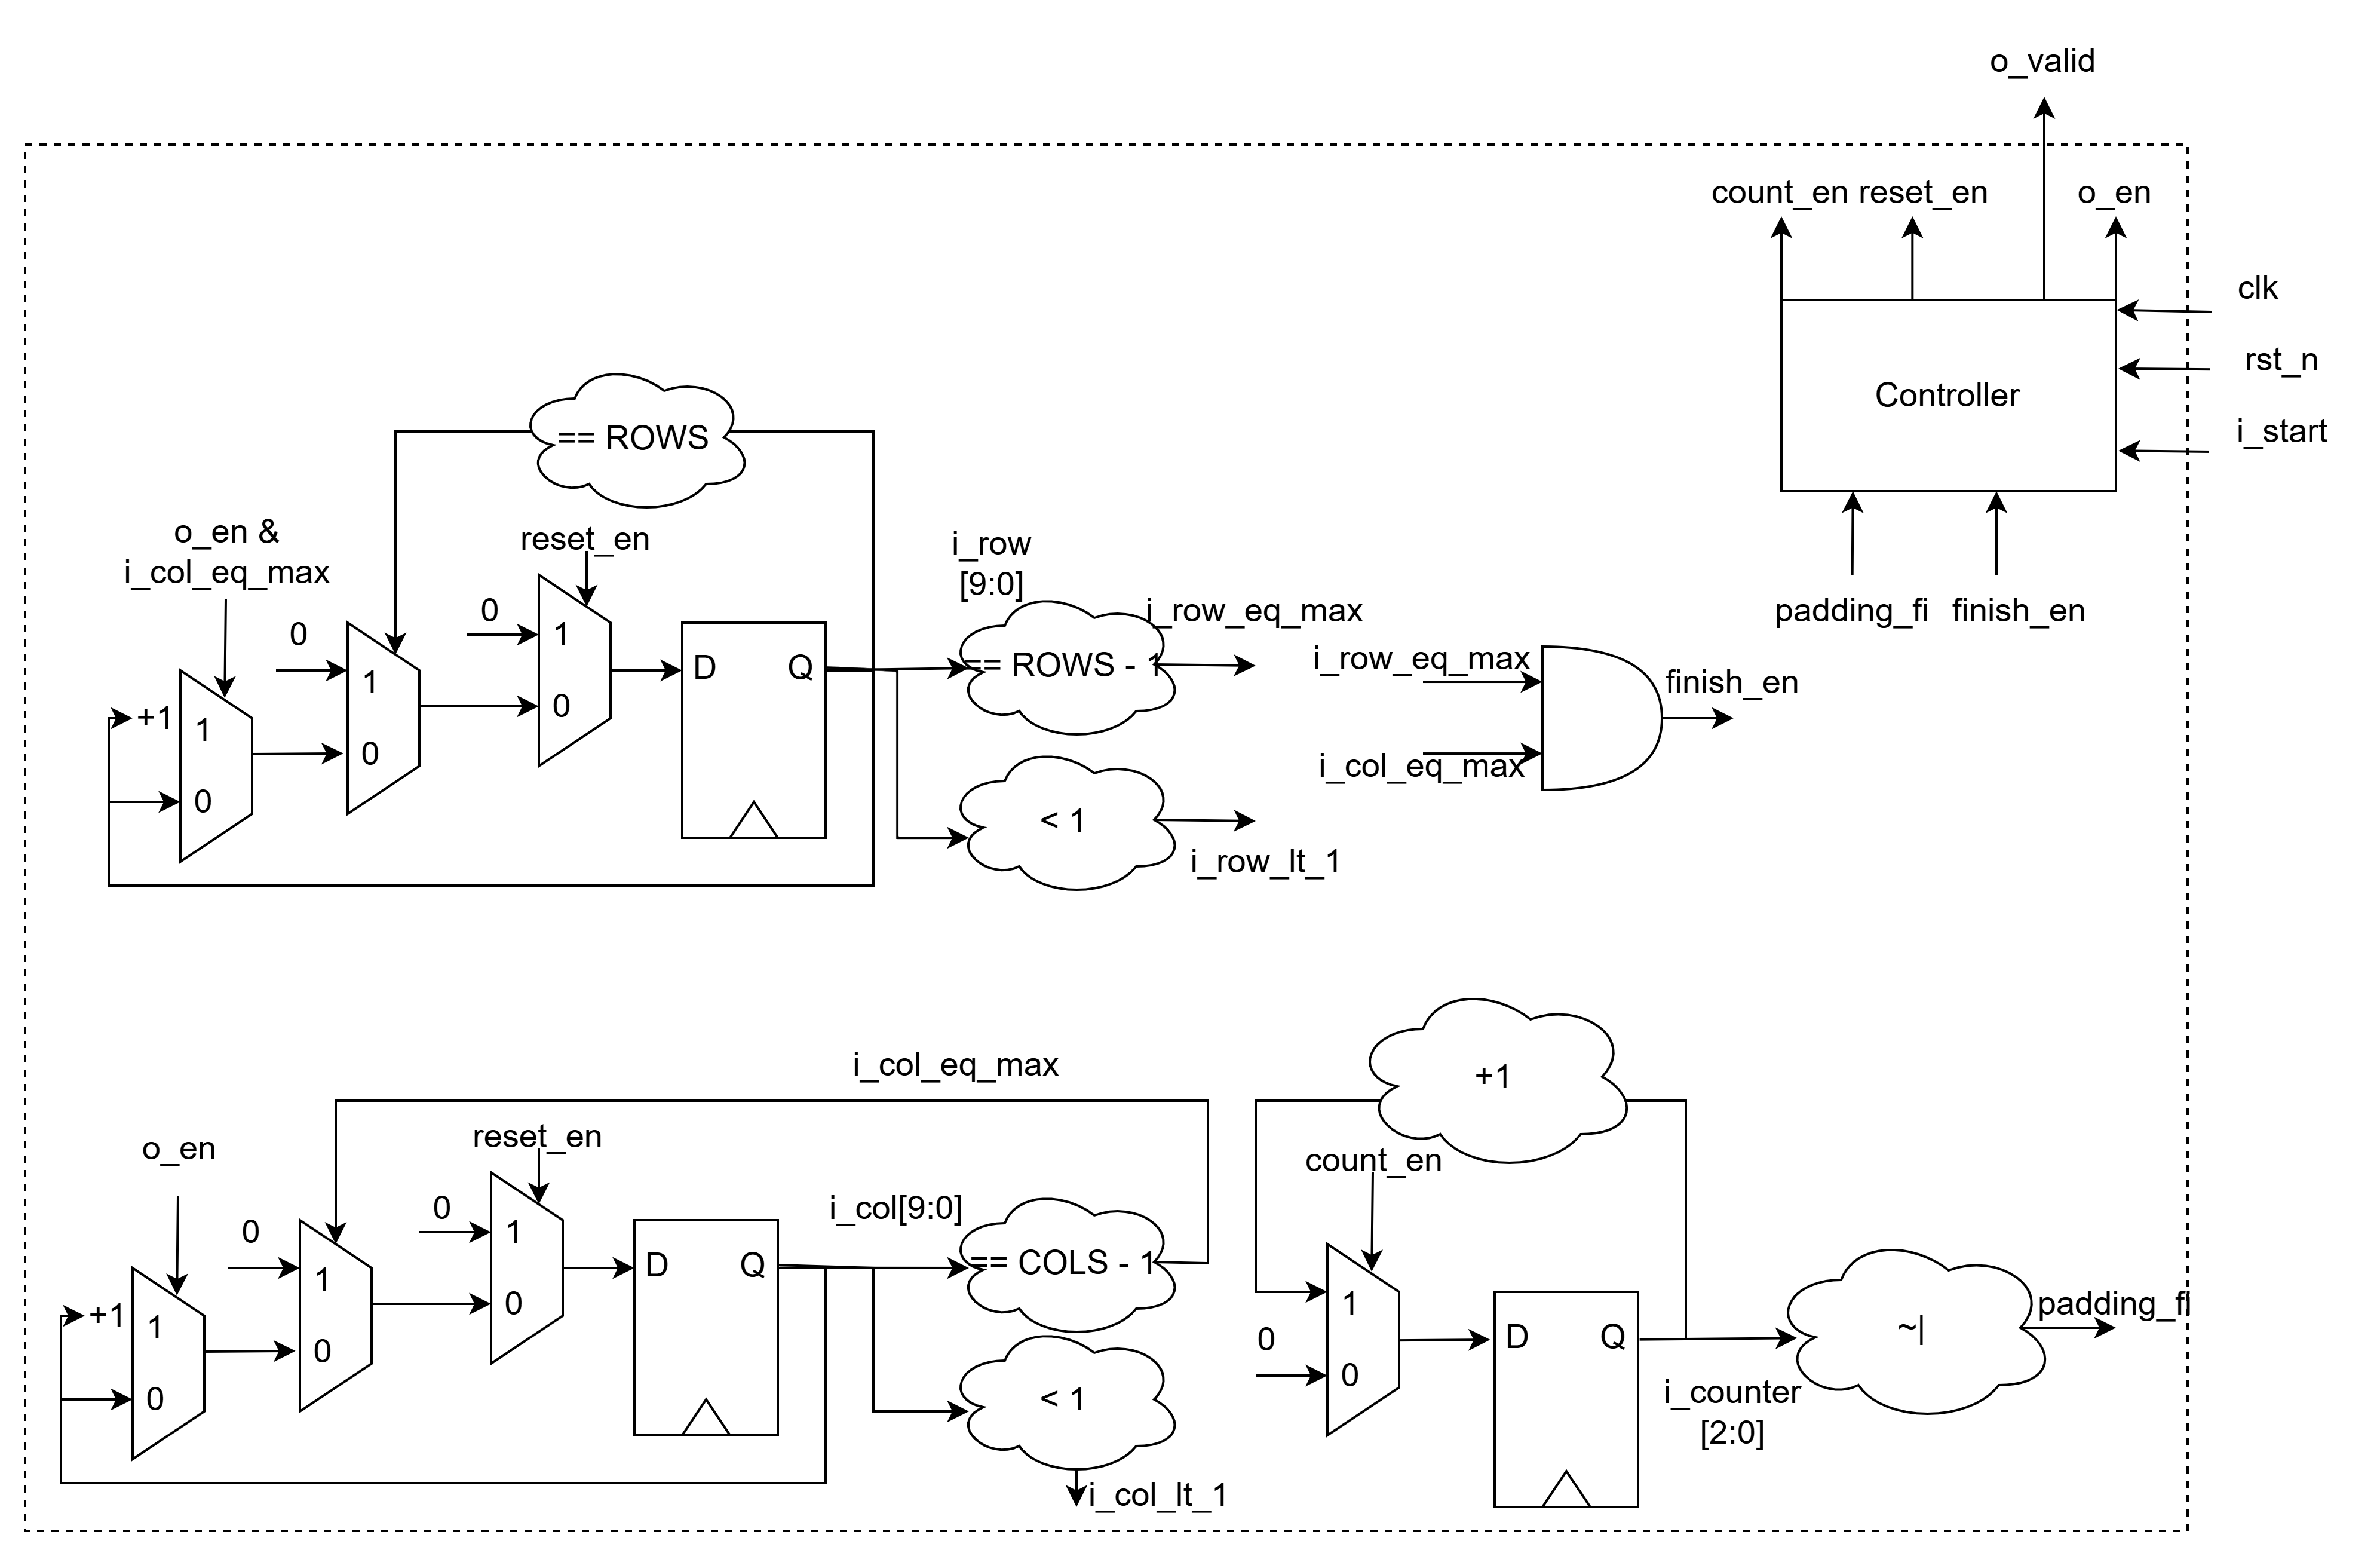
\includegraphics[width=\linewidth]{figures/zero3x3Architecture1.png}
    \caption{Mô tả RTL (1) của mô-đun ZeroPadding ứng với cửa sổ 3x3}
    \label{fig:zero3x3Architecture1}
\end{figure}

\begin{figure}[!ht]
    \centering
    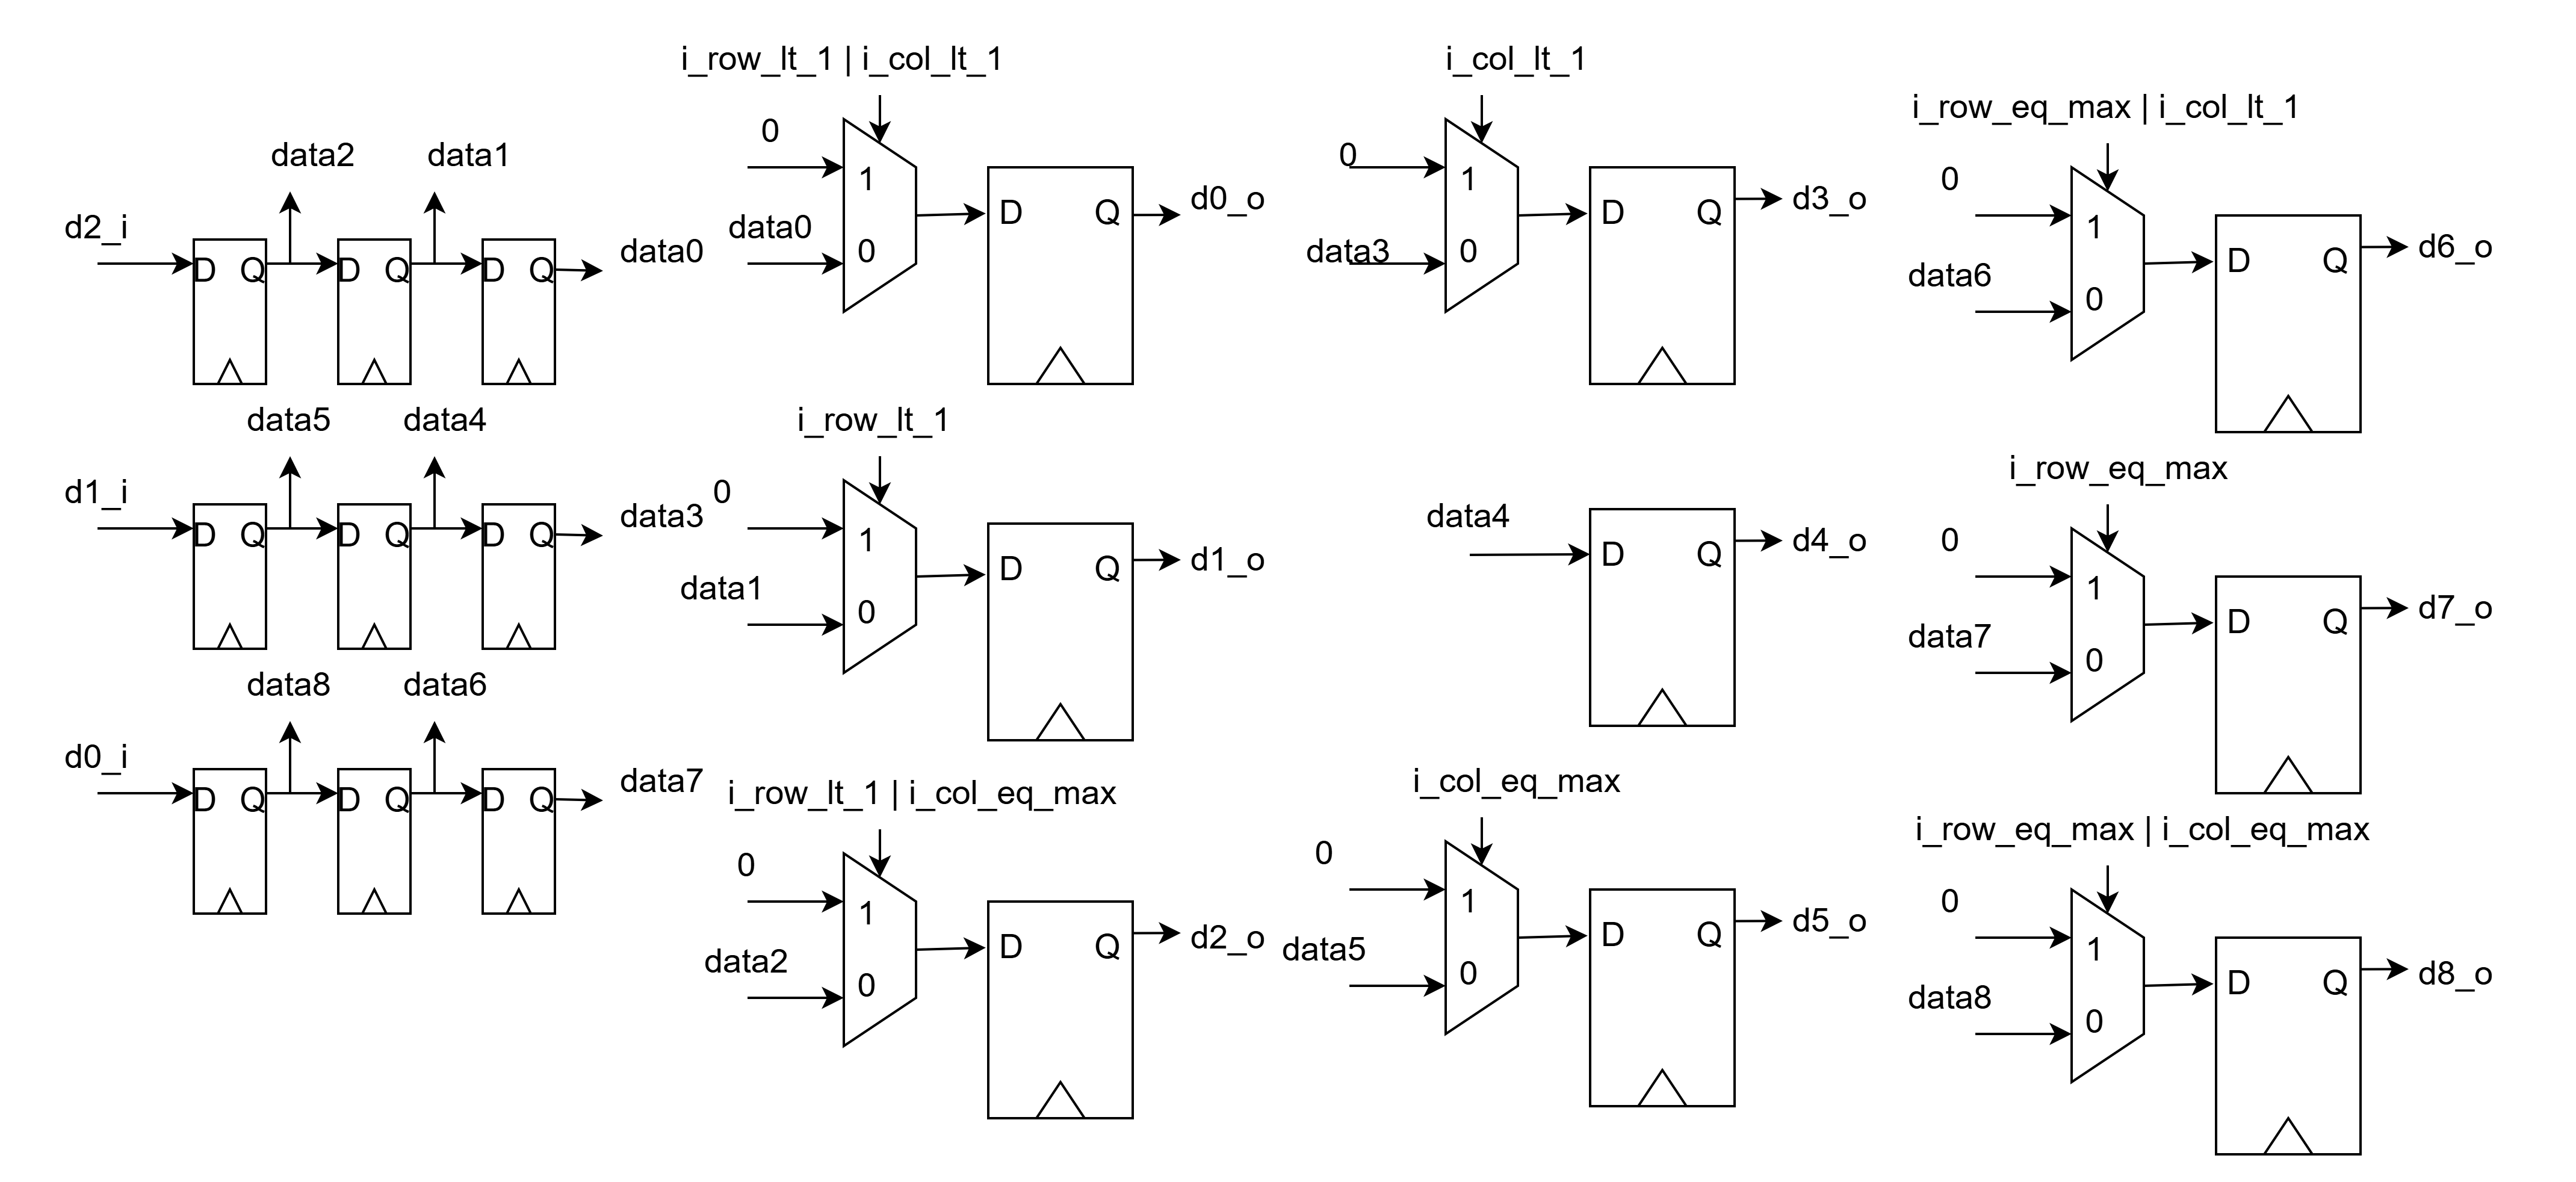
\includegraphics[width=\linewidth]{figures/zero3x3Architecture2.png}
    \caption{Mô tả RTL (2) của mô-đun ZeroPadding ứng với cửa sổ 3x3}
    \label{fig:zero3x3Architecture2}
\end{figure}


\textit{
Bởi vì đối với các cửa sổ 5x5 và 7x7, số lượng các đầu vào và điều kiện cho đầu ra là rất nhiều, khó có thể mô tả bằng hình vẽ, do đó sinh viên sẽ đưa ra bảng giá trị tham chiếu và điều kiện cho từng giá trị đầu ra. }

\subsubsection{Cửa sổ 5x5}
Hình \ref{fig:zero5x5Architecture1} mô tả kiến trúc ở mức RTL cho mô-đun ZeroPadding ứng với cửa sổ đầu vào 5x5. Về cơ bản, nguyên lý hoạt động của mô-đun này tương tự như đối với cửa sổ 3x3, nhưng có thêm một vài điều kiện thêm cho đầu ra như i\_row\_gt\_row\_3, ... Những điều kiện cho đầu ra đã được mô tả chi tiết trong bảng \ref{tab:conditionForOutputZero5x5}. Cột điều kiện tương ứng với tín hiệu chọn cho bộ mạch ghép kênh, khi điều kiện đúng thì đầu ra sẽ là 0, khi điều kiện sai, dữ liệu đầu ra sẽ ứng với giá trị của giá trị tham chiếu đến.
\begin{figure}[!ht]
    \centering
    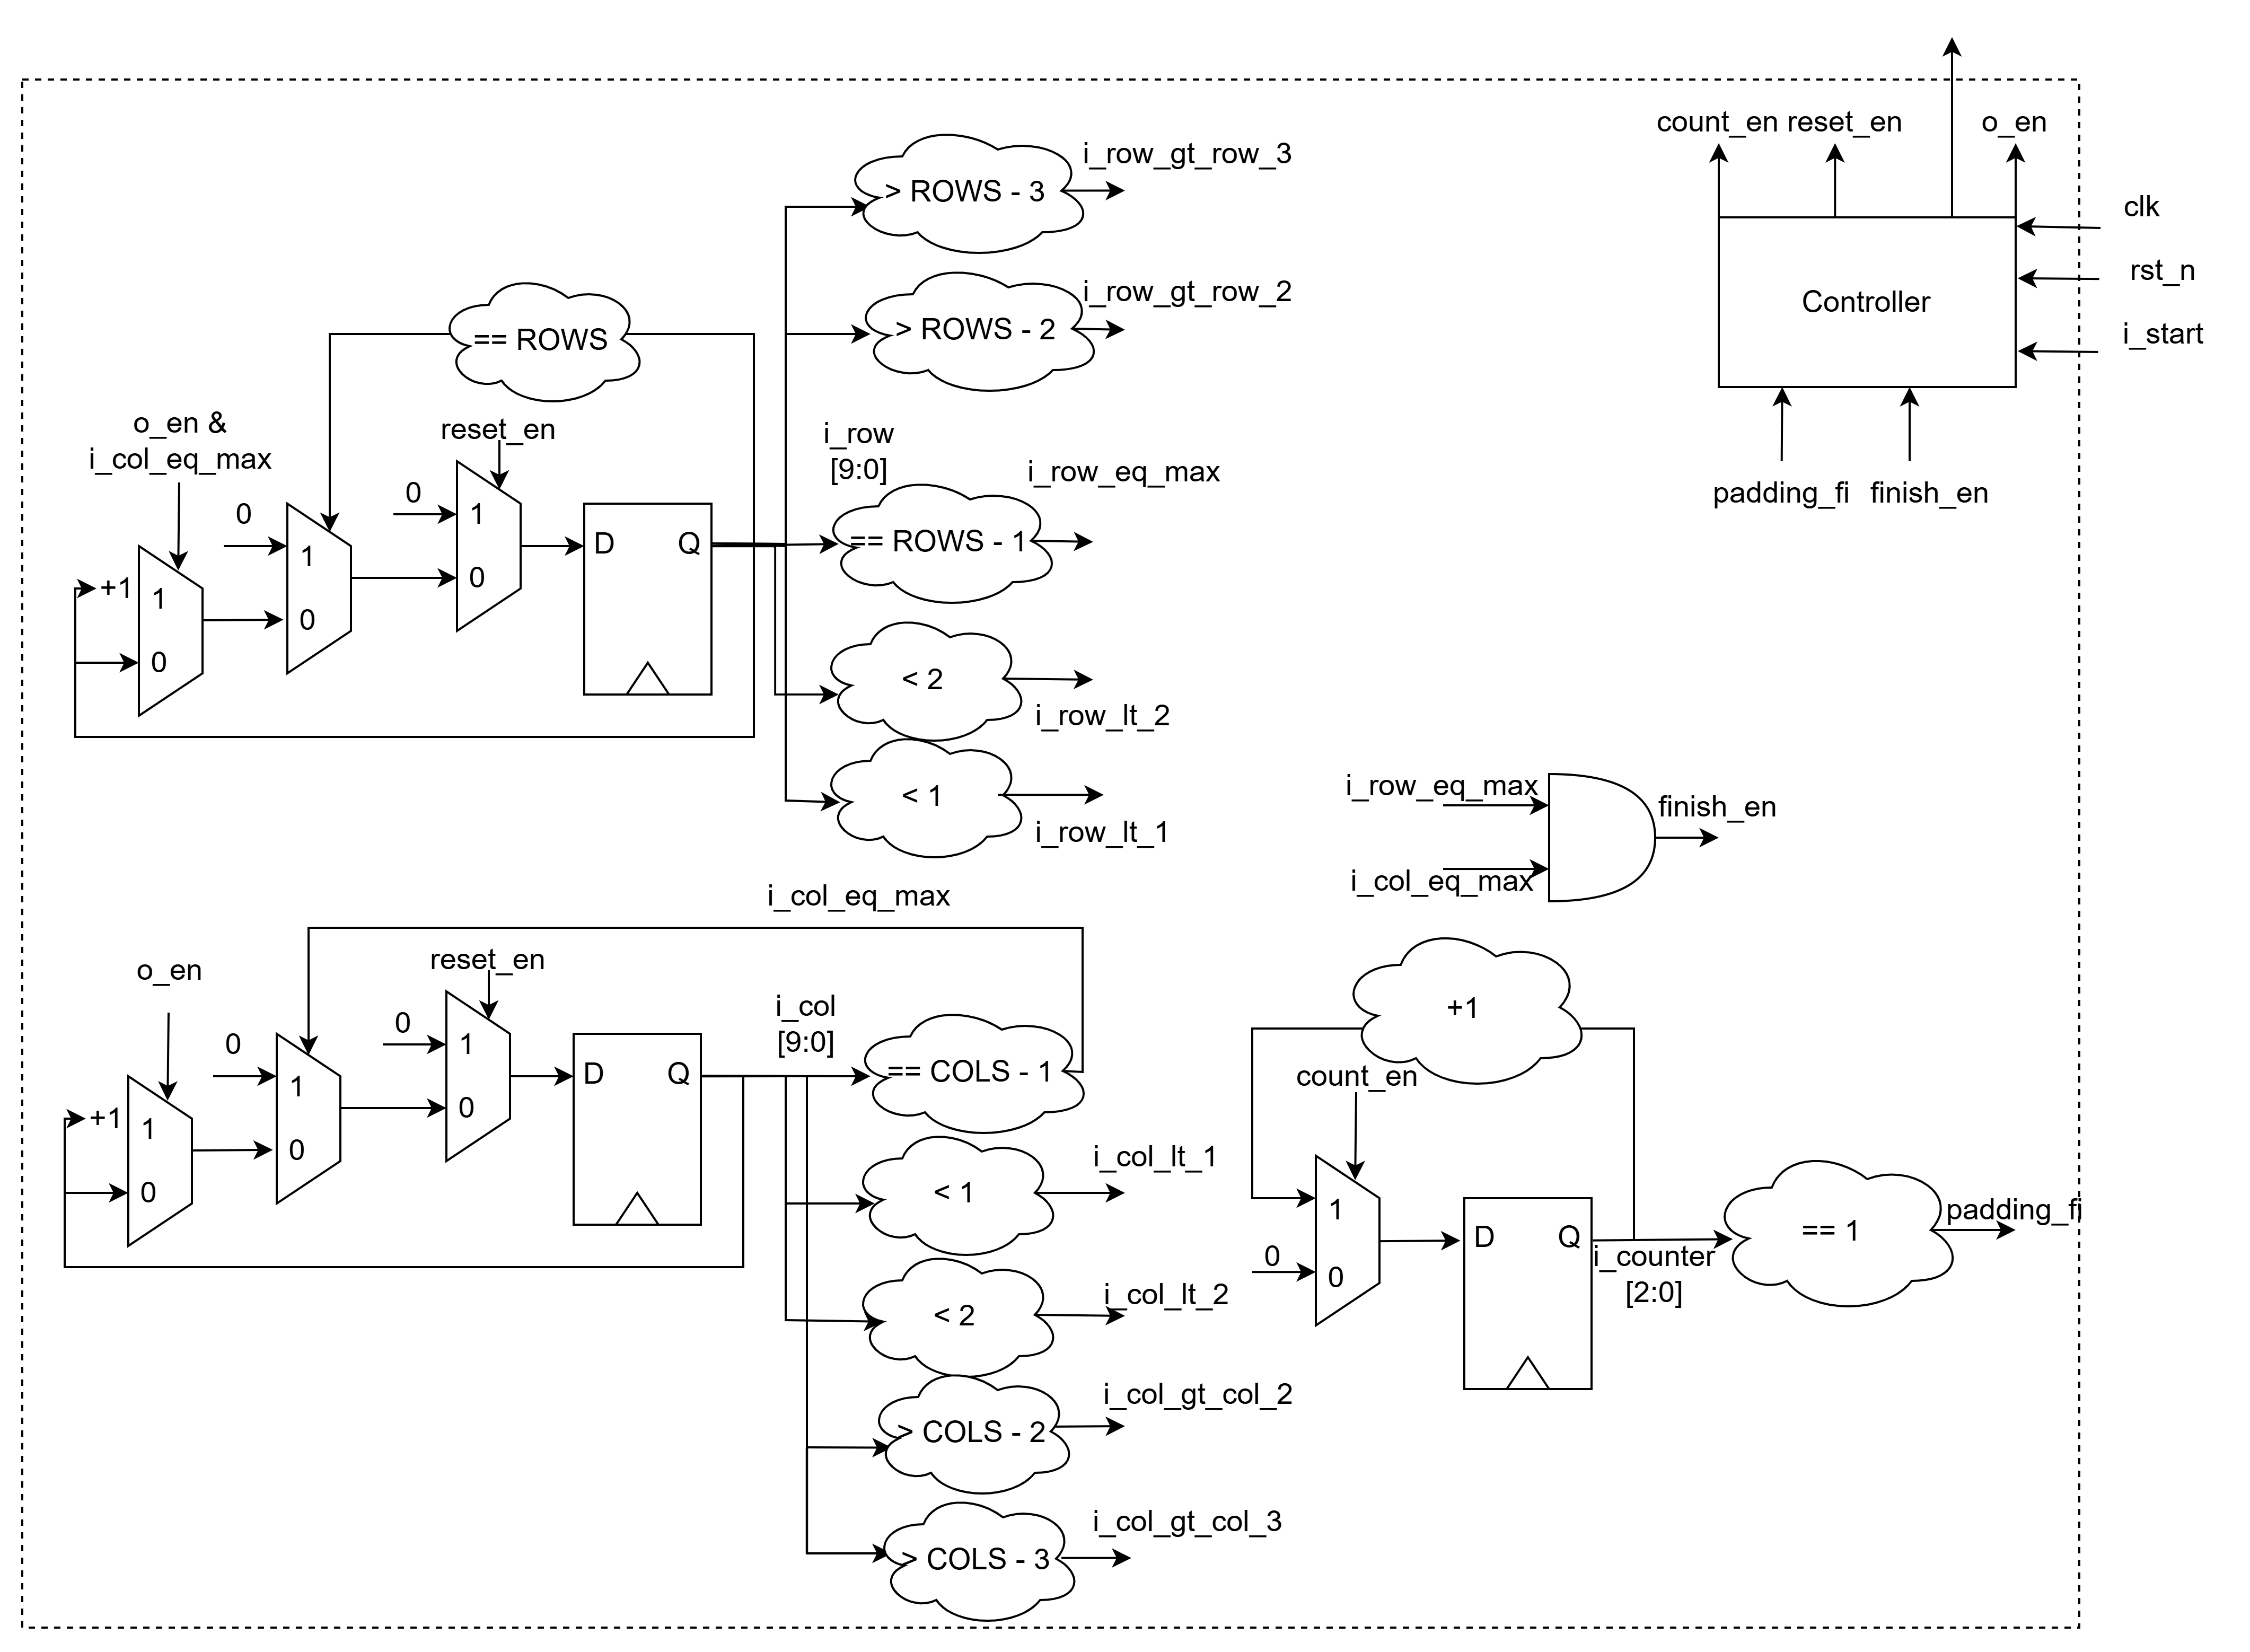
\includegraphics[width=0.9\linewidth]{figures/zero5x5Architecture1.png}
    \caption{Mô tả RTL của mô-đun ZeroPadding ứng với cửa sổ 5x5}
    \label{fig:zero5x5Architecture1}
\end{figure}


\begin{table}[!ht]
    \centering
    \renewcommand{\arraystretch}{1.4}
        \caption{Bảng điều kiện cho dữ liệu đầu ra ứng với cửa sổ 5x5}
    \begin{tabular}{|p{2.2cm} p{7cm} p{4cm}|}
        \hline
        \rowcolor{gray!30}
        \textbf{Tên đầu ra} & \textbf{Điều kiện} & \textbf{Giá trị tham chiếu} \\
        \hline
        d0\_o  & i\_row\_lt\_2 $\vert$ i\_col\_lt\_2         & data0  \\ \hline
        d1\_o  & i\_row\_lt\_2 $\vert$ i\_col\_lt\_1         & data1  \\ \hline
        d2\_o  & i\_row\_lt\_2                                & data2  \\ \hline
        d3\_o  & i\_row\_lt\_2 $\vert$ i\_col\_gt\_col\_2     & data3  \\ \hline
        d4\_o  & i\_row\_lt\_2 $\vert$ i\_col\_gt\_col\_3     & data4  \\ \hline
        d5\_o  & i\_row\_lt\_1 $\vert$ i\_col\_lt\_2         & data5  \\ \hline
        d6\_o  & i\_row\_lt\_1 $\vert$ i\_col\_lt\_1         & data6  \\ \hline
        d7\_o  & i\_row\_lt\_1                                & data7  \\ \hline
        d8\_o  & i\_row\_lt\_1 $\vert$ i\_col\_gt\_col\_2     & data8  \\ \hline
        d9\_o  & i\_row\_lt\_1 $\vert$ i\_col\_gt\_col\_3     & data9  \\ \hline
        d10\_o & i\_col\_lt\_2                                & data10 \\ \hline
        d11\_o & i\_col\_lt\_1                                & data11 \\ \hline
        d12\_o & -- (không có điều kiện)                     & data12 \\ \hline
        d13\_o & i\_col\_gt\_col\_2                           & data13 \\ \hline
        d14\_o & i\_col\_gt\_col\_2                           & data14 \\ \hline
      d15\_o & i\_row\_gt\_row\_2 $\vert$ i\_col\_lt\_2     & data15 \\ \hline
      d16\_o & i\_row\_gt\_row\_2 $\vert$ i\_col\_lt\_1     & data16 \\ \hline
      d17\_o & i\_row\_gt\_row\_2                           & data17 \\ \hline
      d18\_o & i\_row\_gt\_row\_2 $\vert$ i\_col\_gt\_col\_2 & data18 \\ \hline
      d19\_o & i\_row\_gt\_row\_2 $\vert$ i\_col\_gt\_col\_3 & data19 \\ \hline
      d20\_o & i\_row\_gt\_row\_3 $\vert$ i\_col\_lt\_2     & data20 \\ \hline
      d21\_o & i\_row\_gt\_row\_3 $\vert$ i\_col\_lt\_1     & data21 \\ \hline
      d22\_o & i\_row\_gt\_row\_3                           & data22 \\ \hline
      d23\_o & i\_row\_gt\_row\_3 $\vert$ i\_col\_gt\_col\_2 & data23 \\ \hline
      d24\_o & i\_row\_gt\_row\_3 $\vert$ i\_col\_gt\_col\_3 & data24 \\ \hline
    \end{tabular}

    \label{tab:conditionForOutputZero5x5}
\end{table}

\newpage
\subsubsection{Cửa sổ 7x7}
Bảng \ref{tab:numberOfCycleZeroPadding} mô tả số chu kỳ cần thiết từ lúc có dữ liệu vào đến khi có dữ liệu ra của từng mô-đun ZeroPadding ứng với từng loại cửa sổ. Thời gian tính toán tính từ thời điểm mà tín hiệu i\_start chuyển trạng thái đến khi mà tín hiệu đầu ra o\_valid chuyển trạng thái.
\begin{table}[H]
	\centering
	\renewcommand{\arraystretch}{1.3}
		\caption{Số chu kỳ thực hiện của các mô-đun ZeroPadding}
	\begin{tabular}{|p{5cm} p{5cm} |}
		\hline
		\rowcolor{gray!30}
		\textbf{Tên mô-đun} & \textbf{Số chu kỳ}  \\
		\hline
		ZeroPadding3x3  & 3 chu kỳ
		\\ \hline
		ZeroPadding5x5 & 4 chu kỳ
		\\ \hline
		ZeroPadding7x7 & 5 chu kỳ
		\\ \hline
	\end{tabular}

	\label{tab:numberOfCycleZeroPadding}
\end{table}


\begin{figure}[!ht]
    \centering
    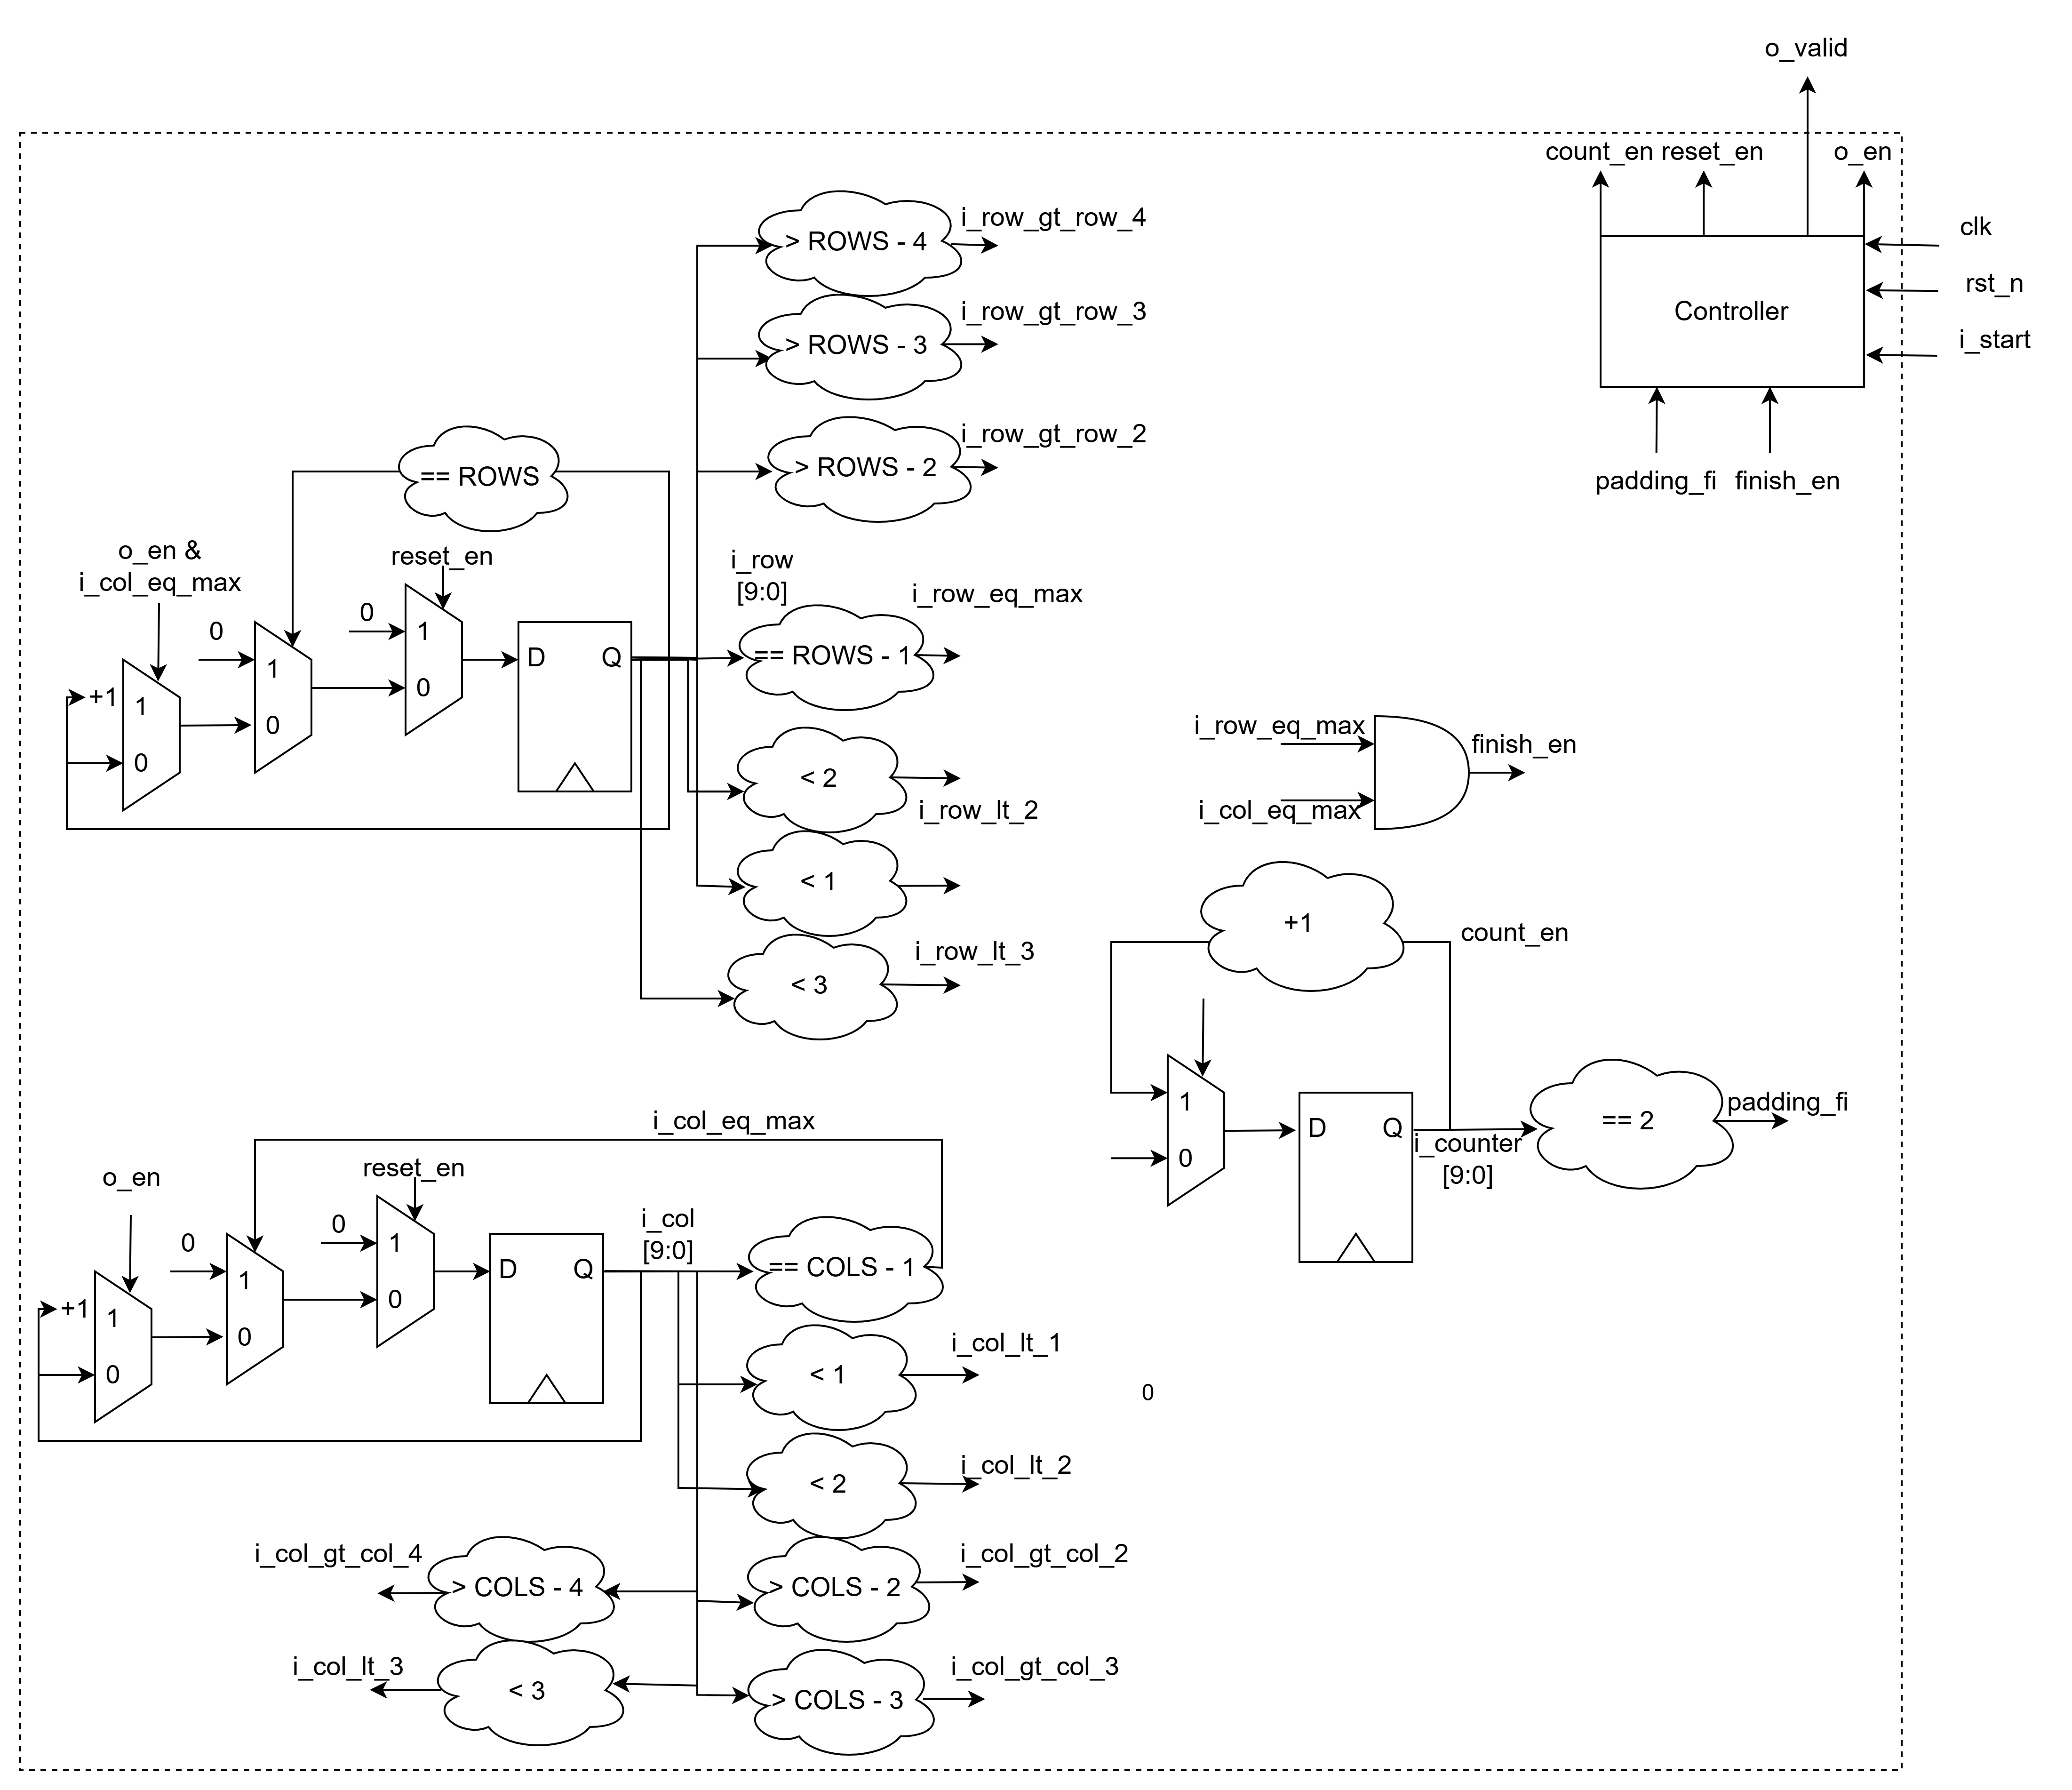
\includegraphics[width=\linewidth]{figures/zero7x7Architecture1.png}
    \caption{Mô tả RTL của mô-đun ZeroPadding ứng với cửa sổ 7x7}
    \label{fig:zero7x7Architecture1}
\end{figure}

\renewcommand{\arraystretch}{1}

\begin{longtable}{|p{3cm}|p{8cm}|p{4cm}|}
			\caption{Bảng điều kiện cho dữ liệu đầu ra ứng với cửa sổ 7x7} \\
	\hline
	\rowcolor{gray!30}
	\textbf{Tên đầu ra} & \textbf{Điều kiện} & \textbf{Giá trị tham chiếu} \\
	\hline
	\endfirsthead
	
	\hline
	\rowcolor{gray!30}
	\textbf{Tên đầu ra} & \textbf{Điều kiện} & \textbf{Giá trị tham chiếu} \\
	\hline
	\endhead
	d0\_o & i\_row\_lt\_3 $\vert$ i\_col\_lt\_3 & data0 \\
	d1\_o & i\_row\_lt\_3 $\vert$ i\_col\_lt\_2 & data1 \\
	d2\_o & i\_row\_lt\_3 $\vert$ i\_col\_lt\_1 & data2 \\
	d3\_o & i\_row\_lt\_3 & data3 \\
	d4\_o & i\_row\_lt\_3 $\vert$ i\_col\_gt\_col\_2 & data4 \\
	d5\_o & i\_row\_lt\_3 $\vert$ i\_col\_gt\_col\_3 & data5 \\
	d6\_o & i\_row\_lt\_3 $\vert$ i\_col\_gt\_col\_4 & data6 \\
	d7\_o & i\_row\_lt\_2 $\vert$ i\_col\_lt\_3 & data7 \\
	d8\_o & i\_row\_lt\_2 $\vert$ i\_col\_lt\_2 & data8 \\
	d9\_o & i\_row\_lt\_2 $\vert$ i\_col\_lt\_1 & data9 \\
	d10\_o & i\_row\_lt\_2 & data10 \\
	d11\_o & i\_row\_lt\_2 $\vert$ i\_col\_gt\_col\_2 & data11 \\
	d12\_o & i\_row\_lt\_2 $\vert$ i\_col\_gt\_col\_3 & data12 \\
	d13\_o & i\_row\_lt\_2 $\vert$ i\_col\_gt\_col\_4 & data13 \\
	d14\_o & i\_row\_lt\_1 $\vert$ i\_col\_lt\_3 & data14 \\
	d15\_o & i\_row\_lt\_1 $\vert$ i\_col\_lt\_2 & data15 \\
	d16\_o & i\_row\_lt\_1 $\vert$ i\_col\_lt\_1 & data16 \\
	d17\_o & i\_row\_lt\_1 & data17 \\
	d18\_o & i\_row\_lt\_1 $\vert$ i\_col\_gt\_col\_2 & data18 \\
	d19\_o & i\_row\_lt\_1 $\vert$ i\_col\_gt\_col\_3 & data19 \\
	d20\_o & i\_row\_lt\_1 $\vert$ i\_col\_gt\_col\_4 & data20 \\
	d21\_o & i\_col\_lt\_3 & data21 \\
	d22\_o & i\_col\_lt\_2 & data22 \\
	d23\_o & i\_col\_lt\_1 & data23 \\
	d24\_o & -- (không có điều kiện) & data24 \\
	d25\_o & i\_col\_gt\_col\_2 & data25 \\
	d26\_o & i\_col\_gt\_col\_3 & data26 \\
	d27\_o & i\_col\_gt\_col\_4 & data27 \\
	d28\_o & i\_row\_gt\_row\_2 $\vert$ i\_col\_lt\_3 & data28 \\
	d29\_o & i\_row\_gt\_row\_2 $\vert$ i\_col\_lt\_2 & data29 \\
	d30\_o & i\_row\_gt\_row\_2 $\vert$ i\_col\_lt\_1 & data30 \\
	d31\_o & i\_row\_gt\_row\_2 & data31 \\
	d32\_o & i\_row\_gt\_row\_2 $\vert$ i\_col\_gt\_col\_2 & data32 \\
	d33\_o & i\_row\_gt\_row\_2 $\vert$ i\_col\_gt\_col\_3 & data33 \\
	d34\_o & i\_row\_gt\_row\_2 $\vert$ i\_col\_gt\_col\_4 & data34 \\
	d35\_o & i\_row\_gt\_row\_3 $\vert$ i\_col\_lt\_3 & data35 \\
	d36\_o & i\_row\_gt\_row\_3 $\vert$ i\_col\_lt\_2 & data36 \\
	d37\_o & i\_row\_gt\_row\_3 $\vert$ i\_col\_lt\_1 & data37 \\
	d38\_o & i\_row\_gt\_row\_3 & data38 \\
	d39\_o & i\_row\_gt\_row\_3 $\vert$ i\_col\_gt\_col\_2 & data39 \\
	d40\_o & i\_row\_gt\_row\_3 $\vert$ i\_col\_gt\_col\_3 & data40 \\
	d41\_o & i\_row\_gt\_row\_3 $\vert$ i\_col\_gt\_col\_4 & data41 \\
	d42\_o & i\_row\_gt\_row\_4 $\vert$ i\_col\_lt\_3 & data42 \\
	d43\_o & i\_row\_gt\_row\_4 $\vert$ i\_col\_lt\_2 & data43 \\
	d44\_o & i\_row\_gt\_row\_4 $\vert$ i\_col\_lt\_1 & data44 \\
	d45\_o & i\_row\_gt\_row\_4 & data45 \\
	d46\_o & i\_row\_gt\_row\_4 $\vert$ i\_col\_gt\_col\_2 & data46 \\
	d47\_o & i\_row\_gt\_row\_4 $\vert$ i\_col\_gt\_col\_3 & data47 \\
	d48\_o & i\_row\_gt\_row\_4 $\vert$ i\_col\_gt\_col\_4 & data48 \\
	\hline

		\label{tab:conditionForOutputZero7x7}
\end{longtable}

\subsection{mô-đun MedianCalculation}
mô-đun MedianCalculation sẽ tính toán giá trị trung vị đầu ra dựa trên các điểm ảnh đầu vào. Vì sẽ tính toán cho riêng biệt 3 cửa sổ là 3x3, 5x5 và 7x7, nên để tối ưu, sinh viên sẽ thiết kế riêng 3 bộ tính trung vị ứng với từng cửa sổ.


\subsubsection{Thuật toán tính toán trung vị}
Đầu tiên, một mạng sắp xếp(sorting network) được định nghĩa là một chuỗi các hoạt động so sánh và hoán đổi các phần tử. Mặc dù một mạng sắp xếp với một số lượng phân tử cố định cần yêu cầu nhiều phép so sánh hơn so với các phương pháp so sánh như sắp xếp nhanh, ... Tuy nhiên, nó có một lợi thế là không phải phụ thuộc vào kết quả của những phép so sánh trước đó, do đó không cần sự điều khiển. Từ đó, nó sẽ phù hợp với các bài toán tính toán song song.


Hình \ref{fig:sortingEx3} mô tả một mạng sắp xếp cho 3 phần tử với out0, out1 và out2 lần lượt là các giá trị nhỏ nhất, trung vị và lớn nhất trong 3 phần tử đó. Các ô 1, 2 và 3 là các bộ so sánh và hoán đổi có kiến trúc được mô tả ở hình \ref{fig:node}. \textit{\textbf{Chú ý}: Ở trong các hình ảnh bên dưới, mạng sắp xếp sẽ được gọi là \textbf{Sorting\_network} và bộ so sánh và hoán đổi được gọi là \textbf{Node}}. Thuật toán \ref{alg:medianFilterAlgo} mô tả cách tính toán giá trị trung vị ứng với một mảng có kích thước NxN, bao gồm 3 bước chính là sắp xếp từng hàng, sắp xếp từng cột, và sau đó sắp xếp các đường chéo với điều kiện xác định. Thuật toán này rất phù hợp với các bộ có kích thước nhỏ, và thành phần phù hợp để triển khai là các mạng sắp xếp.

\begin{algorithm}
	\caption{Tìm trung vị của một mảng NxN với N là số lẻ \cite{altivec}}
	\begin{algorithmic}[1]
		\State \textbf{Đầu vào:} Một mảng $A$ có kích thước $N \times N$
		\State \textbf{Đầu ra:} Giá trị trung vị của mảng
		\State $M = \frac{N - 1}{2}$
		\State Sắp xếp các hàng của mảng theo thứ tự tăng dần
		\State Sắp xếp các cột của mảng theo thứ tự tăng dần
		\State Sắp xếp các đường chéo có độ dốc $k$
		\For{$k = 1$ to $M$}
		\For{$s = k \cdot (M+1)$ to $k \cdot (M-1) + (N-1)$}
		\State Dòng được sắp xếp được xác định bởi phương trình $k \cdot r + c = s$
		\State Với mọi $r$: $A[r-1, s - k \cdot (r-1)] \leq A[r, s - k \cdot r]$
		\EndFor
		\EndFor
		\State \textbf{Trả về:} $A[M, M]$
	\end{algorithmic}
	\label{alg:medianFilterAlgo}
\end{algorithm}




\begin{figure}[!ht]
	\centering
	\begin{minipage}[b]{0.48\linewidth}
		\centering
		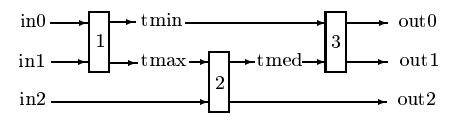
\includegraphics[width=\linewidth]{figures/sortingEx3.png}
		\caption{Mô tả về mạng sắp xếp với 3 phần tử \cite{altivec}}
		\label{fig:sortingEx3}
	\end{minipage}
	\hfill
	\begin{minipage}[b]{0.48\linewidth}
		\centering
		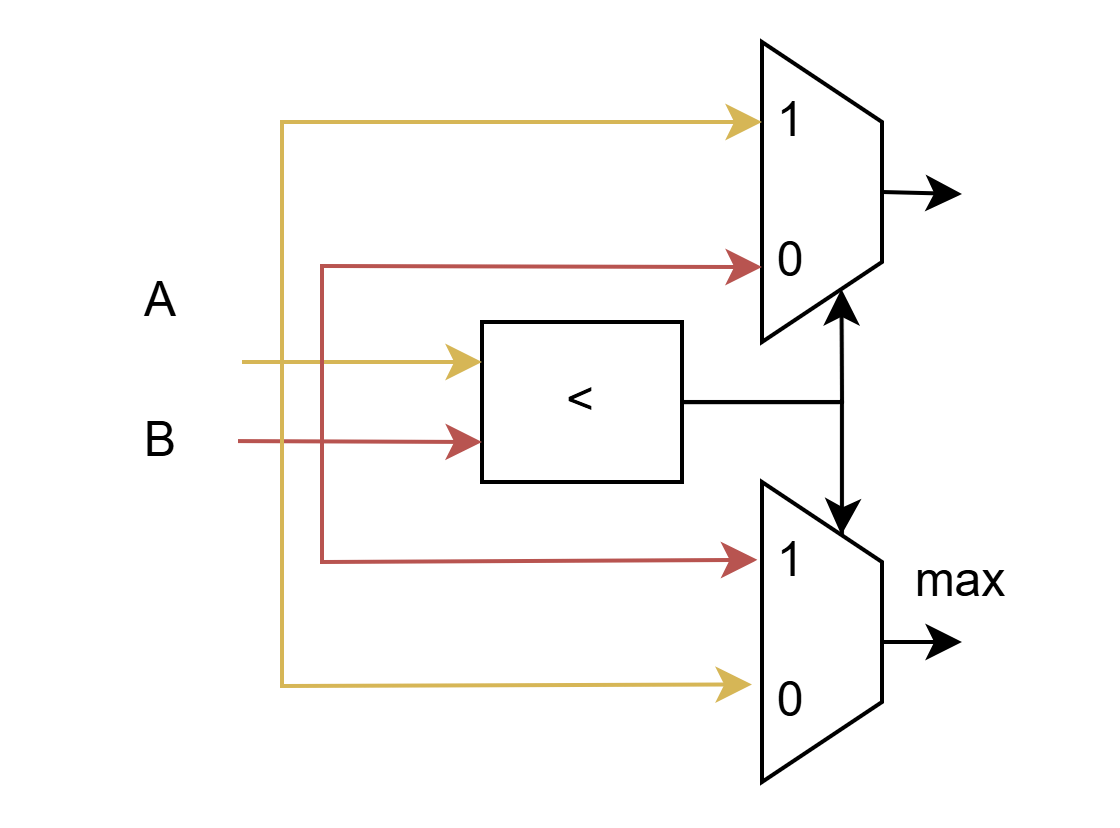
\includegraphics[width=\linewidth]{figures/node.png}
		\caption{Mô tả cấu trúc bộ so sánh và hoán đổi}
		\label{fig:node}
	\end{minipage}
\end{figure}
\subsubsection{Cửa sổ 3x3}

Hình \ref{fig:median3x3Exampel} mô tả nguyên lý và ví dụ về cách tìm giá trị trung vị của một ma trận kích thước 3x3. Với chuỗi đầu vào là 10, 9, 2, 5, 4, 3, 2, 2, 1. Giá trị trung vị ta mong đợi đạt được là 3. Các bước thực hiện bao gồm việc sắp xếp các hàng và các cột tăng dần. Sau khi đã xong hai bước trên, lúc này đường chéo gồm các phần tử 2, 4, 3. Lúc này, sẽ thực hiện sắp xếp theo thứ tự tăng dần, kết quả đạt được là 2, 3, 4. Vậy giá trị trung vị đạt được là 3, đã giống với giá trị mong đợi đạt được.  Hình \ref{fig:median3x3RTL} mô tả kiến trúc RTL của mô-đun MedianCalculation với cửa sổ 3x3. Sinh viên đã thay thế các mạng sắp xếp khi đến bước sắp xếp cột để giảm tài nguyên phần cứng sử dụng (thay bộ Sorting\_network bằng chỉ 2 Node, vì không cần đủ 3 giá trị cho bước tiếp theo), hai là đã chèn thêm các thanh ghi giữa các bước để giảm trễ lan truyền, giúp tăng tần số hoạt động của mạch.
\begin{figure}[!ht]
	\centering
	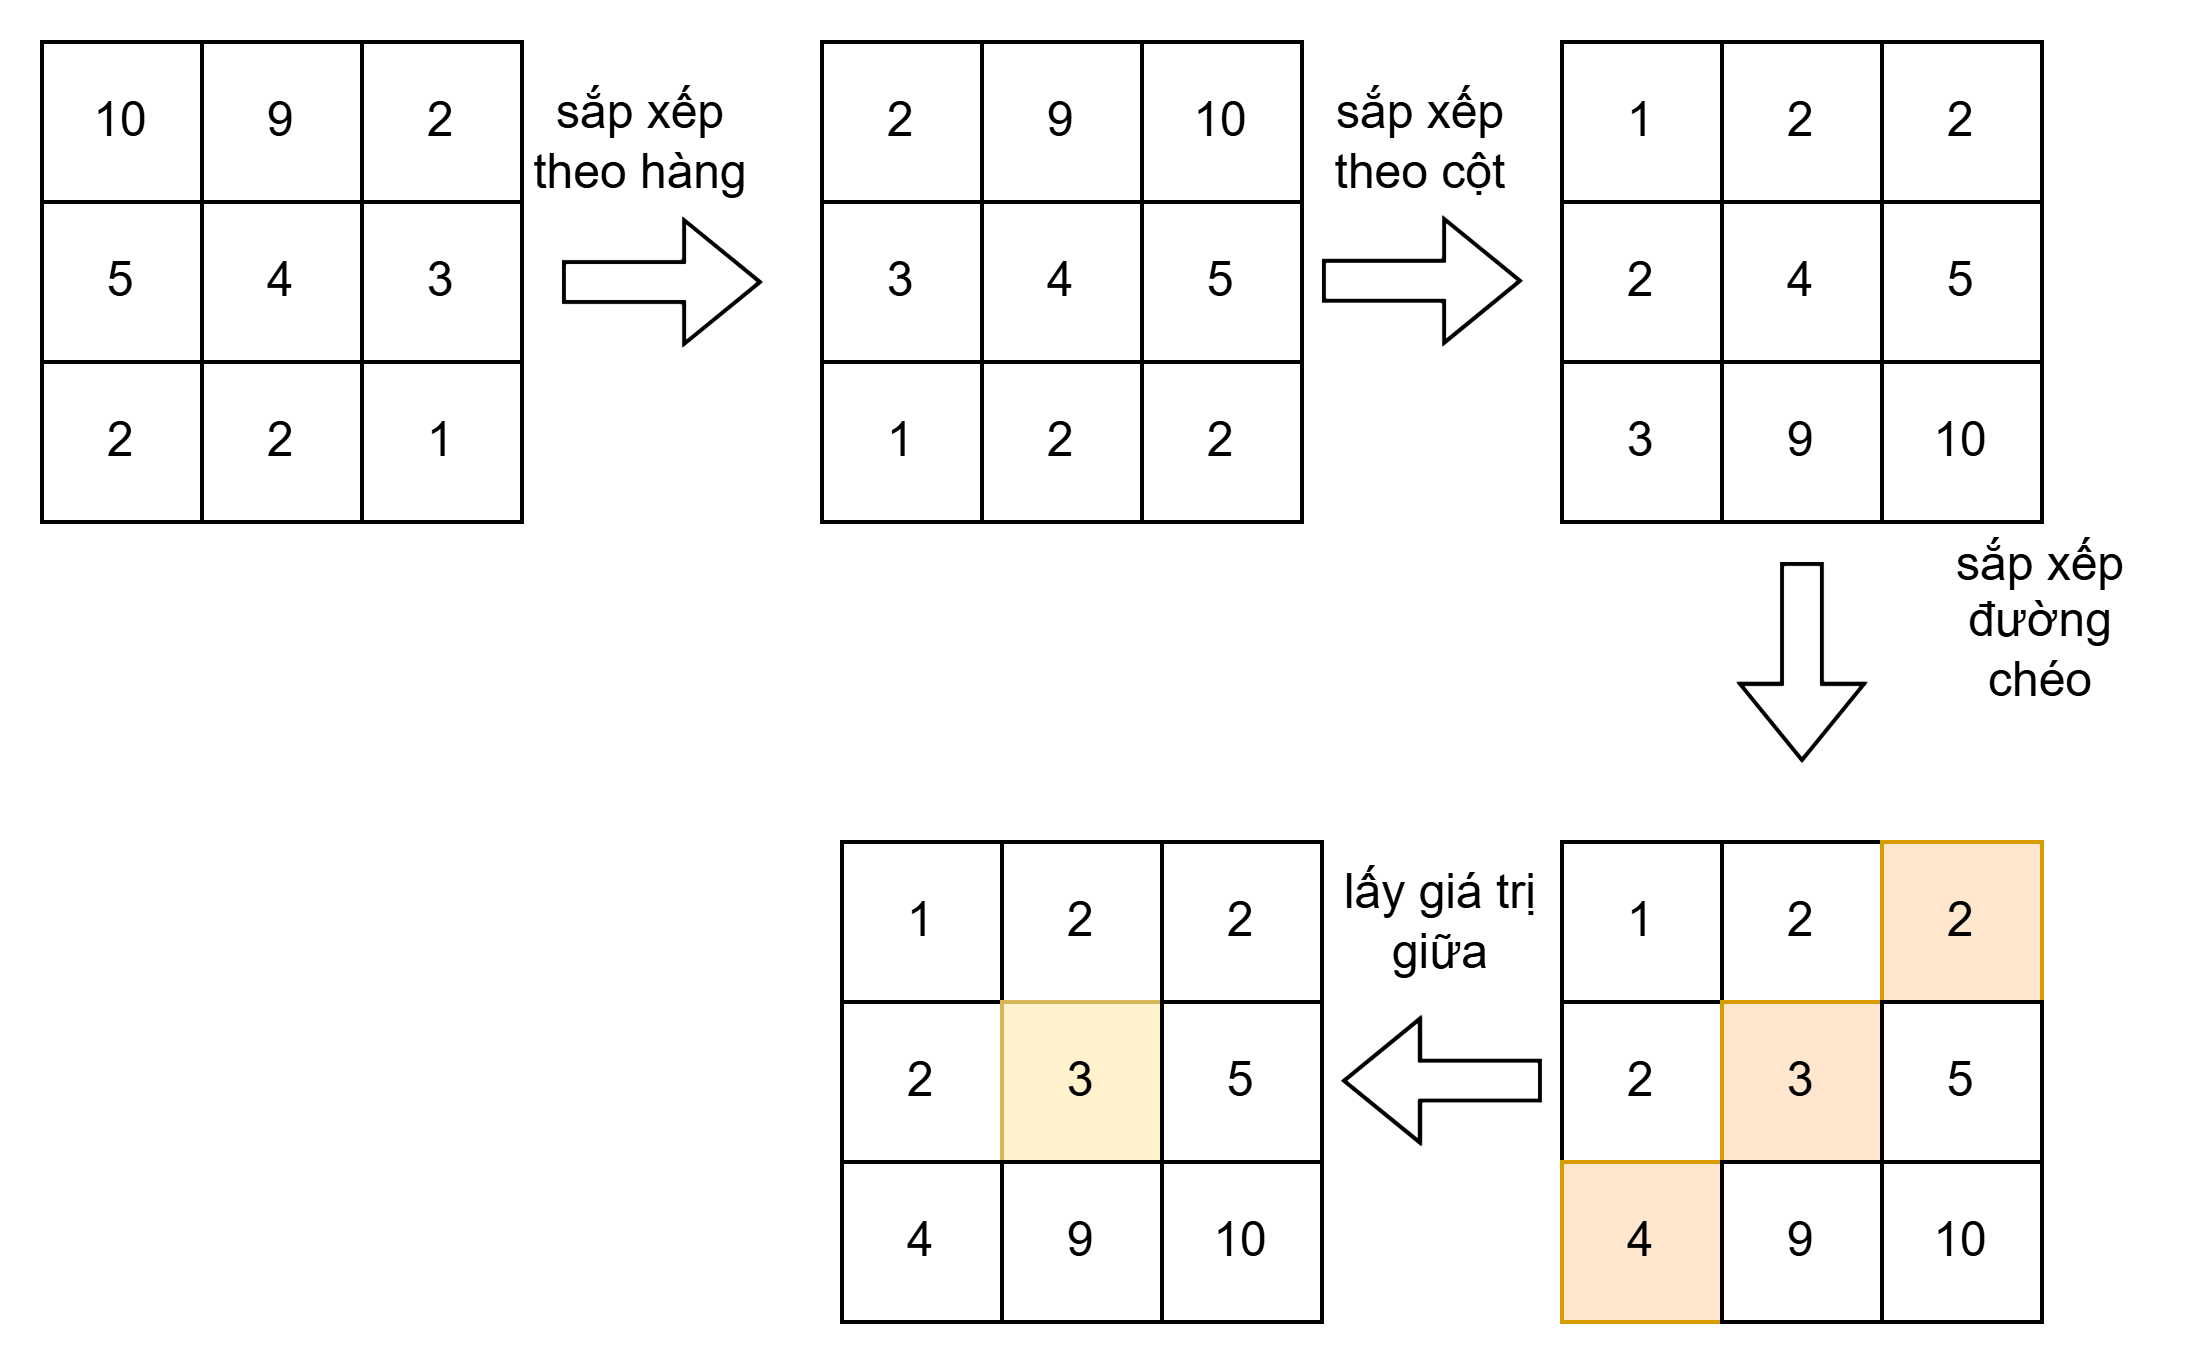
\includegraphics[width=0.6\linewidth]{figures/median3x3Exampel.png}
	\caption{Thực hiện và ví dụ của tìm trung vị của cửa sổ 3x3}
	\label{fig:median3x3Exampel}
\end{figure}
\begin{figure}[H]
	\centering
	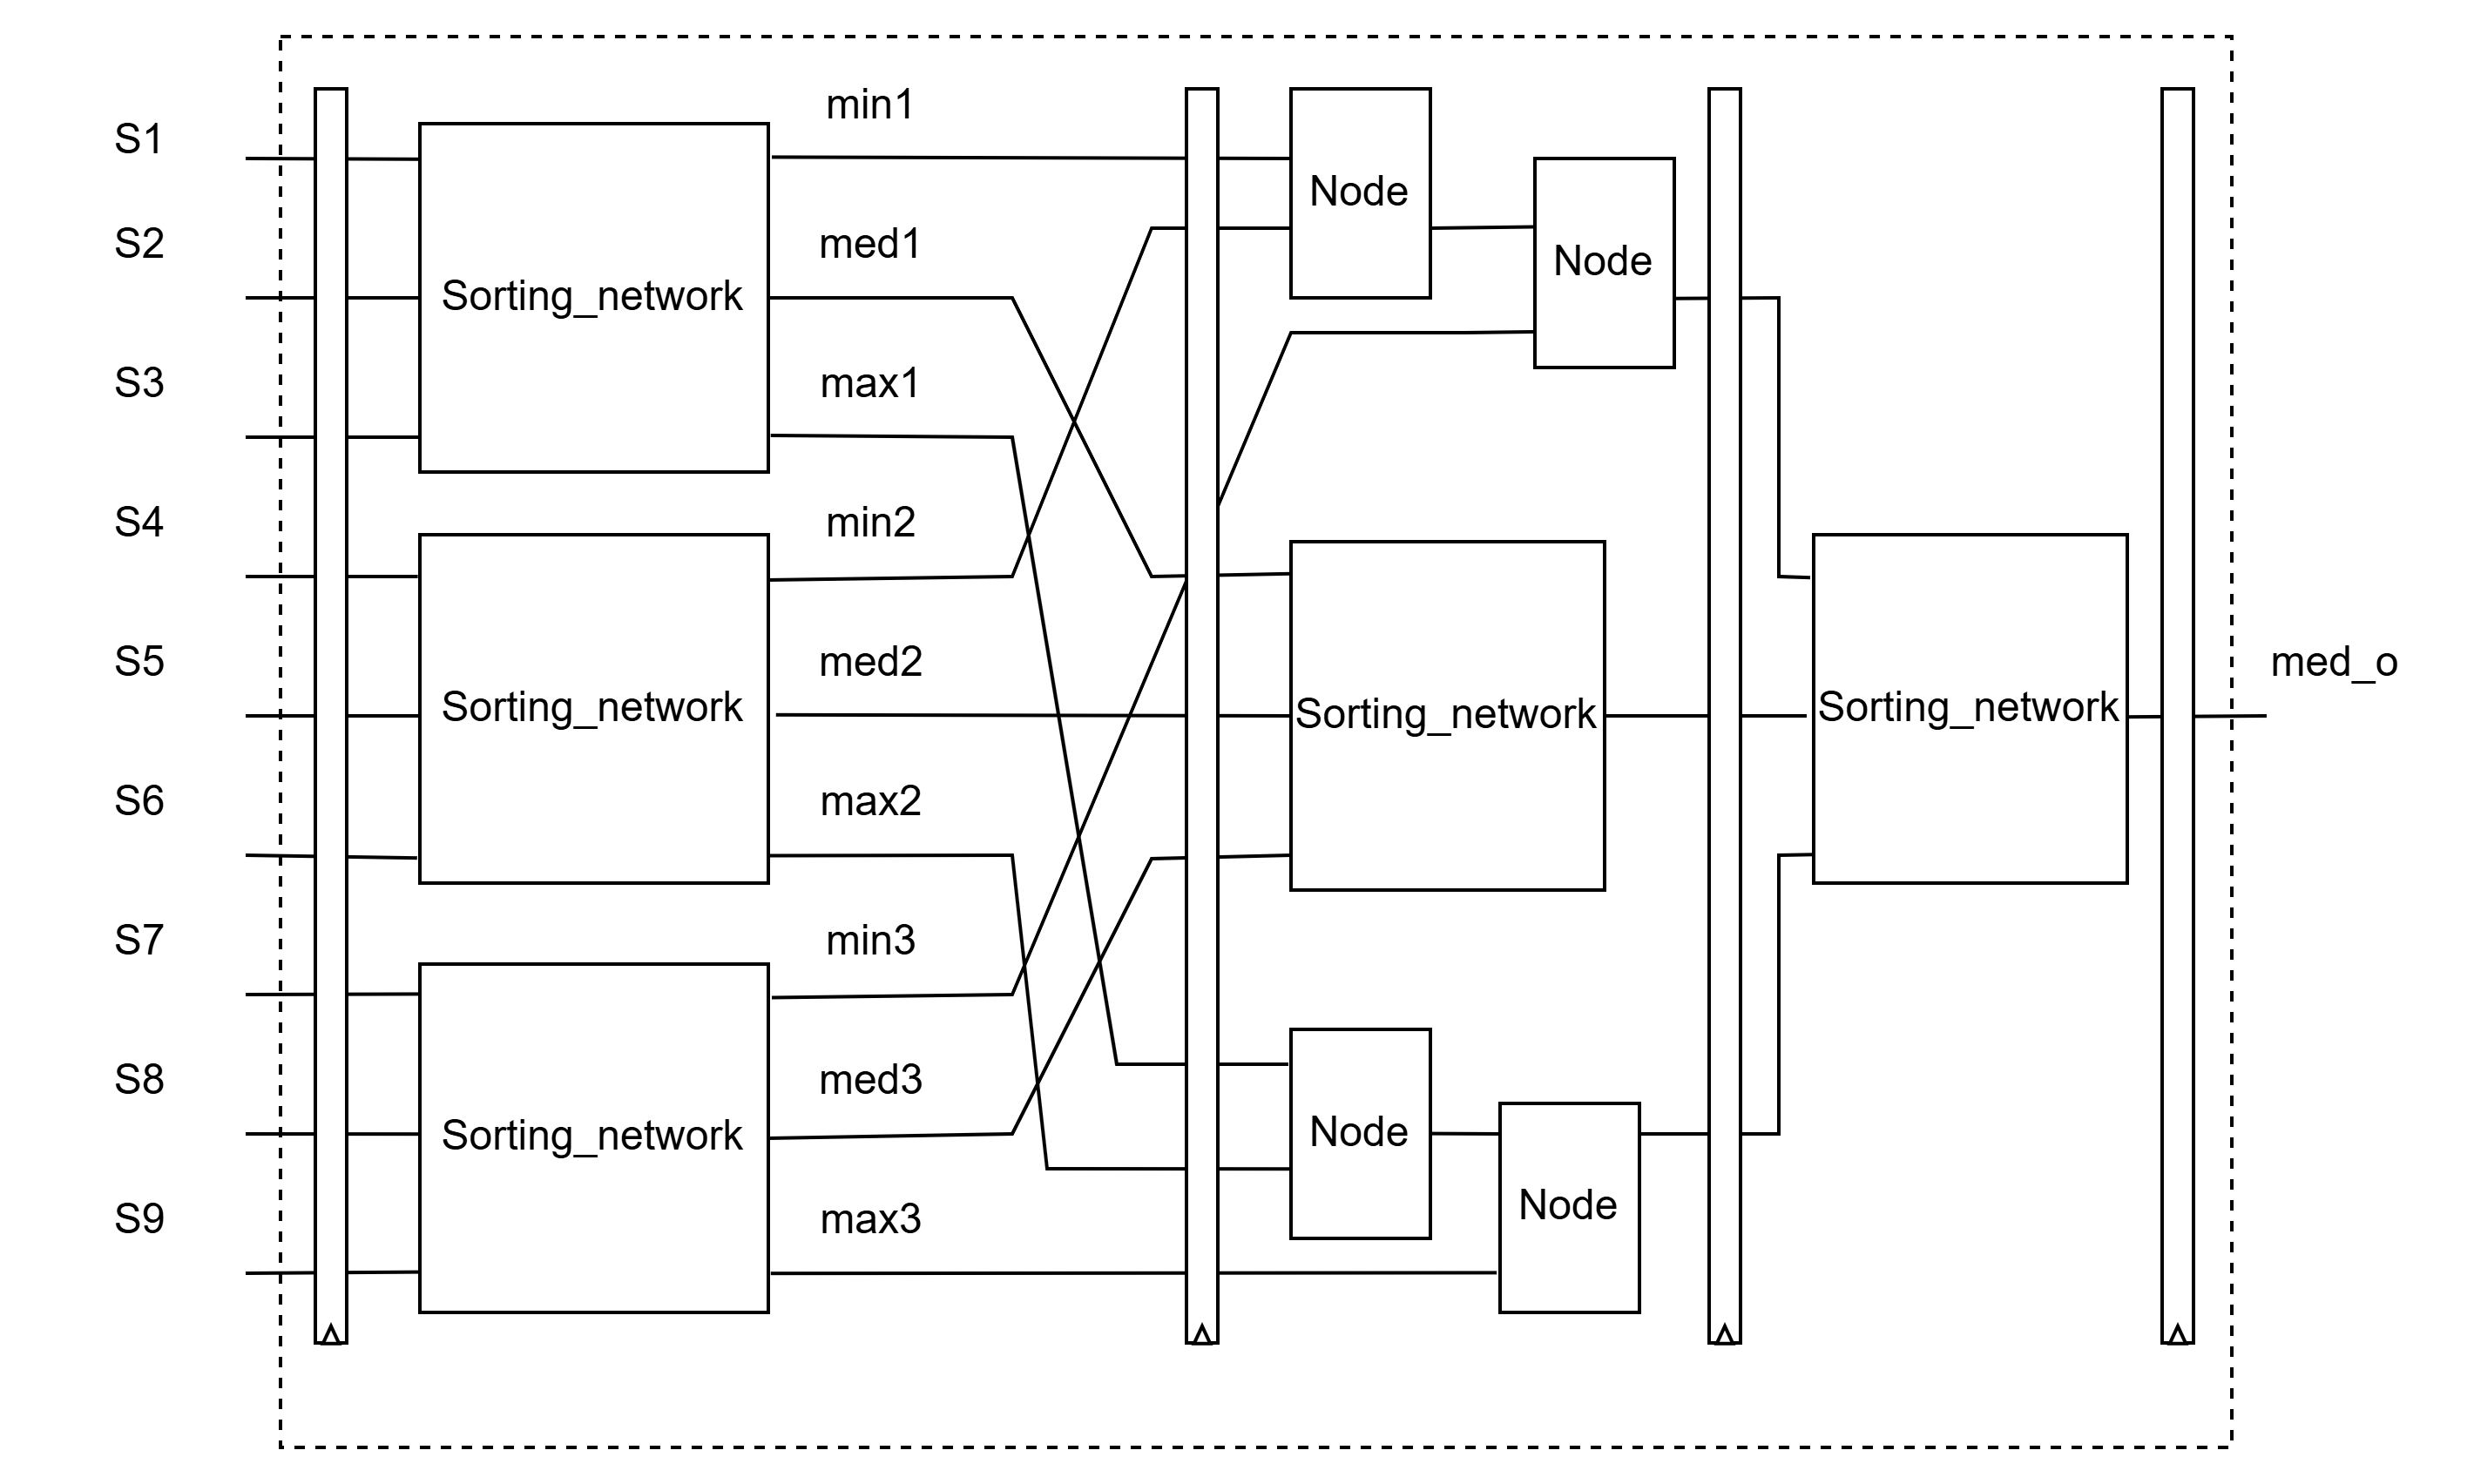
\includegraphics[width=\linewidth]{figures/median3x3RTL.png}
	\caption{Thực hiện và ví dụ của tìm trung vị của cửa sổ 3x3}
	\label{fig:median3x3RTL}
\end{figure}

\subsubsection{Cửa sổ 5x5}

Hình \ref{fig:median5x5Example} mô tả nguyên lý và ví dụ về cách tìm giá trị trung vị đối với cửa sổ 5x5. Để tối ưu cho tốc độ sắp xếp và sự không phụ thuộc, sinh viên sẽ thiết kế một sắp xếp 5 phần tử theo thứ tự tăng dần theo các bước được mô tả trong hình \ref{fig:sortAscending5x5RTL}.

\begin{figure}[!ht]
	\centering
	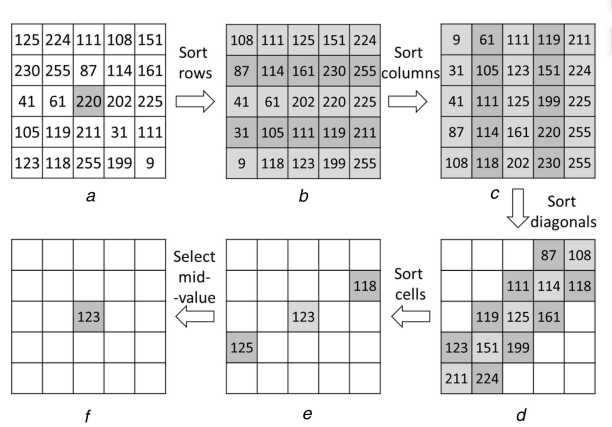
\includegraphics[width=0.8\linewidth]{figures/median5x5Example.png}
	\caption{Thực hiện và ví dụ của tìm trung vị của cửa sổ 5x5 \cite{llmf}}
	\label{fig:median5x5Example}
\end{figure}

\begin{figure}[!ht]
	\centering
	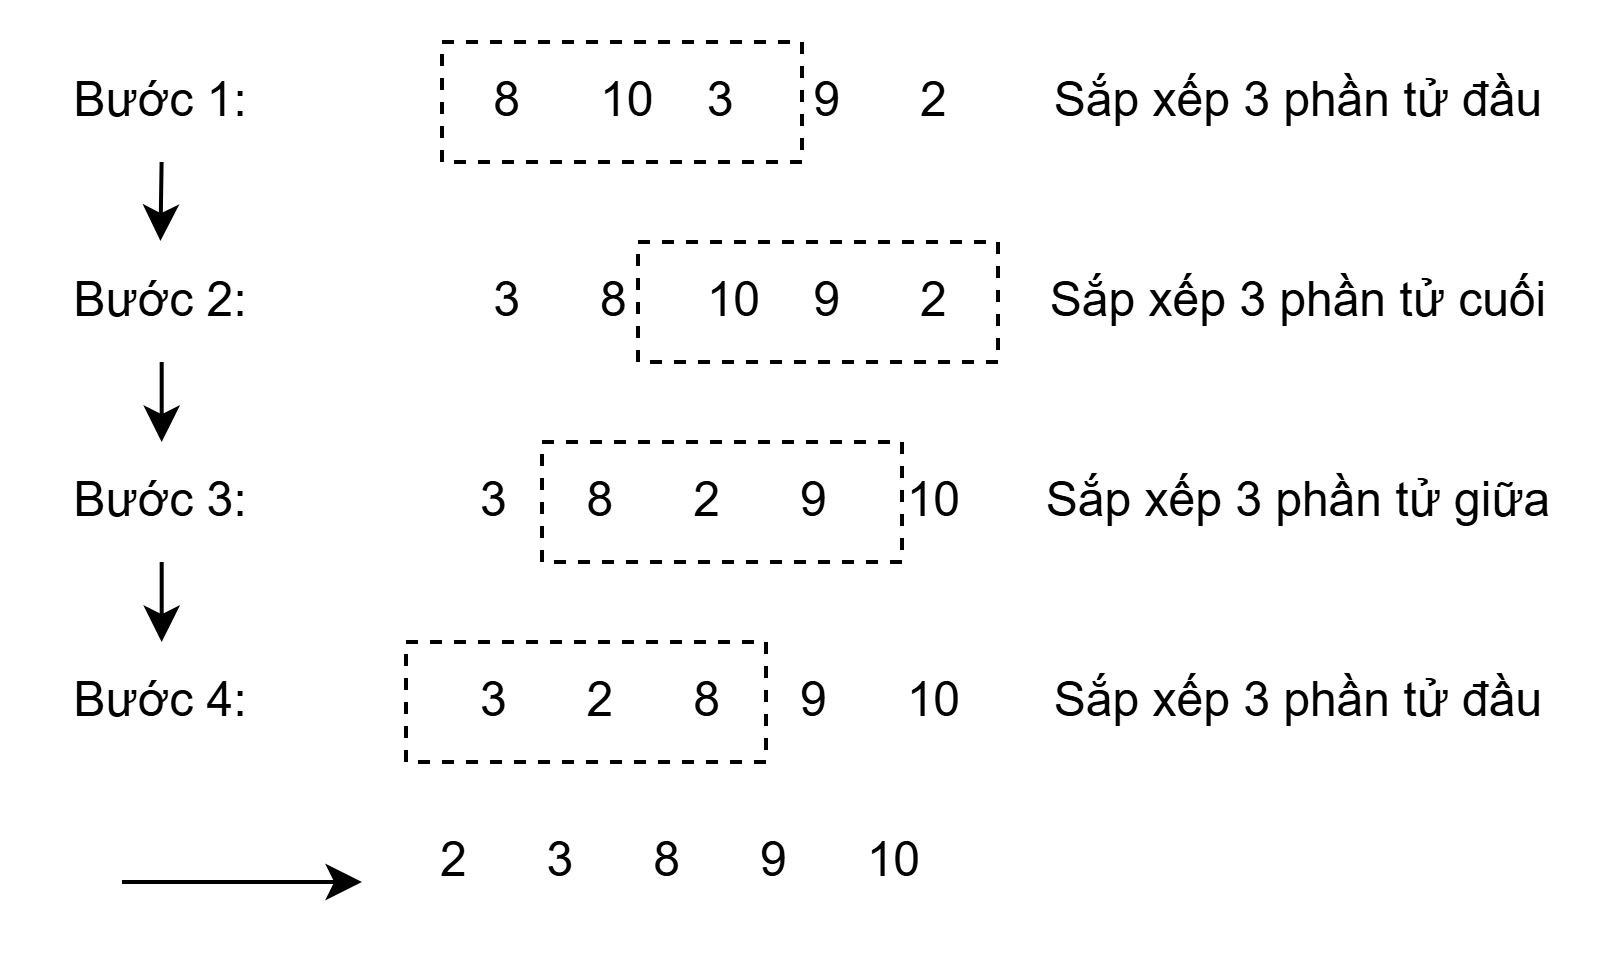
\includegraphics[width=0.8\linewidth]{figures/sortAscending5x5Ex.png}
	\caption{Xây dựng bộ sắp xếp 5 phần tử dựa trên bộ sắp xếp 3}
	\label{fig:sortAscending5x5Ex}
\end{figure}

\begin{figure}[!ht]
	\centering
	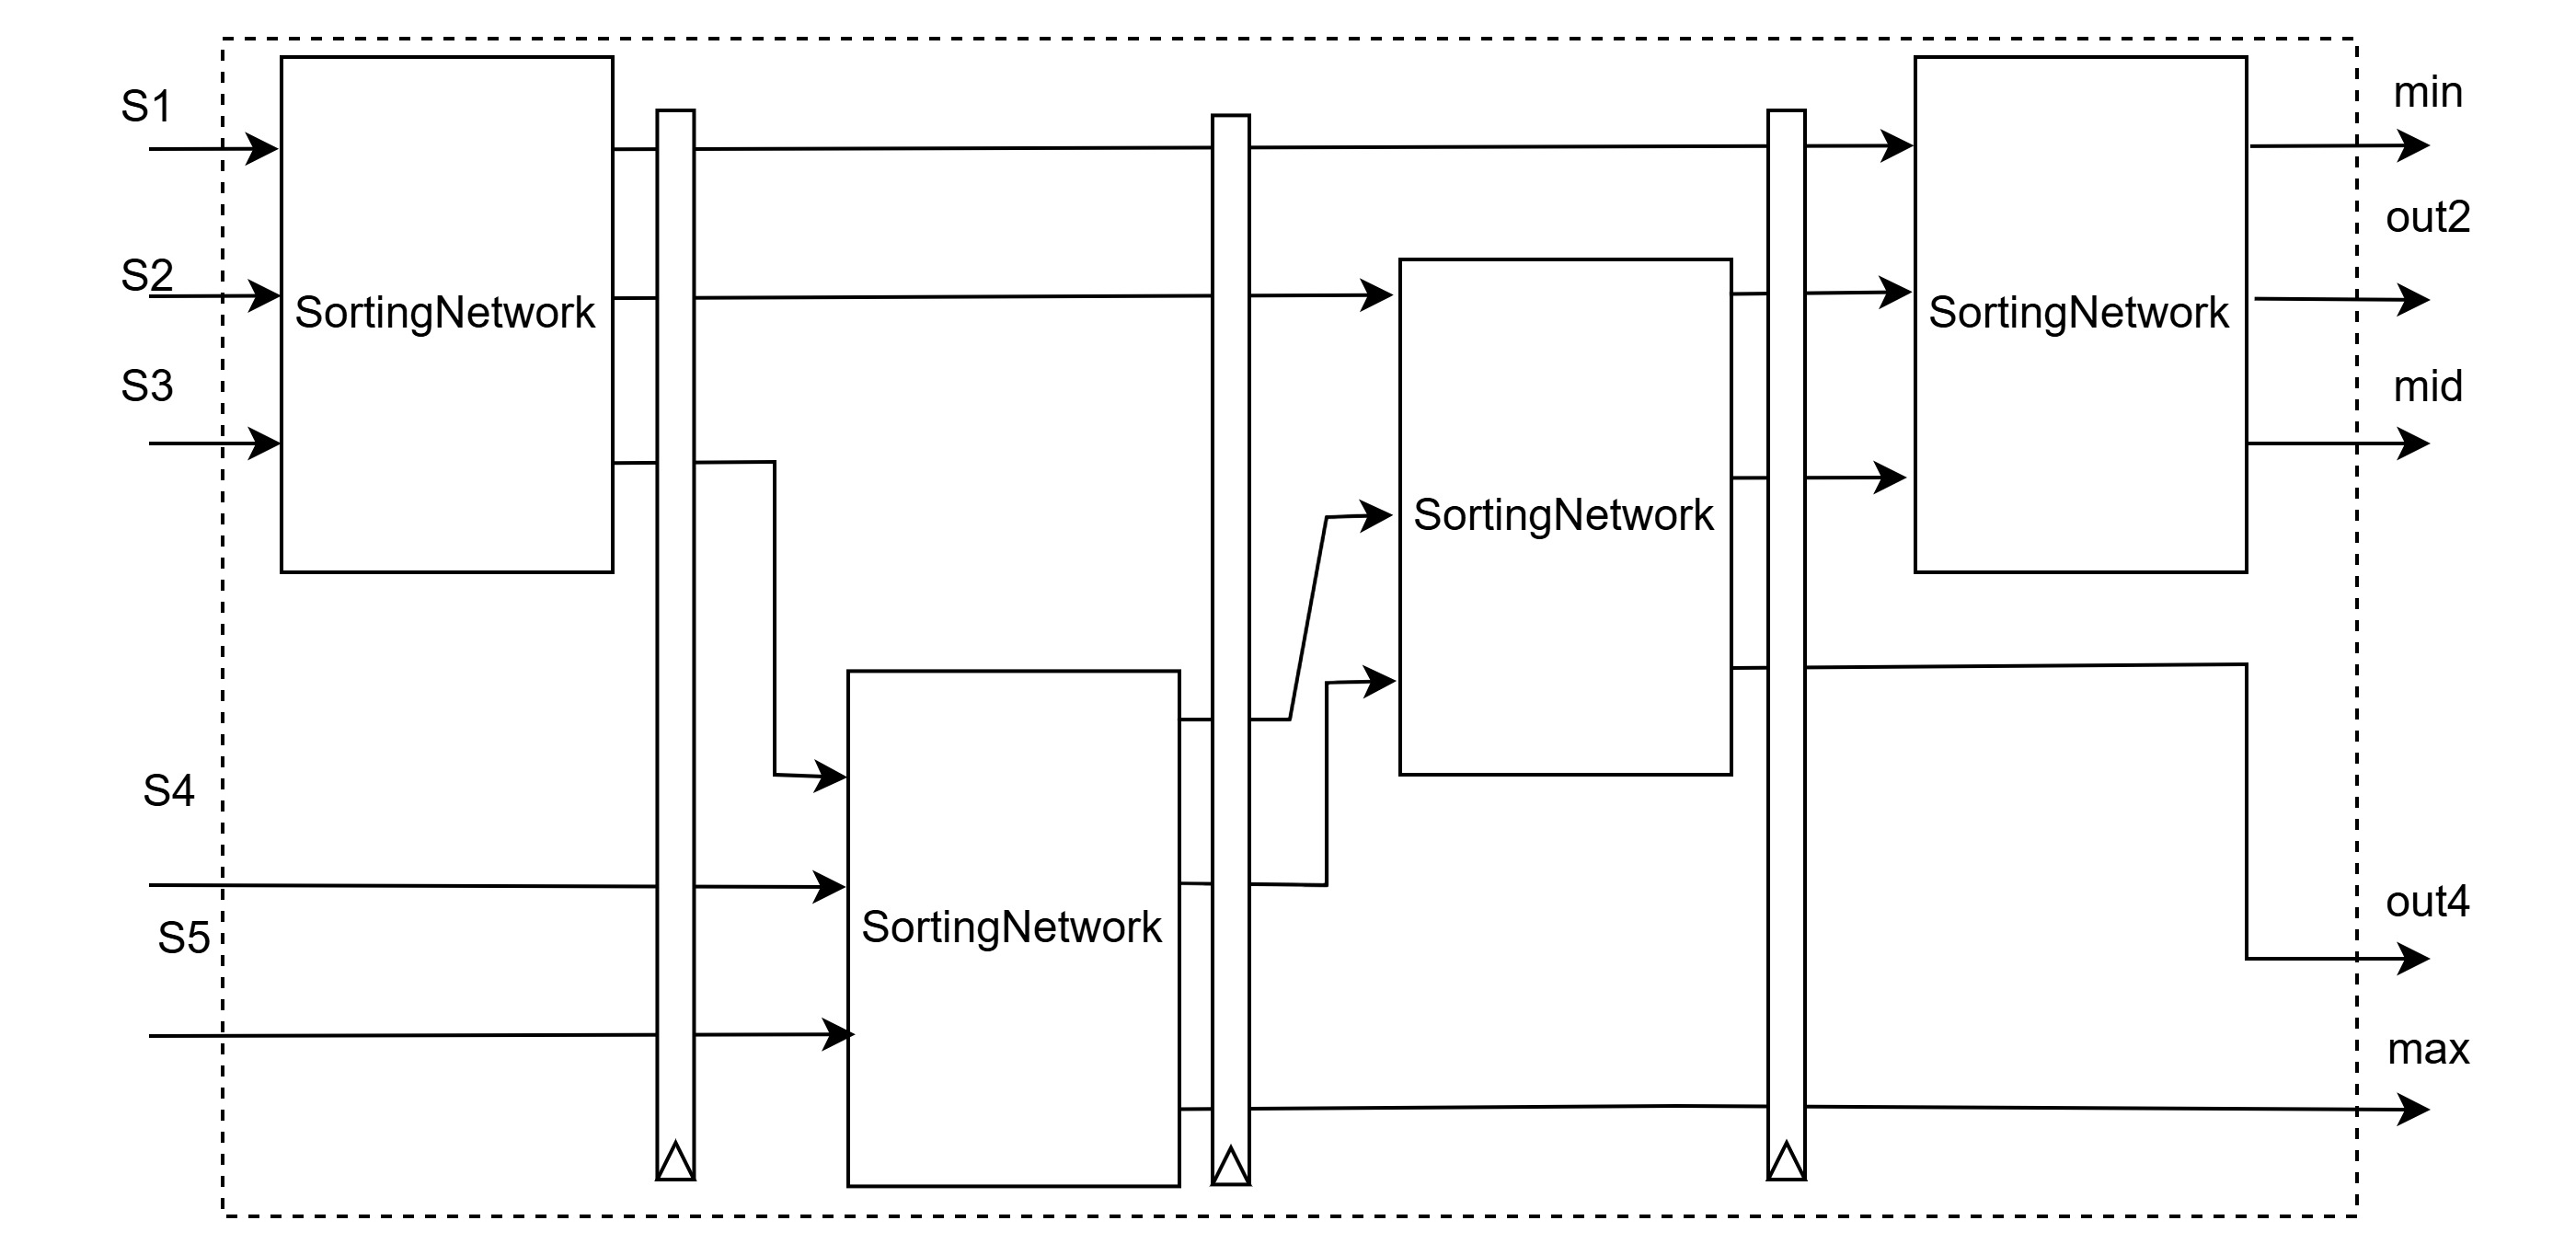
\includegraphics[width=\linewidth]{figures/sortAscending5x5RTL.png}
	\caption{Kiến trúc của bộ sắp xếp tăng dần 5 phần tử}
	\label{fig:sortAscending5x5RTL}
\end{figure}

\subsubsection{Cửa sổ 7x7}

Hình \ref{fig:median7x7Example} mô tả cách tìm ra giá trị trung vị đối với một ma trận kích thước 7x7. Điểm khác biệt đối với cửa sổ này là sau khi đã sắp xếp hàng và sắp xếp cột xong, ta sẽ tìm ra 25 phần tử thỏa mãn điều kiện, sau đó dựa vào bộ tìm trung vị đối với ma trận 5x5 để tìm trung vị chứ không thực hiện trực tiếp việc sắp xếp đường chéo theo mô tả tại thuật toán \ref{alg:medianFilterAlgo}. Sau khi sắp xếp theo hàng và cột xong, giá trị tại các ô xanh trong hình \ref{fig:median7x7Example} đã thỏa mãn điều kiện, tuy nhiên ở mỗi góc sẽ tồn tại 3 giá trị như mô tả tại ô màu vàng. Đối với phía trên, ta cần tìm giá trị lớn nhất của nó và đối với phía dưới, ta cần tìm giá trị nhỏ nhất. Từ đó, ta sẽ có đủ 25 phần tử và sử dụng nó có thể tìm kiếm được giá trị trung vị.

Để thực hiện sắp xếp tăng dần cho một cửa sổ 7x7, ta cần bộ sắp xếp tăng dần cho 7 phần tử, nó có thể được xây dựng trên các bộ sắp xếp 5 và bộ sắp xếp 3.


\begin{table}[H]
	\centering
	\renewcommand{\arraystretch}{1.3}
		\caption{Số chu kỳ thực hiện của các mô-đun mô-đun sắp xếp và mô-đun MedianCalculation}
	\begin{tabular}{|p{5cm} p{5cm} |}
		\hline
		\rowcolor{gray!30}
		\textbf{Tên mô-đun} & \textbf{Số chu kỳ}
		\\ \hline
		Bộ sắp xếp 3 phần tử & 1 chu kỳ
		  \\
		\hline
		MedianCalculation3x3  & \textbf{4 chu kỳ}
		\\ \hline
		Bộ sắp xếp 5 phần tử & 3 chu kỳ
		\\ \hline
		MedianCalculation5x5 & \textbf{14 chu kỳ}
			\\ \hline
		Bộ sắp xếp 7 phần tử & 9 chu kỳ
		\\ \hline
		MedianCalculation7x7 & \textbf{35 chu kỳ}
		\\ \hline
	\end{tabular}

	\label{tab:numberOfCycleMedianCalculation}
\end{table}

\begin{figure}[!ht]
	\centering
	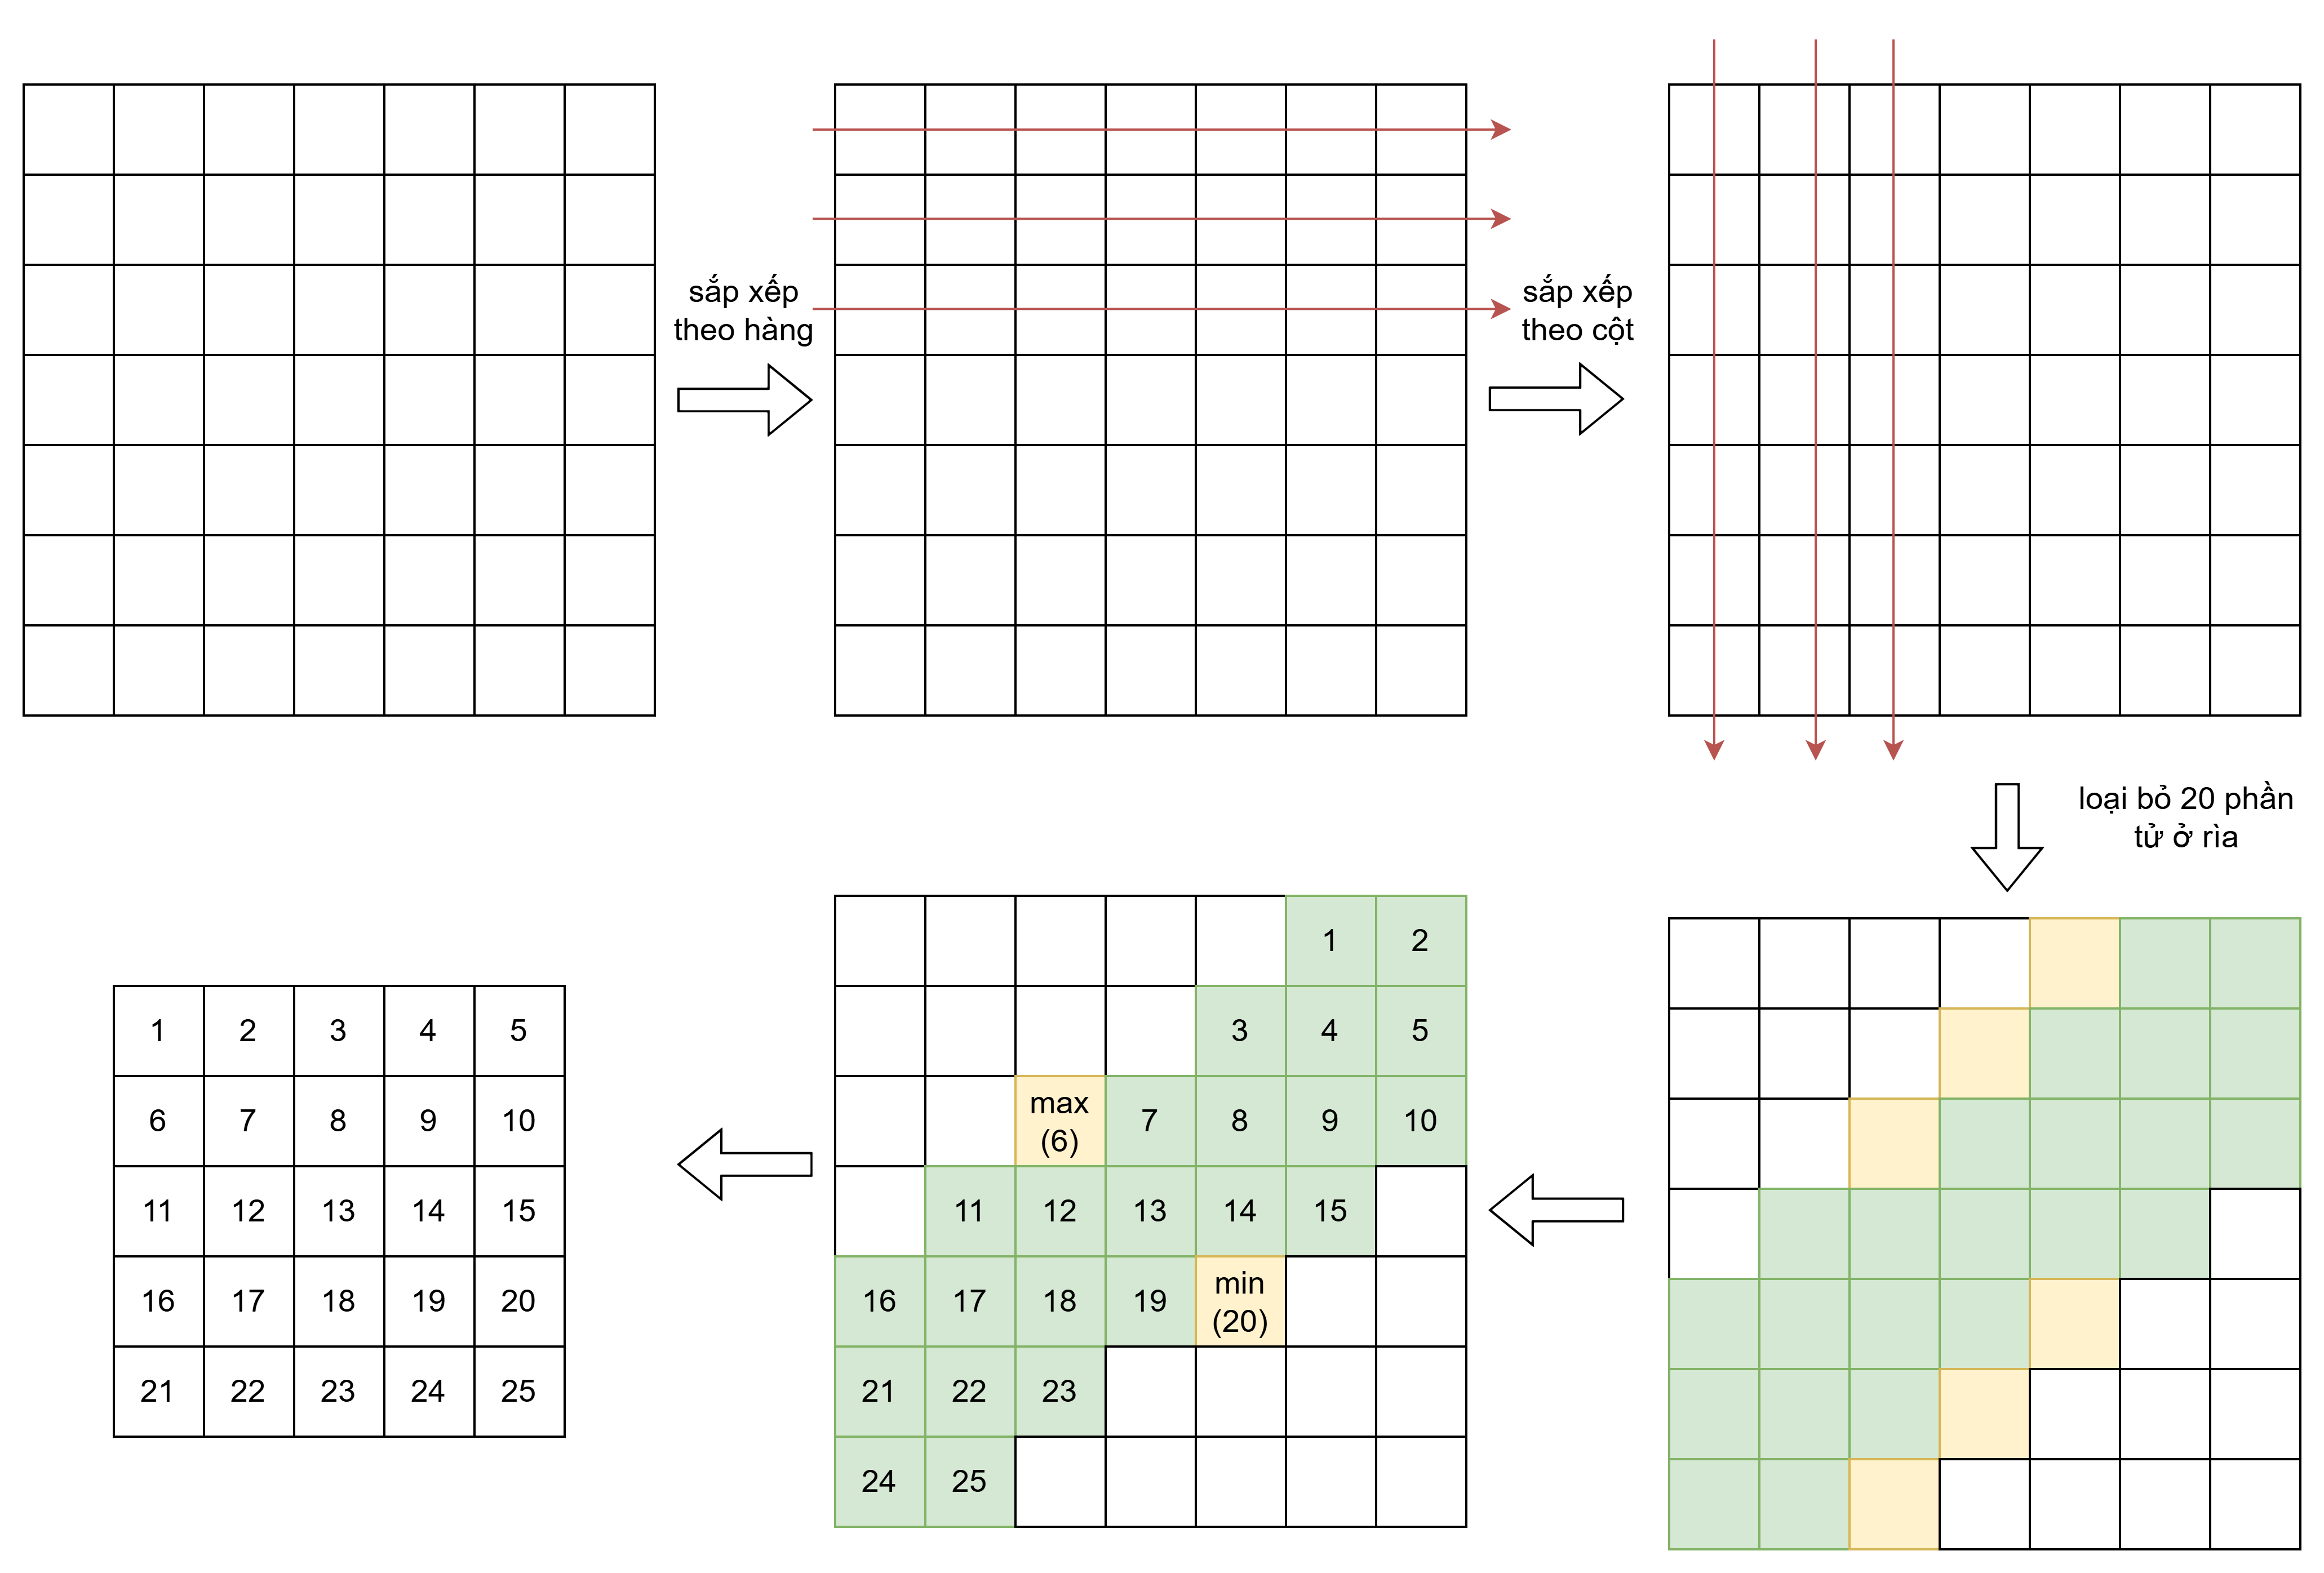
\includegraphics[width=\linewidth]{figures/median7x7Example.png}
	\caption{Thực hiện và ví dụ của tìm trung vị của cửa sổ 7x7}
	\label{fig:median7x7Example}
\end{figure}
\begin{figure}[!ht]
	\centering
	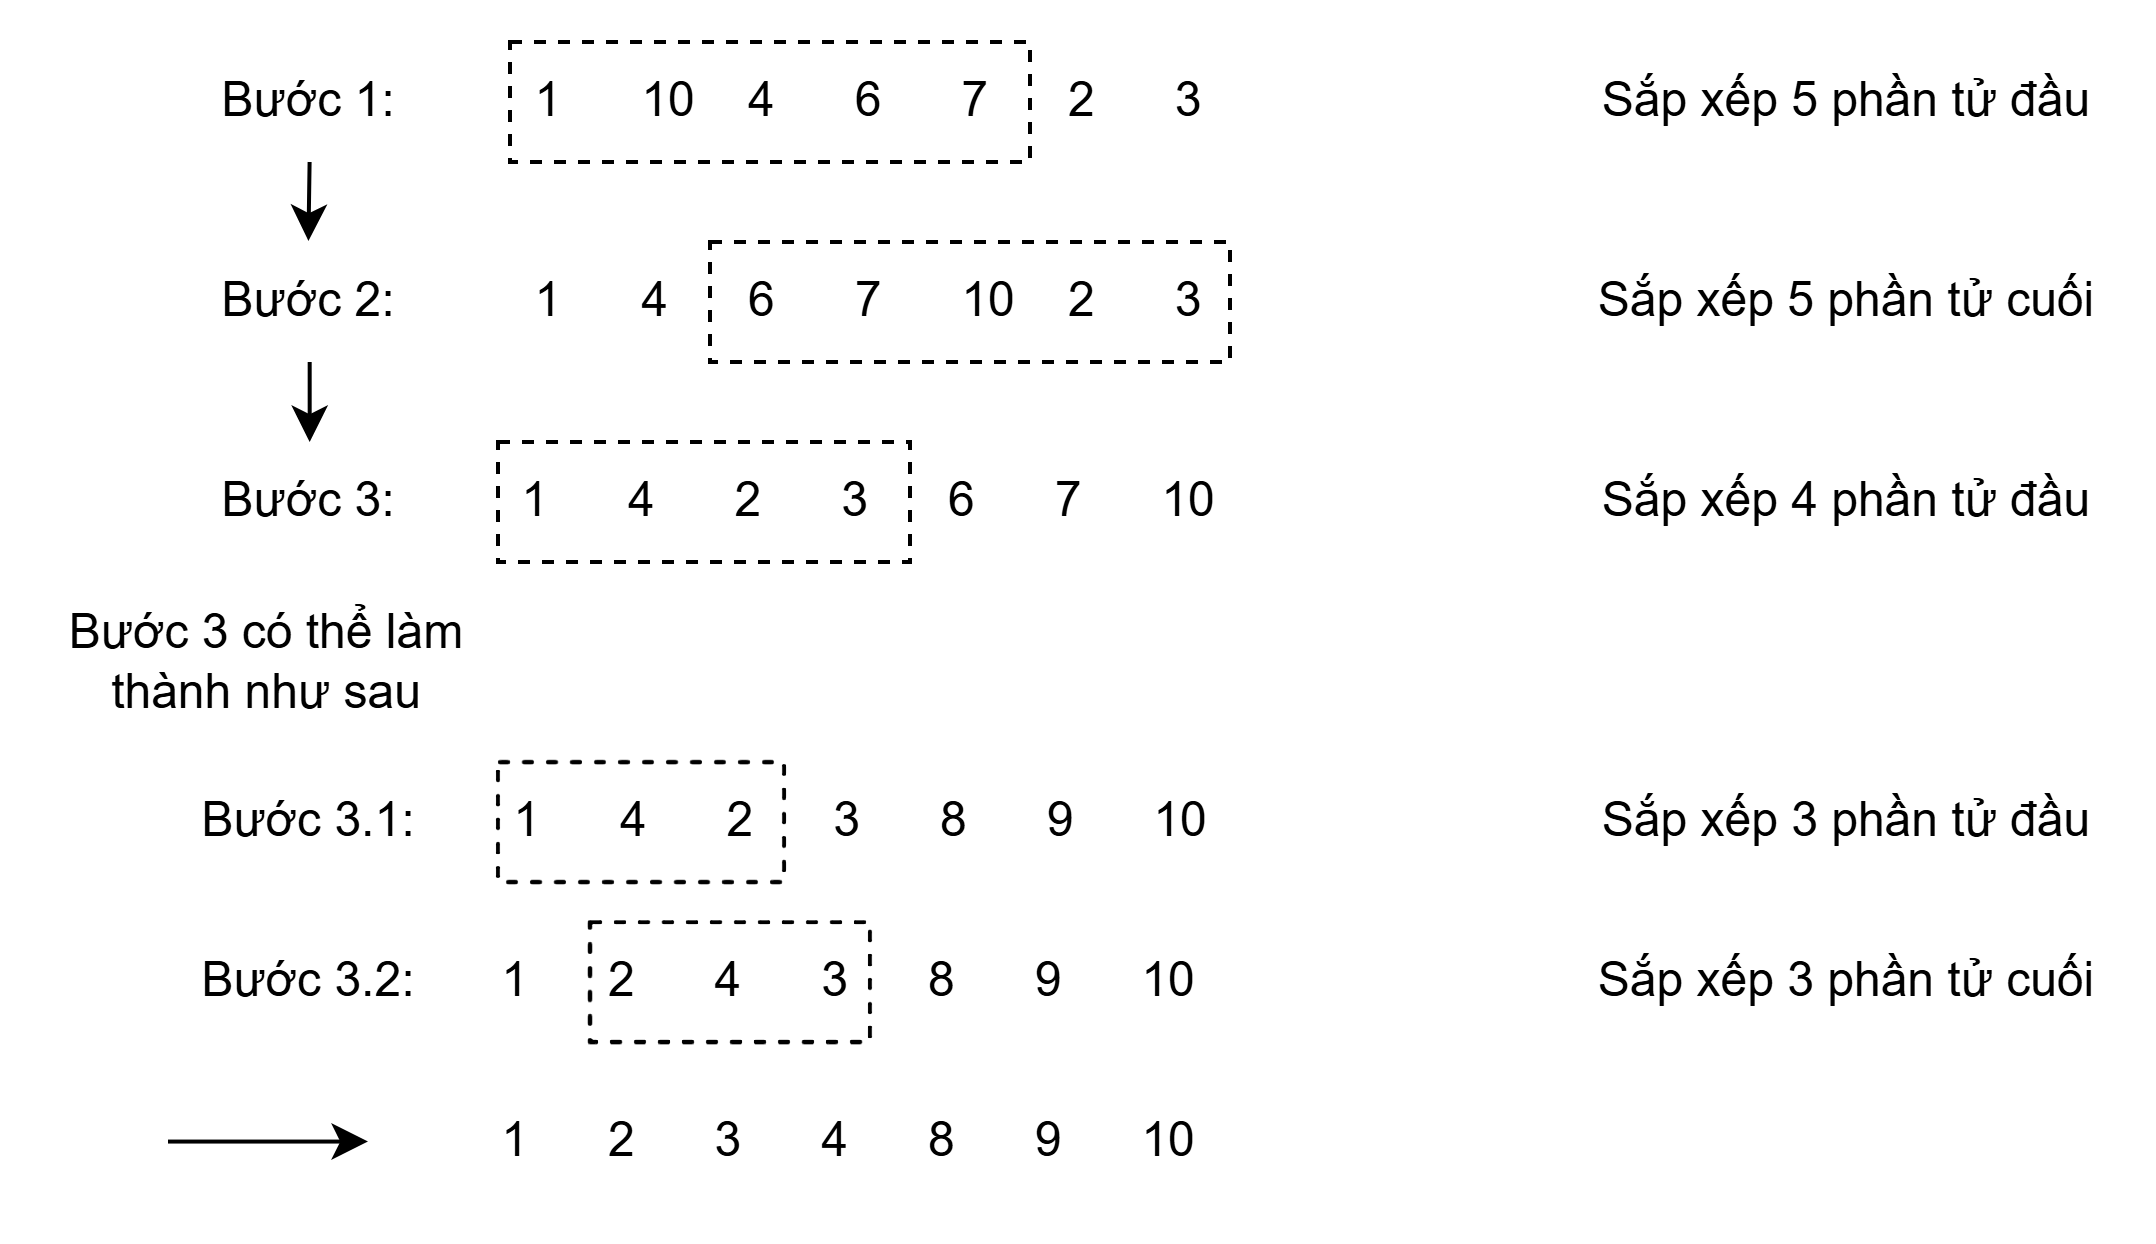
\includegraphics[width=0.8\linewidth]{figures/sortAscending7x7Ex.png}
	\caption{Xây dựng bộ sắp xếp 7 phần tử dựa trên bộ sắp xếp 5 và bộ sắp xếp 3}
	\label{fig:sortAscending7x7Ex}
\end{figure}

\section{mô-đun CI}
mô-đun CI thực chất là tập hợp của các 3 mô-đun MRELBP\_CI, trong mỗi mô-đun đó là khối PatchSum nối với một mạch logic tổ hợp để nhằm mục đích so sánh và đưa ra giá trị so sánh đối với các phần tử trung tâm của một cửa sổ. Về cơ bản 3 mô-đun PatchSum đều xây dựng trên nguyên tắc chung sẽ được trình bày tại phần ngay sau.
\subsection{Cơ sở xây dựng mô-đun PatchSum}
Một cách đơn giản nhất để tính tổng của các cửa sổ là cộng tất cả các giá trị trong cửa sổ lại với nhau, nếu với cửa sổ kích thước 5x5, ta sẽ cần cộng khoảng 25 giá trị trong 1 chu kỳ (nếu không sử dụng phương pháp đường ống), hoặc thực hiện một bộ cộng tuần tự, tuy nhiên nó sẽ giảm khả năng xử lý thời gian thực. Để giải quyết vấn đề này, sinh viên sẽ thực hiện một kỹ thuật triển khai giống với cửa sổ trượt. Hình \ref{fig:slidingWindowPrincipla} mô tả một ví dụ về kỹ thuật cửa sổ trượt. Cửa sổ mà có viền màu đỏ là cửa sổ ban đầu. Cửa sổ mà có viền màu xanh là cửa sổ ngay sau cửa sổ màu đỏ. Ta thấy, tổng của 2 cửa sổ này đều có một đặc điểm là có các giá trị ở các ô màu vàng. Giá trị tổng của cửa sổ sau sẽ bằng giá trị của cửa sổ trước đó trừ đi giá trị ở các ô màu đỏ và cộng với các giá trị ở các ô màu xanh. Bằng nguyên lý đó, ta có thể giảm bớt số lượng phép cộng cần thực hiện trong 1 chu kỳ.


\begin{figure}[!ht]
	\centering
	\begin{minipage}[t]{0.48\linewidth}
		\centering
		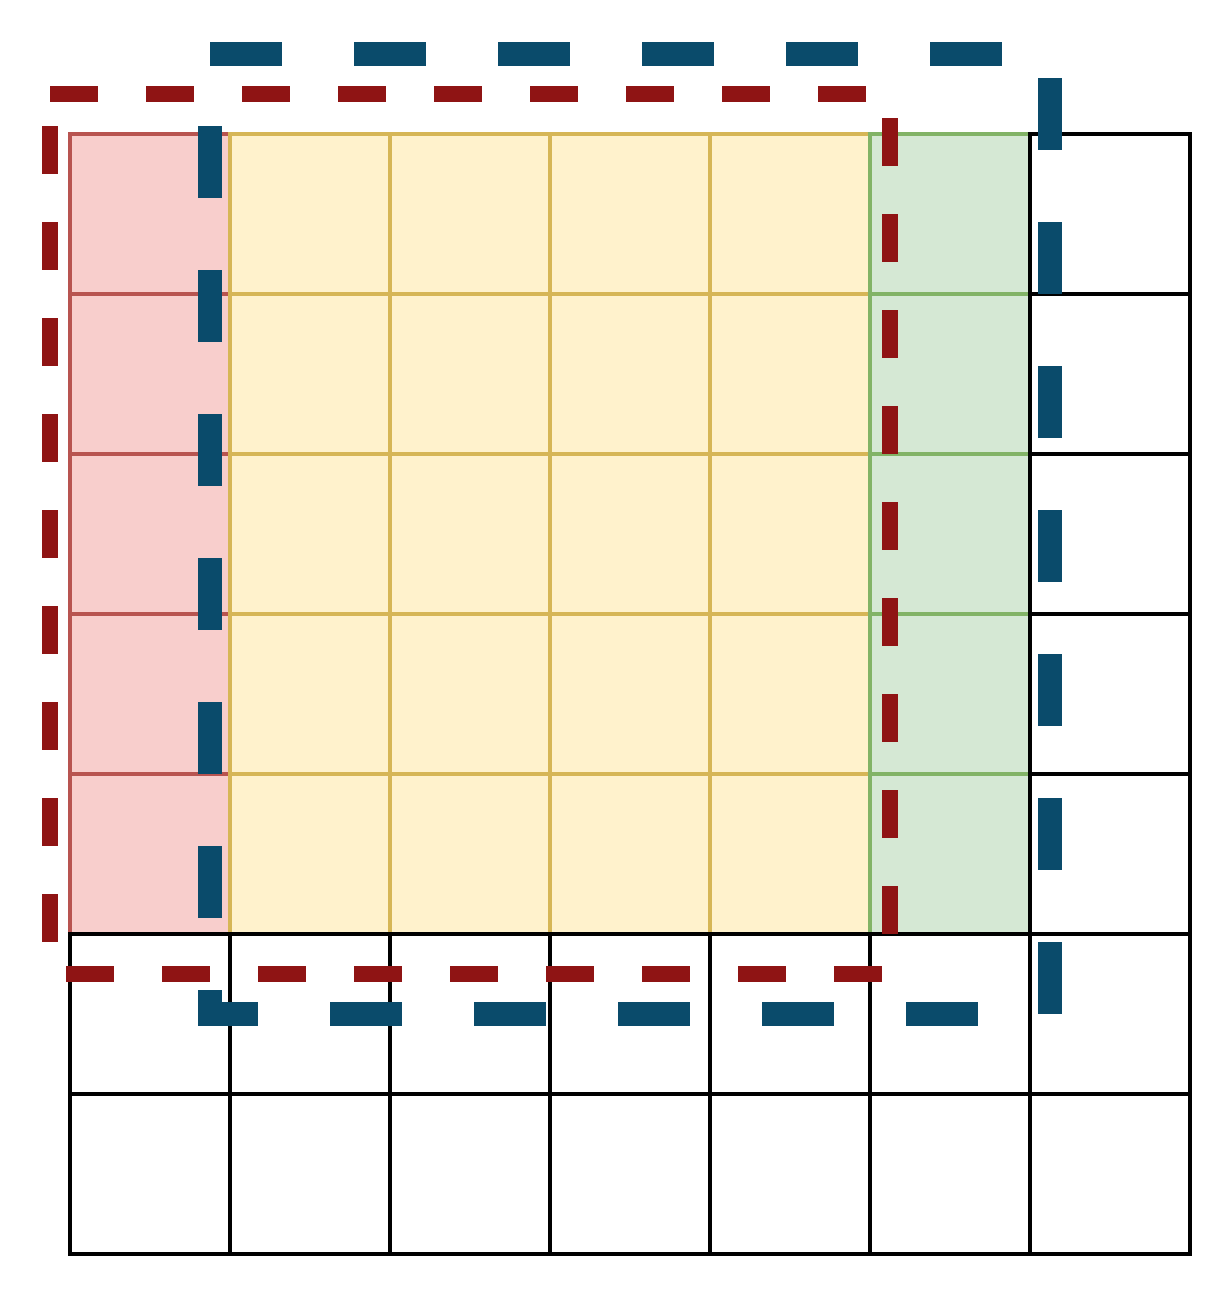
\includegraphics[width=\linewidth]{figures/slidingWindowPrincipla.png}
		\caption{Ví dụ về nguyên lý cửa kỹ thuật cửa sổ trượt}
		\label{fig:slidingWindowPrincipla}
	\end{minipage}
	\hfill
	\begin{minipage}[t]{0.48\linewidth}
		\centering
		\includegraphics[width=\linewidth]{figures/sumCumRTL.png}
		\caption{Kiến trúc của mô-đun sum\_cum}
		\label{fig:sumCumRTL}
	\end{minipage}
\end{figure}



\subsection{Xây dựng mô-đun PatchSum}
\subsubsection{Sơ đồ chuyển trạng thái}
Vì sẽ xây dựng 3 mô-đun PatchSum ứng với 3 giá trị bán kính r khác nhau, tuy nhiên cả 3 mô-đun này đều có cùng 1 nguyên lý hoạt động, do đó sinh viên sẽ xây dựng chung 1 bộ sơ đồ chuyển trạng thái, được mô tả tại hình \ref{fig:patchSumTrans}. 

\begin{figure}[!ht]
	\centering
	\includegraphics[width=0.8\linewidth]{figures/patchSumTrans.png}
	\caption{Sơ đồ chuyển trạng thái của mô-đun PatchSum}
	\label{fig:patchSumTrans}
\end{figure}
\subsubsection{Kiến trúc RTL}
Hình \ref{fig:patchSumRTL} mô tả kiến trúc RTL chung của cả 3 bộ PatchSum ứng với các bán kính r = 2, 4, 6. Đây là các bộ giúp kiểm tra các điều kiện để máy trạng thái chuyển trạng thái, cả 3 mô-đun ứng với 3 loại r khác nhau đều sử dụng các bộ này, tuy nhiên thì mỗi bán kính sẽ ứng với các điều kiện khác nhau và các điều kiện Condition sẽ được mô tả tại bảng \ref{tab:conditionRTLPatchSum}. Một mô PatchSum ứng với một giá trị r cụ thể sẽ có mô tả RTL ở cả 2 hình \ref{fig:patchSumRTL} và \ref{fig:patchSumRTL_2}. Tuy nhiên hình \ref{fig:patchSumRTL_2} là mô tả RTL đầu ra cho mô-đun PatchSum với r = 2, với r = 4 và r = 6, kiến trúc sẽ có sự khác biệt về số lượng thanh ghi, số chu kỳ thực hiện, nhưng về nguyên lý hoạt động là tương tự nhau. Hình \ref{fig:sumCumRTL} mô tả cấu trúc của mô-đun sum\_cum được sử dụng ở cuối kiến trúc RTL (2) của mô-đun PatchSum.
\begin{table}[H]
	\centering
		\caption{Bảng điều kiện cho mô tả hình \ref{fig:patchSumRTL}}
	\begin{tabular}{|>{\centering\arraybackslash}m{5cm}|>{\centering\arraybackslash}m{3cm}|>{\centering\arraybackslash}m{3cm}|>{\centering\arraybackslash}m{3cm}|}
		\hline
		\rowcolor{gray!30}
		\diagbox[width=5cm,height=1.5cm,dir=NE]{\textbf{Loại điều kiện}}{\textbf{Bán kính}} & \textbf{r = 2}  & \textbf{r = 4} & \textbf{r = 6} \\
		\hline
		Condition1 & > 3 & > 7 & > 11 \\
		\hline
		Condition2 & COLS - 2 & COLS - 2 & COLS - 2 \\
		\hline
		Condition3 & > 1 & > 2 & > 2 \\
		\hline
		Condition4 & ROWS - 4 & ROWS - 8 & ROWS - 12 \\
		\hline
	\end{tabular}

	\label{tab:conditionRTLPatchSum}
\end{table}

\begin{figure}[!ht]
	\centering
	\includegraphics[width=\linewidth]{figures/patchSumRTL.png}
	\caption{Kiến trúc RTL (1) của mô-đun PatchSum}
	\label{fig:patchSumRTL}
\end{figure}
\begin{figure}[!ht]
	\centering
	\includegraphics[width=1\linewidth]{figures/patchSumRTL_2.png}
	\caption{Kiến trúc RTL (2) của mô-đun PatchSum với r = 2}
	\label{fig:patchSumRTL_2}
\end{figure}

\section{mô-đun NIRD}
mô-đun NIRD có sơ đồ khối được mô tả theo hình \ref{fig:nirdArch} bao gồm khá nhiều mô-đun con, tuy nhiên các thành phần đó đã được mô tả một phần ở các nội dung trước, do đó trong phần này, sinh viên sẽ trình bày về kiến trúc RTL của các mô-đun con bao gồm mô-đun \textbf{Interpolation}, mô-đun \textbf{RIU2}.
\subsection{mô-đun Interpolation}
Để nội suy ra các giá trị cần thiết trong ảnh, thiết kế sẽ sử dụng phương pháp nội suy tuyến tính. Phương pháp này sẽ tính toán giá trị một điểm dựa trên 4 điểm bên ngoài. 
\begin{figure}[!ht]
	\centering
	\includegraphics[width=1\linewidth]{figures/BilinearInterpolation_fig001.png.jpg}
	\caption{Nội suy tuyến tính}
	\label{fig:BilinearInterpolationV2}
\end{figure}


Giá trị của điểm cần tính sẽ theo công thức:
\begin{equation}
	\begin{aligned}
		f(x, y) =\ &P(1,1) \cdot \frac{(x_2 - x)(y_2 - y)}{(x_2 - x_1)(y_2 - y_1)} + P(2,1) \cdot \frac{(x - x_1)(y_2 - y)}{(x_2 - x_1)(y_2 - y_1)} \\
		&+ P(1,2) \cdot \frac{(x_2 - x)(y - y_1)}{(x_2 - x_1)(y_2 - y_1)} + P(2,2) \cdot \frac{(x - x_1)(y - y_1)}{(x_2 - x_1)(y_2 - y_1)}
	\end{aligned}
\end{equation}

mô-đun Interpolation sẽ có đầu vào là 4 điểm ảnh và đầu ra là giá trị nội suy từ 4 điểm ảnh đó. Ở đây, sinh viên sử dụng một \textbf{Lookup Table} với các giá trị được tính toán trước đó từ mã python, với mỗi bán kính và góc khác nhau, sẽ có thể lấy ra được tương ứng 4 giá trị r1, r2, r3, r4 ứng với 4 giá trị nhân với 4 đầu vào. Sinh viên sử dụng số thập phân với dấu phẩy tĩnh 24 bit với 8 bit cao nhất là giá trị phần nguyên, còn lại là giá trị thập phân, như vậy giá trị nội suy lối  ra tương ứng cũng sẽ là 24 bit. 
\begin{figure}[!ht]
	\centering
	\includegraphics[width=1\linewidth]{figures/interpolationRTL.png}
	\caption{Kiến trúc RTL của mô-đun Interpolation}
	\label{fig:interpolationRTL}
\end{figure}
\subsection{mô-đun RIU2}
Mô tả với tên là RIU2 bao gồm 2 phần là RI và U2. RI là tìm giá trị nhỏ nhất khi xoay theo vòng tròn của dữ liệu trong khi đó U2 là ngưỡng của sự chuyển bit trong dữ liệu tối đa là 2. Tuy nhiên thì ta thực tế không cần quan tâm đến RI và giá trị lớn nhất hay nhỏ nhất cũng sẽ không ảnh hưởng tới số lượng chuyển bit trong dữ liệu, hay số lần chuyển bit trong dữ liệu là không đổi dù có thực hiện xoay vòng tròn. Do đó, mô-đun này sẽ tìm ra số lượng chuyển bit trong dữ liệu và quyết định đầu ra là gì. Ta biết, hai bit nếu khác nhau thì khi thực hiện phép \textbf{XOR}, giá trị đầu ra sẽ ra 1. Từ đó, ta sẽ xây dựng được kiến trúc mô tả trong hình \ref{fig:riu2RTL}.
\begin{figure}[!ht]
	\centering
	\includegraphics[width=1\linewidth]{figures/riu2RTL.png}
	\caption{Kiến trúc RTL của mô-đun RIU2}
	\label{fig:riu2RTL}
\end{figure}

\section{mô-đun JointHistogram}
mô-đun JointHistogram được triển khai theo kiến trúc và bộ điều khiển được mô tả lần lượt lại hình \ref{fig:jointHistogramRTL}, \ref{fig:jointHistogramTrans}.
\begin{figure}[!ht]
	\centering
	\includegraphics[width=1\linewidth]{figures/jointHistogramRTL.png}
	\caption{Kiến trúc RTL của mô-đun JointHistogram}
	\label{fig:jointHistogramRTL}
\end{figure}
\begin{figure}[!ht]
	\centering
	\includegraphics[width=0.5\linewidth]{figures/jointHistogramTrans.png}
	\caption{Sơ đồ chuyển trạng thái của mô-đun JointHistogram}
	\label{fig:jointHistogramTrans}
\end{figure}
\section{mô-đun MRELBP}
mô-đun MRELBP hay còn gọi là top mô-đun, là mô-đun chứa các thành phần đã nêu ở các phần trên, đồng thời còn có thêm các tín hiệu điều khiển quá trình đọc ghi. Vì mô-đun JointHistogram sẽ lưu giá trị đầu ra trong một bộ nhớ, và sẽ được đọc ra theo một yêu cầu nhất định, vì vậy, mô-đun MRELBP ngoài là một lớp chứa các thành phần trên ra còn có thêm các tín hiệu điều khiển cho mô-đun JointHistogram đọc các giá trị từ trong bộ nhớ của nó ra ngoài. Nguyên nhân là vì thực tế chỉ có 1 đầu ra mà sẽ có 3 đặc trưng ứng với 3 bán kính khác nhau, nên cần có một bộ điều phối đầu ra của cả 3 sao cho chúng là tuần tự. 

\begin{figure}[!ht]
	\centering
	\begin{minipage}[t]{0.48\linewidth}
		\centering
		\includegraphics[width=\linewidth]{figures/topTrans.png}
		\caption{Sơ đồ chuyển trạng thái của mô-đun MRELBP}
		\label{fig:topTrans}
	\end{minipage}
	\hfill
	\begin{minipage}[t]{0.48\linewidth}
		\centering
		\includegraphics[width=0.8\linewidth]{figures/topRTL2.png} % Thay bằng tên hình ảnh của bạn
		\caption{Mô tả các tín hiệu yêu cầu đọc dữ liệu (1) của mô-đun MRELBP} 
		\label{fig:topRTL2}
	\end{minipage}
\end{figure}
\begin{figure}[!ht]
	\centering
	\includegraphics[width=0.9\linewidth]{figures/topRTL1.png}
	\caption{Mô tả các tín hiệu yêu cầu đọc dữ liệu (2) của mô-đun MRELBP}
	\label{fig:topRTL1}
\end{figure}
\section{Tính toán thời gian hoạt động của toàn bộ mô-đun}

\begin{table}[H]
	\centering
	\renewcommand{\arraystretch}{1.3}
		\caption{Số chu kỳ thực hiện của các mô-đun ZeroPadding}
	\begin{tabular}{|p{6cm} p{5cm} |}
		\hline
		\rowcolor{gray!30}
		\textbf{Tên mô-đun} & \textbf{Số chu kỳ thực hiện}  \\
		\hline
		Buffer6Rows  & 3 * COLS chu kỳ
		\\ \hline
		ZeroPadding3x3 & 3 chu kỳ
		\\ \hline
		ZeroPadding5x5 & 4 chu kỳ
		\\ \hline
		ZeroPadding7x7 & 5 chu kỳ
		\\ \hline
		MedianCalculation3x3 & 4 chu kỳ
		\\ \hline
		MedianCalculation5x5 & 14 chu kỳ
		\\ \hline
		MedianCalculation7x7 & 35 chu kỳ
		\\ \hline
		MedianProcessing & 3 * COLS + 40 chu kỳ

		\\ \hline
		\textbf{Tổng với kích thước ảnh H * W} & \textbf{(H + 3)* W + 635 chu kỳ}
		\\ \hline
	\end{tabular}

	\label{tab:numberOfCycleZeroPadding}
\end{table}
Minh chứng mô phỏng với các kích thước ảnh như sau:
\begin{itemize}
	\item Ảnh đầu vào kích thước 128 * 128: 17403 chu kỳ
	\item Ảnh đầu vào kích thước 256 * 256: 66939 chu kỳ
\end{itemize}

\begin{figure}[!ht]
	\centering
	\includegraphics[width=1\linewidth]{figures/simu_time.png}
	\caption{Kết quả mô phỏng với kích thước ảnh 128x128}
	\label{fig:simu_time}
\end{figure}


\newpage
\clearpage
\phantomsection

\setcounter{chapter}{3}
\chapter[{MÔ PHỎNG VÀ KIỂM THỬ}]{mô phỏng và kiểm thử}
\section{Cơ sở lý thuyết kiểm thử}
\section{Phương pháp xây dựng kiểm thử}
\section{Đánh giá kết quả kiểm thử}


%\newpage
%\clearpage
\phantomsection

\setcounter{chapter}{4}
\chapter[{THỰC THI VÀ ĐÁNH GIÁ}]{thực thi và đánh giá}
\section{Thông tin về board ZCU016 Ultrascale}
\section{Xây dựng hệ thống SoC}
\section{Đánh giá thực tế}


%\newpage
%\input{chapter/Chap6_Conclusion}




\def\baselinestretch{1}
\vspace{-2cm}
\renewcommand{\bibname}{Tài liệu tham khảo}
\clearpage
\phantomsection
\addcontentsline{toc}{chapter}{{TÀI LIỆU THAM KHẢO}}
\renewcommand{\refname}{Literary works}
\begin{thebibliography}{xx}
	\section*{Tiếng Anh}	
	\harvarditem{Li Liu, Songyang Lao, Paul W. Fieguth, Yulan Guo, Xiaogang Wang, Matti Pietikäinen}{2016}{Liu2016}
	Li Liu, Songyang Lao, Paul W. Fieguth, Yulan Guo, Xiaogang Wang, Matti Pietikäinen, ''Median Robust Extended Local Binary Pattern for Texture Classification'', {\em IEEE Transactions on Image Processing}, 2016.
	\harvarditem{ Li Liu, Songyang Lao, Paul W. Fieguth, Yulan Guo, Xiaogang Wang, Matti Pietikäinen}{2017}{Liu2017}
	Li Liu, Songyang Lao, Paul W. Fieguth, Yulan Guo, Xiaogang Wang, Matti Pietikäinen, ''Local binary features for texture classification: Taxonomy and experimental study'', {\em Pattern Recognition Volumne 62}, 2017.
	\harvarditem{AIMARKET}{2025}{AIMARKET}
	enjamin Stratton  , ``AI Industry Growth Statistics: Exploring Key Metrics Driving Growth of AI (updated for 2025)'', 2025.
	\newline{[Online]. Available: $https://bluetree.digital/ai-industry-growth-metrics$}
	
	\harvarditem{mckinsey}{2022}{mckinsey}
	``The state of AI in 2022—and a half decade in review'', 2022.
	\newline{[Online]. Available: $https://www.mckinsey.com/capabilities/quantumblack/our-insights/the-state-of-ai-in-2022-and-a-half-decade-in-review$}
	
	\harvarditem{aiaccelerator}{2023}{aiaccelerator}
	''AI Accelerator Market Size, Share \& Trends Analysis Report By AI Accelerator Types (GPUs, TPUs), By Technology Integration, By End-use (IT \& Telecom, Automotive), By Region, And Segment Forecasts, 2024 - 2030'', 2023.
	\newline{[Online]. Available: $https://www.grandviewresearch.com/industry-analysis/ai-accelerator-market-report$}
	
	\harvarditem{apriorit}{2018}{apriorit}
	``FPGAs for Artificial Intelligence: Possibilities, Pros, and Cons'', 2018.
	\newline{[Online]. Available: $https://www.apriorit.com/dev-blog/586-fpgas-for-ai$}
	
	
	
	\harvarditem{Gaurav Kumar, Pradeep Kumar Bhatia} 
	{2014}{featureImgprocessing}
	Gaurav Kumar, Pradeep Kumar Bhatia
	, ''A Detailed Review of Feature Extraction in Image Processing Systems'', {\em 2014 Fourth International Conference on Advanced Computing \& Communication Tecnologies}, 2014.
	
	\harvarditem{April Khademi; Sridhar Krishnan} 
	{2008}{medicalImage}
	April Khademi; Sridhar Krishnan
	, ''Medical image texture analysis: A case study with small bowel, retinal and mammogram images'', {\em 2008 Canadian Conference on Electrical and Computer Engineering}, 2008.
	
	\harvarditem{Rodrigo da Silva Ferreira; Andrea Britto Mattos; Emilio Vital Brazil; Renato Cerqueira; Marco Ferraz; Sérgio Cersosimo} 
	{2016}{textureBasedTechniques}
	Rodrigo da Silva Ferreira; Andrea Britto Mattos; Emilio Vital Brazil; Renato Cerqueira; Marco Ferraz; Sérgio Cersosimo
	, ''Multi-scale Evaluation of Texture Features for Salt Dome Detection'', {\em 2016 IEEE International Symposium on Multimedia (ISM)}, 2016.
	
	\harvarditem{Monika Jhuria; Ashwani Kumar; Rushikesh Borse} 
	{2013}{smartFarming}
	Monika Jhuria; Ashwani Kumar; Rushikesh Borse
	, ''Image processing for smart farming: Detection of disease and fruit grading'', {\em 2013 IEEE Second International Conference on Image Information Processing (ICIIP-2013)}, 2013.
	
	
	\harvarditem{Mohammad Reza Keyvanpour, Shokofeh Vahidiansadegh, Zahra Mirzakhani} 
	{2021}{analyticOfTexture}
	Mohammad Reza Keyvanpour, Shokofeh Vahidiansadegh, Zahra Mirzakhani
	, ''An analytical review of texture feature extraction approaches'', {\em International Journal of Computer Applications in Technology }, 2021.
	
	\harvarditem{T. Ojala, M. Pietikäinen, and D. Harwood } 
	{1994}{firstLBP}
	T. Ojala, M. Pietikäinen, and D. Harwood 
	, ''Performance evaluation of texture measures with classification based on Kullback discrimination of distributions'', {\em  Proceedings of the 12th IAPR International Conference on Pattern Recognition }, 1994.
	
	\harvarditem{Larry S. Davis} 
	{1981}{polarograms}
	Larry S. Davis
	, ''Polarograms: A new tool for image texture analysis'', {\em  Pattern Recognition Volume 13, Issue 3, pages 219-223}, 1981.
	
	\harvarditem{T. Ojala, M. Pietikainen, T. Maenpaa} 
	{2002}{Ojala}
	T. Ojala, M. Pietikainen, T. Maenpaa
	, ''Multiresolution gray-scale and rotation invariant texture classification with local binary patterns'', {\em  IEEE Transactions on Pattern Analysis and Machine Intelligence Volume 24, Issue 7 }, 2002.
	
	
	\harvarditem{Di Huang, Caifeng Shan, Mohsen Ardabilian, Yunhong Wang, Liming Chen} 
	{2011}{lbpVariantSurvey}
	Di Huang, Caifeng Shan, Mohsen Ardabilian, Yunhong Wang, Liming Chen
	, ''Local Binary Patterns and Its Application to Facial Image Analysis: A Survey'', {\em  IEEE Transactions on Systems, Man, and Cybernetics, Part C (Applications and Reviews) Volume 41, Issue 6 }, 2011.
	
	
	\harvarditem{Yanjun Zhang, Mengnan Wang} 
	{2020}{realTimeTexture}
	Yanjun Zhang, Mengnan Wang
	, ''Real-Time Texture Extraction Based on the Improved Median Robust Extended Local Binary Pattern'', {\em  ICCPR 2020: 2020 9th International Conference on Computing and Pattern Recognition }, 2020.
	
	 	
	\harvarditem{Rasheed}{2017}{rasheed2017}
	Rasheed, A.H., ''FPGA-based optimized systolic design for median filtering algorithms'', {\em International Journal of Applied Engineering Research}, 2017.
	
	\harvarditem{P. Kolte, R. Smith,  W. Su}{1999}{altivec}
	P. Kolte, R. Smith,  W. Su, ''A fast median filter using AltiVec'', {\em  Proceedings 1999 IEEE International Conference on Computer Design: VLSI in Computers and Processors (Cat. No.99CB37040)}, 1999.
	
		\harvarditem{Vineet Kumar1, Abhijit Asati1, Anu Gupta1}{2017}{llmf}
	Vineet Kumar1, Abhijit Asati1, Anu Gupta1, ''Low-latency median filter core for hardware implementation of 5×5 median filtering'', {\em  2017, IET Image Processing}, 2017.
	
	
\end{thebibliography}

\end{document}
